\documentclass[a4paper,oneside,11pt]{article}
\usepackage{lmodern}    % Asegura que se utilice Computer Modern
\usepackage[T1]{fontenc}  % Codificación de caracteres adecuada
\usepackage[utf8]{inputenc}  % Para usar caracteres especiales como acentos
\usepackage[table,xcdraw,dvipsnames]{xcolor}
\usepackage{bigstrut}
\usepackage[utf8]{inputenc}
\usepackage[table,xcdraw]{xcolor}
\usepackage[pdftex]{graphicx}
\usepackage[spanish,es-tabla]{babel}
\usepackage{amsmath}
\usepackage{amsfonts}
\usepackage{url}
\usepackage{cprotect}
\usepackage{enumitem,xcolor}
%\usepackage[version=4]{mhchem}
\usepackage{siunitx}
\usepackage{longtable,tabularx}
\usepackage{lastpage}
\usepackage{fancyhdr}
\usepackage{graphicx}
\usepackage{subfig}
\usepackage{float}
\usepackage{multirow}
\usepackage{multicol}
\usepackage{booktabs,siunitx}
\usepackage{hyperref}
\usepackage{apacite}
\usepackage{hyperref}
\setlength{\parindent}{0pt}  %SANGRIA CERO
\usepackage{xcolor}
\usepackage[normalem]{ulem}
\hypersetup{
    colorlinks,
    linkcolor={black},
    citecolor={black},
    urlcolor={blue}
}

%\renewcommand{\familydefault}{\sfdefault}
\renewcommand{\tablename}{Tabla}
\usepackage[left=2cm,right=2cm,top=1cm,head=2cm,bottom=1.5cm, includefoot, includehead]{geometry}

\makeatletter
\newcommand{\showfontsize}{\f@size{} pt}
\makeatother

\setlength\LTleft{0pt} 

\fancyhead[LO]{

\includegraphics[width=80pt]{logo (2) (1) (2).jpg} 
\hspace{.01cm} % Espacio horizontal entre los logos

\includegraphics[width=80pt]{fcefyn (2) (1) (2).png} }

\fancyhead[RO]{\textbf{
Organización industrial}}

\rfoot{\thepage \; de \;\pageref{LastPage}} % Pie derecho
\lfoot{} % Pie izquierdo vacío
\fancyfoot[C]{} % Pie central vacío
\fancyfoot[RO]{P\'agina \thepage \ de \pageref{LastPage}}

% Modifica el ancho de las líneas de cabecera y pie
\renewcommand{\headrulewidth}{0.2pt}
\renewcommand{\footrulewidth}{0.2pt}

\pagestyle{fancy}

\frenchspacing


\title{\bf  Organización Industrial\\
Resumen}
\author{Matías Acuña \footnote {matias.acuna@mi.unc.edu.ar}}

\date{\today}

\begin{document}

\clearpage
\thispagestyle{fancy}

\maketitle

\thispagestyle{fancy}
%\begin{abstract}



%\vspace{1mm}



%\end{abstract}


\clearpage

\setcounter{secnumdepth}{4} % para que ponga 1.1.1.1 en subsubsecciones
\setcounter{tocdepth}{4} % para que ponga subsubsecciones en el indice
\tableofcontents

\clearpage

\section{Capítulo 1: La industria - origenes}

\subsection{Organización empresarial e industrial}

Conjunto de actividades desarrolladas de manera coordinada por personas dentro de una estructura organizativa, con el propósito de generar bienes y/o servicios mediante el trabajo y la gestión eficiente de recursos. Su objetivo principal es alcanzar un beneficio económico, optimizando procesos productivos y administrativos para mejorar la competitividad y sostenibilidad en el mercado.

\begin{itemize}
    \item Conjunto de actividades: procesos y tareas involucradas.
    \item Desarrolladas por personas, de manera coordinada: implica estructura organizativa, jerarquías y trabajo en equipo.
    \item Por medio del trabajo y la gestión: incluye tanto la ejecución operativa como la administración estratégica.
    \item Persiguen un beneficio principalmente económico: objetivo central en empresas e industrias.
\end{itemize}

\subsection{Producto}

ISO 9001:2008, el término \textbf{producto} abarcaba tanto bienes tangibles como servicios intangibles. Sin embargo, en la ISO 9001:2015, se hizo una diferenciación más clara entre bienes y servicios, para reflejar mejor la naturaleza de cada uno dentro del sistema de gestión de calidad. Resultado de un proceso que puede ofrecerse a un cliente.
Puede incluir bienes tangibles (productos físicos), servicios (intangibles), software o combinaciones de estos.

\subsection{Calidad}

La ISO 9000:2015, la define como: 
''El grado en el que un conjunto de características inherentes de un producto o servicio cumple con los requisitos.''
\begin{itemize}
    \item ''Grado en el que'': No es algo absoluto, sino que puede haber distintos niveles de calidad según el cumplimiento de los requisitos.
    \item ''Conjunto de características inherentes'': Se refiere a propiedades medibles o perceptibles del producto o servicio.
    \item ''Cumple con los requisitos'': Estos requisitos pueden ser explícitos (especificaciones técnicas) o implícitos (expectativas del cliente).
\end{itemize}

El enfoque de Valls (2007), refuerza que la calidad no es un concepto arbitrario, sino que depende de cumplir requisitos específicos. Estos requisitos pueden venir de:
\begin{itemize}
    \item Clientes: expectativas y necesidades
    \item Normas y regulaciones: requisitos legales, normas
    \item La propia organización: objetivos de calidad internos 
\end{itemize}

\subsection{Ciclo de Deming}

Es una metodología de mejora continua utilizada en gestión de calidad y procesos industriales.

\begin{figure}[ht!]
    \centering
    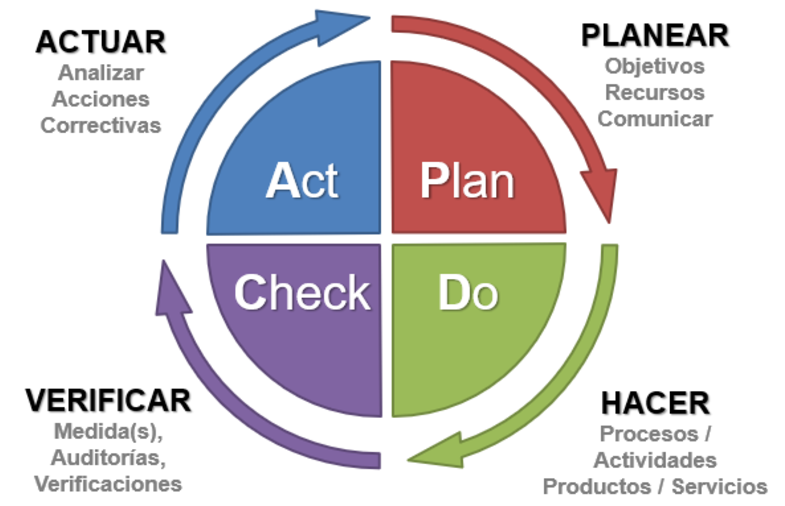
\includegraphics[scale=.4]{ciclo_deming.png}
    \caption{Ciclo Deming}
\end{figure}

Fases del ciclo de Deming:

\begin{enumerate}
    \item Planificar (Plan): Identificar un problema u oportunidad de mejora. Analizar la situación actual y definir objetivos. Diseñar un plan de acción con estrategias y recursos.

    \item Hacer (Do): Implementar el plan en una pequeña escala o fase de prueba. Ejecutar las acciones planificadas. Registrar datos y observaciones sobre el proceso

    \item Verificar (check): Evaluar los resultados obtenidos comparándolos con los objetivos. Analizar desviaciones y errores. Obtener aprendizajes para ajustar el proceso.

    \item Ajustar, actuar (act): Implementar las mejoras en toda la organización si el plan fue exitoso. Estandarizar los cambios y actualizar procedimientos. Si hay fallas, volver a la etapa de planificación y repetir el ciclo.
\end{enumerate}

\subsection{Las tres olas de Alvin Toffler}

Alvin Toffler, en su libro La Tercera Ola (1980), describe la evolución de la humanidad a través de tres grandes olas que representan cambios revolucionarios en la sociedad.

\begin{enumerate}
    \item Primera Ola: La Sociedad Agraria (8000 a.C. - Siglo XVIII): Surge con la Revolución Agrícola, cuando los humanos pasan de ser nómadas cazadores-recolectores a sociedades agrícolas. Se establecen comunidades rurales, basadas en la propiedad de la tierra y la producción de alimentos. La estructura social es feudal o tribal, con familias extensas y roles de género muy definidos. Se depende de la fuerza humana y animal para la producción. Impactos: Crecimiento de la población gracias a la estabilidad alimentaria. Sociedad rígida y con poco avance tecnológico.

    \item Segunda Ola: La Sociedad Industrial (Siglo XVIII - Mediados del Siglo XX): Nace con la Revolución Industrial, basada en la mecanización, el uso del carbón, el petróleo y la electricidad. La producción se traslada a fábricas y se impone el sistema de producción en masa (Fordismo). Se urbanizan las sociedades y crecen las ciudades. Aparece la educación estandarizada, el trabajo asalariado y la burocracia. Impacto: Avances tecnológicos masivos, crecimiento económico y mejoras en calidad de vida. Contaminación, explotación laboral y alienación del trabajador.

    \item Tercera Ola: La Sociedad de la Información (Desde mediados del Siglo XX - Presente): Surge con la Revolución Digital y la automatización, con el auge de la informática, las telecomunicaciones e Internet. Se pasa de una economía basada en la industria a una basada en el conocimiento y los servicios. La producción es flexible y personalizada, con trabajo remoto, globalización y descentralización. Se reduce la importancia del trabajo físico y crecen los sectores de tecnología, innovación y creatividad. Impacto: Acceso inmediato a la información, mayor innovación y conectividad global. Desigualdad digital, pérdida de empleos tradicionales por automatización y sobrecarga de información.

\end{enumerate}

\subsection{Evolución de la Industria}

\begin{figure} [ht!]
    \centering
    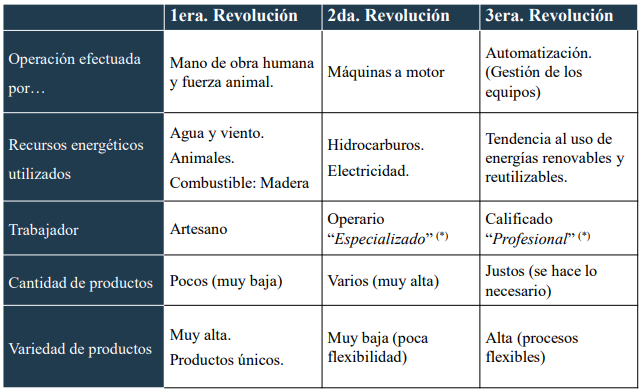
\includegraphics[scale=1]{evolucion_industrial.png}
    \caption{Cuadro comparativo}
\end{figure}

\begin{figure} [ht!]
    \centering
    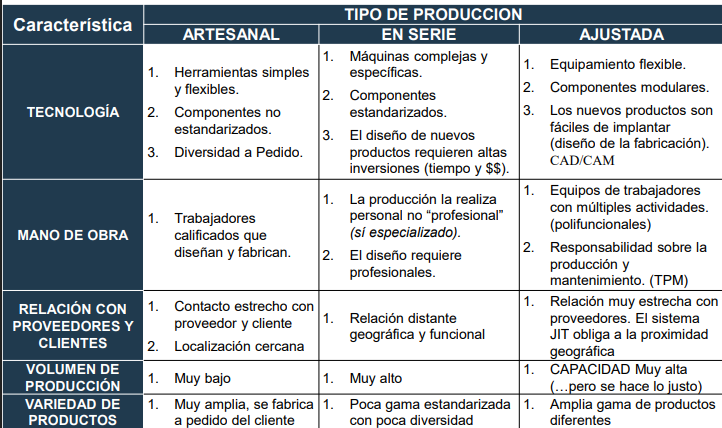
\includegraphics[scale=.85]{produccion.png}
    \caption{Tipos de producción}
\end{figure}

\begin{figure} [ht!]
    \centering
    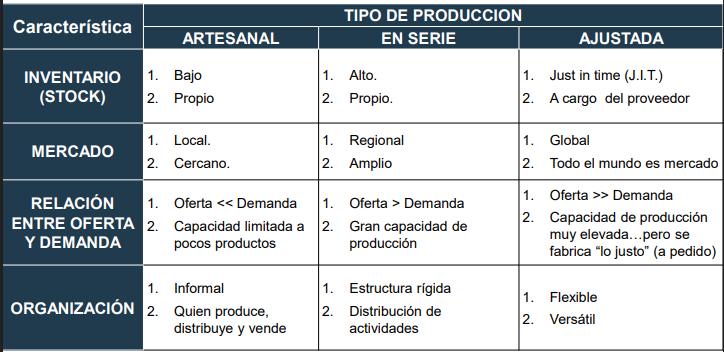
\includegraphics[scale=.85]{prod2.png}
    \caption{Tipos de prodcción}
\end{figure}

\newpage

\subsection{Industria 4.0}

La Industria 4.0 representa la evolución de la manufactura y los negocios hacia un entorno inteligente, interconectado y automatizado. Se basa en el uso avanzado de tecnologías digitales para optimizar la producción, mejorar la eficiencia y generar crecimiento mediante la integración de datos y sistemas ciberfísicos.

\textbf{Características clave de la Industria 4.0:}

\begin{itemize}
    \item Internet de las Cosas (IoT) e Internet Industrial de las Cosas (IIoT): Dispositivos y sensores conectados que permiten la comunicación en tiempo real entre máquinas y sistemas.
    \item Sistemas ciberfísicos (CPS): Integración de mecanismos físicos con algoritmos computacionales, permitiendo monitoreo y control en entornos digitales.
    \item Fabricación inteligente: Uso de manufactura digital, automatización avanzada y adaptabilidad para optimizar procesos y personalizar productos.
    \item Computación en la nube: Almacenamiento y procesamiento de grandes volúmenes de datos con acceso remoto y escalabilidad.
    \item Inteligencia Artificial (IA): Algoritmos capaces de analizar datos, predecir tendencias y optimizar operaciones industriales.
\end{itemize}

\textbf{Diferencia con la Tercera Revolución Industrial:}
\begin{itemize}
    \item Tercera Revolución Industrial: Digitalización de procesos, introducción de la automatización y el uso de computadoras en la manufactura.
    \item Cuarta Revolución Industrial: Potencia el impacto de la digitalización con inteligencia autónoma, interconectividad total y análisis de datos masivos para mejorar la toma de decisiones.
\end{itemize}
La Industria 4.0 no solo automatiza procesos, sino que permite que las máquinas se comuniquen entre sí, aprendan y optimicen la producción en tiempo real. 

\newpage

\section{Capitulo 2: Organización de la industria}

\subsection{Precursores}

\begin{enumerate}
    \item \textbf{Frederick W. Taylor}
    
        Frederick Winslow Taylor fue un ingeniero mecánico estadounidense considerado el padre de la Administración Científica. Su trabajo se centró en mejorar la eficiencia y productividad dentro de la industria, aplicando principios científicos al trabajo manual con el objetivo de eliminar desperdicios de tiempo y movimientos innecesarios. Taylor creía firmemente que, mediante la observación y la medición de cada tarea, era posible encontrar la mejor forma de realizarla, optimizando así los procesos productivos.

        En su teoría de la Organización Racional del Trabajo (ORT), Taylor estableció que el estudio del trabajo debía dividirse en dos fases principales. Primero, el análisis de métodos y tiempos, donde observaba detenidamente las tareas realizadas por los obreros, midiendo cada uno de sus movimientos para identificar maneras más eficientes de ejecutarlos. Luego, definió los principios fundamentales de la ORT, los cuales incluían la especialización del trabajador, la implementación de incentivos salariales basados en la productividad y el uso de análisis detallados para dividir las tareas en pasos estructurados.
        
        Uno de los conceptos clave en su teoría fue el del "Homo Economicus". Taylor sostenía que los trabajadores eran seres racionales motivados principalmente por incentivos económicos. Desde su perspectiva, un empleado que recibiera una recompensa monetaria directamente proporcional a su esfuerzo se desempeñaría de manera más eficiente. Por este motivo, implementó sistemas de pago basados en el rendimiento, donde los trabajadores más productivos obtenían mejores compensaciones económicas.
        
        El impacto de sus ideas fue significativo, ya que permitió aumentar la productividad y reducir costos en la industria, influyendo directamente en la evolución de la producción en masa y en la automatización de procesos. Gracias a su enfoque, muchas fábricas lograron mejorar sus métodos de trabajo, estableciendo procesos más ordenados y eficientes. Sin embargo, su sistema no estuvo exento de críticas. Muchos consideraban que Taylor deshumanizaba al trabajador, tratándolo como una máquina en lugar de una persona. La excesiva especialización de tareas, además, provocó monotonía y desgaste físico en los empleados, lo que llevó a cuestionamientos sobre el impacto psicológico de su modelo.
        
        A pesar de estas críticas, la Administración Científica de Taylor sentó las bases de la gestión moderna, influyendo en métodos actuales como la producción en cadena y el control de calidad. Su legado sigue vigente en la optimización de procesos industriales, demostrando que la eficiencia en el trabajo no es solo una cuestión de esfuerzo, sino también de organización y análisis científico.

    \item \textbf{Henri Fayol}
    
        Henri Fayol fue un ingeniero y teórico de la administración que desarrolló un enfoque integral sobre la gestión empresarial, centrándose en la estructura y el funcionamiento de las organizaciones. A diferencia de Frederick Taylor, quien analizaba el trabajo desde la perspectiva de la eficiencia operativa, Fayol se enfocó en el proceso administrativo y en cómo las funciones gerenciales podían mejorar la organización en su conjunto.

        Para Fayol, la administración era un acto compuesto por cinco funciones fundamentales: planificación, organización, dirección, coordinación y control. La planificación consistía en definir objetivos y establecer estrategias para alcanzarlos. La organización se refería a la asignación de recursos y la estructuración de las actividades. La dirección implicaba liderar y motivar a los empleados para ejecutar las tareas de manera efectiva. La coordinación buscaba armonizar todas las actividades de la empresa para que funcionaran en conjunto, y el control permitía evaluar si las acciones emprendidas estaban alineadas con los objetivos establecidos.
        
        Además, Fayol formuló 14 principios de administración, que sirvieron como guía para una gestión eficiente. Entre los más relevantes se encontraba la unidad de mando, que establecía que cada empleado debía recibir órdenes de un solo superior para evitar confusiones y conflictos. También destacó la importancia de la disciplina dentro de la organización, promoviendo reglas claras y el respeto a la autoridad. Otros principios clave incluían la división del trabajo, para mejorar la especialización y productividad, y la equidad, que señalaba la necesidad de un trato justo hacia los empleados.
        
        El enfoque de Fayol fue revolucionario porque proporcionó un marco estructurado para la gestión empresarial, aplicable no solo en la industria sino también en otras áreas organizacionales. Su visión de la administración como un conjunto de funciones universales permitió que sus principios fueran adoptados en diversas empresas y sectores.
        
        Aunque sus ideas fueron ampliamente aceptadas, también recibieron críticas. Algunos expertos consideraban que sus principios eran demasiado generales y no tenían en cuenta las dinámicas cambiantes de las organizaciones modernas. No obstante, su trabajo sentó las bases para la administración como disciplina formal y sigue siendo una referencia fundamental en la teoría de la gestión.

    \item \textbf{Henri Ford}

        Henry Ford fue un empresario e ingeniero estadounidense que revolucionó la industria automotriz con su modelo de producción basado en la eficiencia, la mecanización y la producción en masa. Su enfoque, conocido como fordismo, transformó la fabricación de automóviles y marcó un antes y un después en la organización del trabajo industrial.

        El fordismo se basó en la producción en serie, lo que permitió reducir costos y tiempos de fabricación. Ford implementó la línea de ensamblaje en sus fábricas, donde cada trabajador se especializaba en una tarea específica dentro del proceso de fabricación. Esto no solo aumentó la productividad, sino que también redujo la necesidad de capacitación extensa, ya que los empleados realizaban actividades repetitivas y altamente mecanizadas.
        
        Otro aspecto fundamental del fordismo fue la estandarización de los productos. Ford diseñó componentes intercambiables que facilitaban el ensamblaje y la reparación de los automóviles. Gracias a esta estrategia, logró producir vehículos a gran escala y venderlos a precios accesibles, democratizando el acceso al automóvil con su icónico Modelo T.
        
        Además, Ford implementó una integración vertical y horizontal en su empresa. Controlaba toda la cadena productiva, desde la extracción de materias primas hasta el ensamblaje final del producto, lo que le permitía optimizar costos y garantizar la calidad de los insumos. También diversificó sus operaciones al expandirse a otros sectores relacionados con la industria automotriz.
        
        El impacto del fordismo no se limitó solo a la producción, sino también a la organización del trabajo y la estructura social. Introdujo mejoras en las condiciones laborales, como la jornada de ocho horas y el pago de cinco dólares diarios, un salario superior al promedio de la época. Esta política no solo incentivó a los trabajadores, sino que también promovió el consumo, ya que muchos empleados podían permitirse comprar los automóviles que fabricaban.
        
        Otro cambio significativo fue la incorporación de mujeres en las fábricas, lo que amplió la participación de la mano de obra femenina en la industria. Sin embargo, el sistema fordista también recibió críticas. La repetitividad de las tareas generaba un trabajo monótono y agotador, y la rigidez del modelo dificultaba la adaptación a nuevas demandas del mercado.
        
        A pesar de sus limitaciones, el fordismo dejó un legado duradero en la producción industrial. Su enfoque en la eficiencia y la estandarización sentó las bases para la fabricación moderna y sigue siendo una referencia en la gestión de la producción a gran escala.

\end{enumerate}

\subsubsection{La producción ajustada (Lean Manufacturing)}

Es un modelo de gestión desarrollado en Japón, principalmente por Taiichi Ohno en Toyota, con el objetivo de optimizar los procesos de manufactura. Su enfoque se basa en la eliminación de desperdicios y la maximización del valor entregado al cliente final(cada proceso dentro de la producción debe centrarse en generar un beneficio real para el cliente, eliminando cualquier actividad que no aporte valor.).

Uno de sus principios fundamentales es la búsqueda de calidad perfecta desde la primera vez, lo que implica la detección y corrección de errores en su origen para evitar defectos en los productos. Además, se prioriza la minimización del despilfarro, eliminando todas aquellas actividades que no generan valor y optimizando el uso de recursos como capital, personal y espacio.

La mejora continua es otro pilar clave de este sistema, ya que busca reducir costos, mejorar la calidad y aumentar la productividad a través de la innovación constante y el intercambio de información dentro de la organización. A esto se suma la implementación de procesos “pull”, en los cuales la producción se ajusta a la demanda real del cliente, evitando la acumulación innecesaria de inventario.

Otro aspecto esencial del Lean Manufacturing es la flexibilidad en la producción, lo que permite fabricar distintos tipos de productos sin que esto afecte la eficiencia, incluso cuando los volúmenes de producción son reducidos. Además, se promueve una relación a largo plazo con los proveedores, basada en la cooperación para compartir riesgos, costos e información.

Desde el punto de vista operativo, el modelo introduce la organización de células de manufactura, donde máquinas, equipos y recursos se agrupan en áreas específicas para optimizar la producción. Asimismo, se reorganiza el trabajo en equipos siguiendo la secuencia del proceso de producción, asegurando que todas las operaciones necesarias para completar un producto estén integradas de manera eficiente.

Gracias a estas prácticas, el Lean Manufacturing ha permitido a las empresas reducir costos, mejorar la calidad y aumentar la capacidad de respuesta a la demanda del mercado, consolidándose como un sistema de producción altamente eficiente y adaptable.


\subsection{Tipos de organizaciones}

\begin{enumerate}
    \item Según el fin perseguido:
        \begin{itemize}
            \item \textbf{Organización empresarial:} Su principal objetivo es la obtención de beneficios económicos. Aunque su propósito fundamental es la rentabilidad, muchas de estas organizaciones también incorporan iniciativas sociales y medioambientales dentro de sus operaciones para mejorar su sostenibilidad y reputación. Ejemplo: Apple, Toyota, Coca Cola.
            \item \textbf{Organización sin ánimo de lucro:} Su propósito no es generar ganancias económicas, sino contribuir a causas sociales, medioambientales o de impacto en la comunidad. Estas organizaciones suelen depender de donaciones, subvenciones y voluntariado para llevar a cabo sus actividades. Ejemplo: Médicos sin fronteras, Greenpeace, Cruz Roja.
            \item \textbf{Organización no gubernamental:} Son entidades independientes del gobierno que brindan servicios públicos esenciales, como educación, sanidad o seguridad. Su función es complementar o cubrir áreas donde el sector público no llega de manera eficiente. 
        \end{itemize}

    \item Según la forma jurídica:
        \begin{itemize}
            \item Empresa privada: De propiedad particular, busca generar ganancias. Ejemplo: Google, Tesla, Nike.
            \item Empresa pública: Controlada por el Estado, suele ofrecer servicios esenciales. Ejemplo: YPF, Correo Argentino, Renfe.
            \item Empresa mixta: Combina inversión pública y privada. Ejemplo: Aerolíneas Argentinas.
            \item Empresa unipersonal: Propiedad de una sola persona, con control total sobre su gestión y beneficios.
        \end{itemize}

    \item  Según su alcance y estrategia de expansión:
    \begin{itemize}
        \item Empresa internacional: Operan en varios países pero centralizan la toma de decisiones en el país de origen. Ejemplo: vinos Argentino exportados a Europa
        \item Empresa multinacional: Opera en varios paises, pero con cierto grado de automnomía en cada ubicación, o cada filial adapta su estrategia al mercado local. Ejemplo: McDonald's
        \item Empresa global: Empresas con operaciones globales uniformes y centralizadas. Ejemplo: Una marca de ropa con productos idénticos en todo el mundo. Ejemplo: Apple (misma línea de productos en todo el mundo).
        \item Empresa transnacional: Buscan maximizar la eficiencia global permitiendo una mezcla de centralización y descentralización. Ejemplo: Una compañía tecnológica con centros de investigación en varios países para aprovechar talentos locales.
    \end{itemize}

    \begin{figure} [ht!]
        \centering
        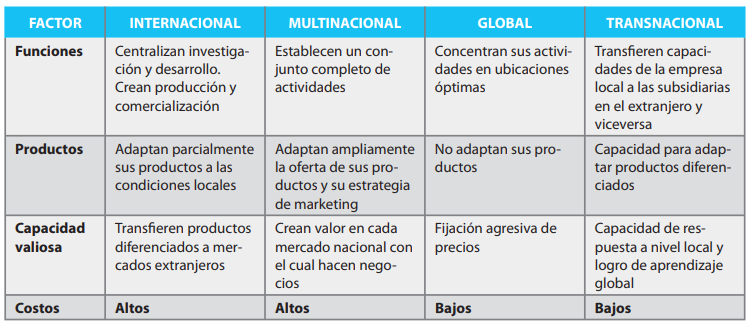
\includegraphics[scale=0.8]{cuadro alcance.png}
        \caption{Enter Caption}
        \label{fig:alcance}
    \end{figure}
\end{enumerate}


\subsection{Componentes de la organización empresarial}

Los componentes de la organización empresarial son fundamentales para estructurar y gestionar eficazmente una empresa, garantizando que sus objetivos se cumplan de manera eficiente.

\begin{enumerate}
    \item \textbf{Objetivo y eficiencia organizativa:} La organización facilita el logro de metas empresariales, mejora la comunicación interna y reduce la duplicación de esfuerzos al definir claramente las tareas de cada área.
    \item \textbf{Especialización laboral:} Asignar tareas según habilidades y conocimientos mejora la productividad y la calidad del trabajo.
    \item \textbf{Departamentos y compartimientos:} Dividir la empresa en áreas especializadas (finanzas, producción, recursos humanos, etc.) permite mayor eficiencia y colaboración.
    \item \textbf{Estructura orgánica y organigrama:} Define la jerarquía de la empresa, estableciendo roles y responsabilidades para un funcionamiento ordenado.
    \item \textbf{Normas y reglamentos:} Establecen lineamientos claros para la operación de la empresa, garantizando orden y coherencia en los procesos.
    \item \textbf{Infraestructura y recursos materiales:} Incluye máquinas, equipos, herramientas, talleres y oficinas, elementos esenciales para la producción y administración.
    \item \textbf{Recurso humano:} Las personas son el activo más importante de la empresa, aportando conocimientos, habilidades y creatividad al desarrollo organizacional.
\end{enumerate}


\subsection{Estructura Orgánica y Organigramas}

La estructura orgánica de una empresa es la forma en que se organizan y distribuyen las funciones, responsabilidades y jerarquías dentro de la organización. Define cómo se coordinan los recursos humanos y materiales para alcanzar los objetivos empresariales de manera eficiente.

\textbf{Características de una estructura orgánica:}

\begin{itemize}
    \item Jerarquía: Establece los niveles de autoridad y responsabilidad.
    \item Departamentalización: Agrupa actividades similares en áreas específicas (dpto finanzas, producción, ventas, etc.).
    \item Canales de comunicación: Define cómo fluye la información entre los distintos niveles y departamentos.
    \item Flexibilidad o rigidez: Puede ser más rígida (estructuras tradicionales) o flexible (organizaciones más innovadoras y dinámicas).
\end{itemize}

Las características comunes de un organigrama son las siguientes:

\begin{itemize}
    \item Departamentos y Responsables: Cada departamento se señaliza con su responsable a cargo.
    \item Conexiones entre Departamentos: Mediante flechas, se muestra cómo se relacionan las diferentes áreas entre sí.
    \item Refleja el Modo de Trabajar: Evidencia la forma en que la organización opera y se organiza internamente.
\end{itemize}

A continuación, se describen distintos tipos de organizaciones.

\textbf{Organización funcional:}

La organización funcional es una de las estructuras más utilizadas por las empresas debido a su claridad y eficiencia. Se desarrolla de forma jerárquica y vertical, organizando la empresa en departamentos según funciones específicas, como ventas, producción, finanzas o recursos humanos. Los líderes de la organización se ubican en la parte superior del organigrama, mientras que los empleados con menor autoridad ocupan los niveles inferiores.

Este modelo permite que cada área se especialice en su tarea, aumentando la eficiencia y asegurando que todas las partes de la empresa trabajen bajo una misma visión. Sin embargo, también puede generar poca comunicación entre departamentos y rigidez en la toma de decisiones. Es ideal para empresas que buscan una gestión centralizada y un crecimiento estructurado.

\begin{figure} [ht!]
    \centering
    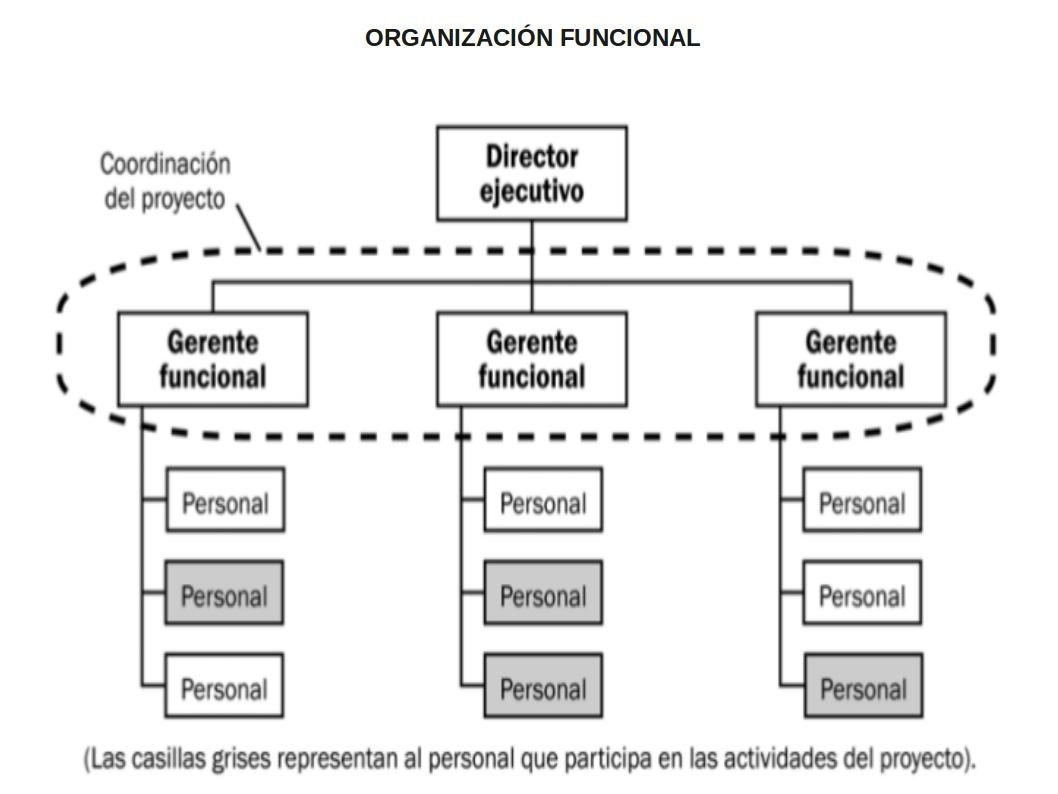
\includegraphics[scale=0.5]{org_funcional.jpg}
    \caption{Organización funcional}
\end{figure}

\textbf{Organización por producto:}

La organización por producto estructura la empresa en función de los diferentes bienes o servicios que ofrece. Cada línea de producto cuenta con su propio equipo de gestión, que incluye áreas como producción, ventas y marketing, permitiendo un enfoque especializado y una mayor adaptación a las necesidades del mercado.

Este modelo es común en empresas con una amplia gama de productos, como la industria automotriz o tecnológica, ya que facilita la innovación y mejora la competitividad. Sin embargo, puede generar duplicación de recursos y costos elevados debido a la independencia de cada unidad de negocio. Es ideal para empresas que buscan flexibilidad y autonomía en la gestión de sus productos.


\newpage


\section{Capitulo 3: Análisis del trabajo. Estudio de métodos.}


Concepto de organización: 

\begin{itemize}
    \item La organización es un sistema estructurado y dinámico compuesto por recursos humanos, materiales, tecnológicos y financieros, coordinados mediante un conjunto de normas, procedimientos y jerarquías con el fin de alcanzar objetivos específicos de manera eficiente y efectiva. Desde una perspectiva técnica, la organización se fundamenta en la división del trabajo, la asignación de funciones, la optimización de procesos y la gestión de la información, asegurando la interacción sinérgica entre sus elementos a través de principios de administración científica, teoría de sistemas y análisis de procesos.

    \item Objetivo principal de una empresa, obtener rédito económico
\end{itemize}



\subsection{Estudio del trabjo}

\subsubsection{Definición (según la OIT)}

El Estudio del Trabajo, según la Organización Internacional del Trabajo (OIT), es el conjunto de técnicas que se utilizan para analizar el trabajo humano en sus distintos contextos. Su propósito es investigar sistemáticamente todos los factores que afectan la eficiencia y economía de una determinada situación laboral, con el objetivo de proponer mejoras que optimicen el rendimiento, reduzcan costos y mejoren las condiciones de trabajo.

\begin{itemize}
    \item En todos sus contextos: 
    \item Sistemáticamente: ordenada, que ya ha sido probada. la finalidad es ser ordenado y metódico. Aprovechar la experiencia
    \item Lograr eficiencia y economiza: Logrando los objetivos propuestos empleando la menor cantidad de recursos posibles, más alla de los efectivamente disponibilidades. 
    Eficacia: lograr objetivo sin importara la cantidad de recursos consumidos
    Eficiencia: lograr objetivo sin importara la cantidad de recursos consumidos (5 ceros, eliminar todo aquello innecesario)
    \item A fin de efectuar mejoras: diseñando e implementando nuevas maneras de realizar las tares, que sean: más economicas, mas seguras, técnicamente posibles y convingentes, respetuosas con la ley y el medio ambiente.  
\end{itemize}

\subsubsection{Técnicas para el estudio de trabajo}

\begin{figure} [ht!]
    \centering
    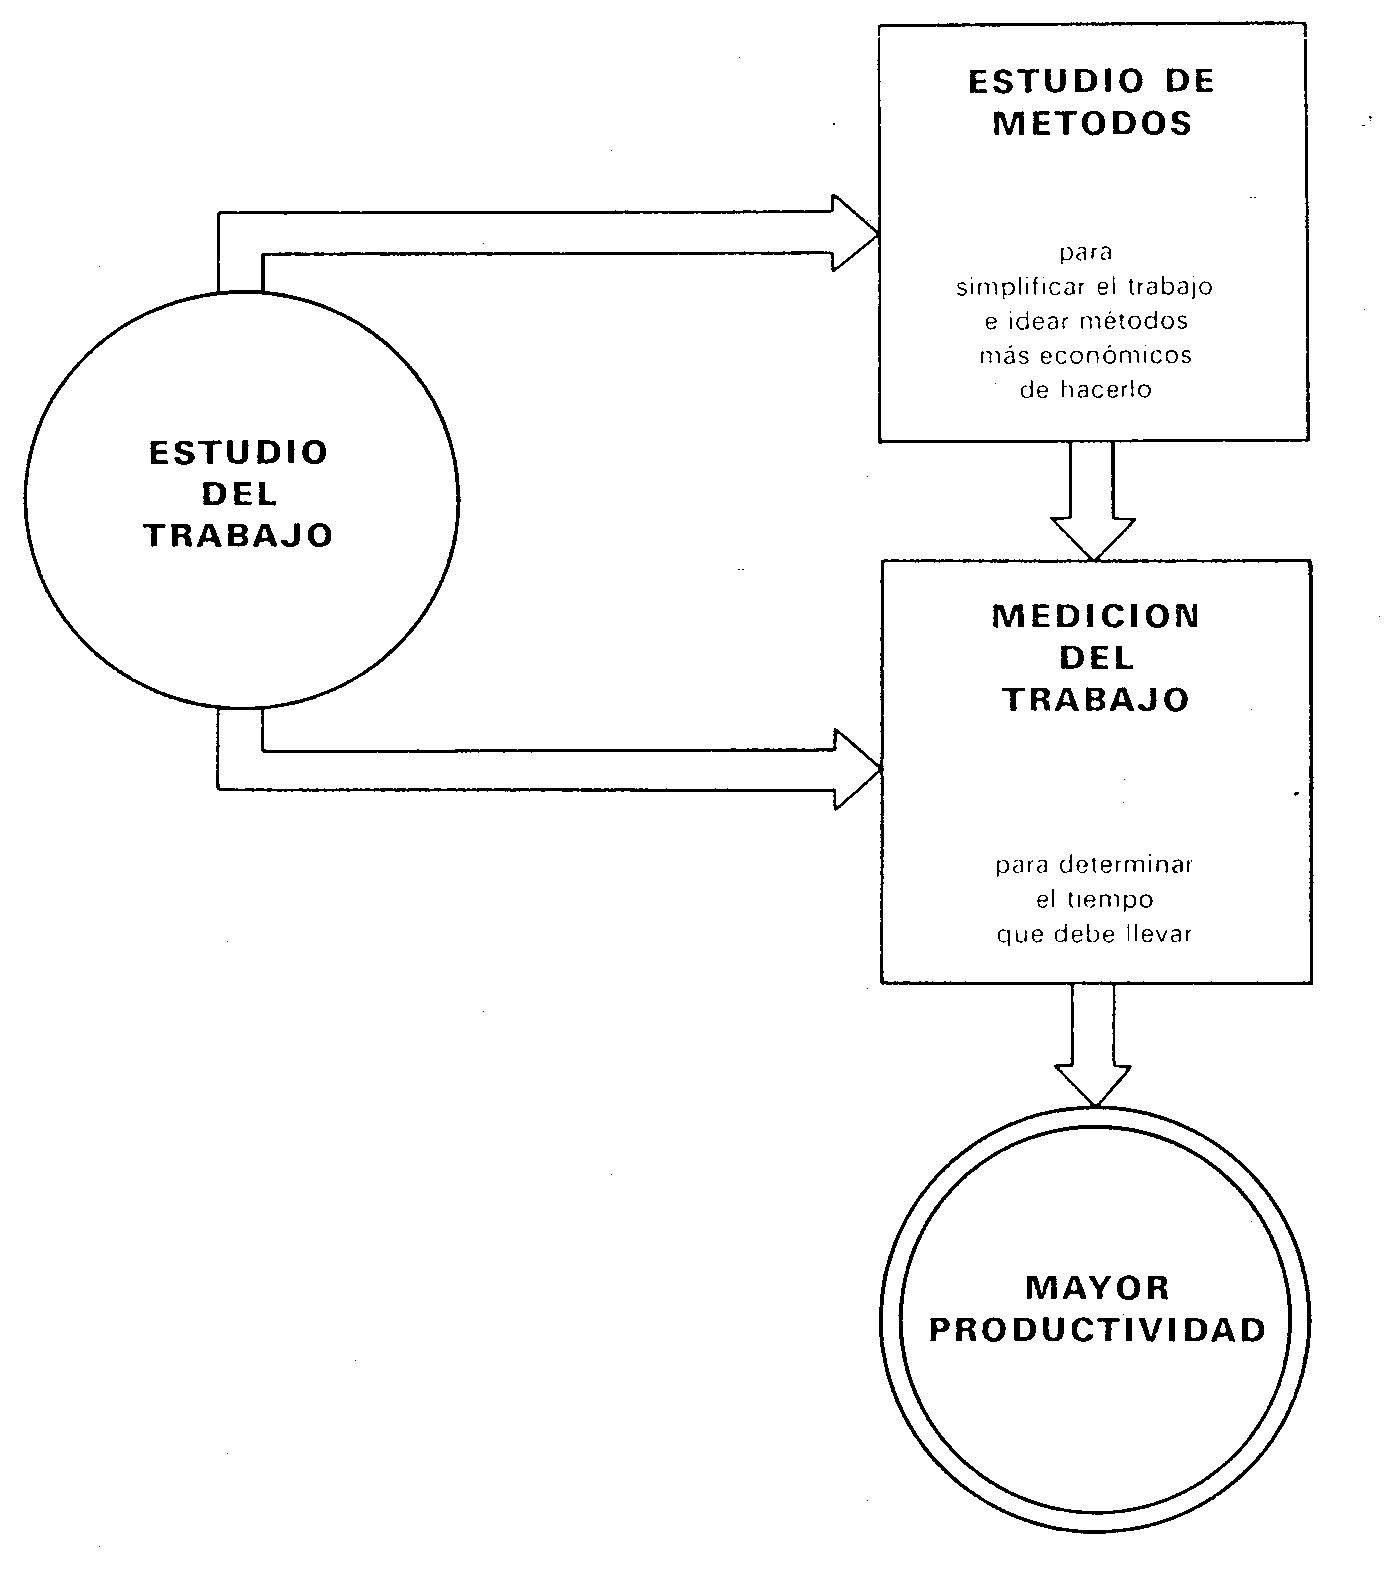
\includegraphics[width=0.5\linewidth]{tecnicas ET.png}
    \caption{Técnicas para el estudio de trabajo}
\end{figure}

El orden de los pasos en el Estudio del Trabajo es fundamental, ya que aplicar técnicas sin una secuencia lógica puede llevar a conclusiones erróneas o ineficientes.

\begin{itemize}
    \item Principio clave: No tiene sentido medir el tiempo de una tarea si primero no se ha optimizado su ejecución.
\end{itemize}

\subsubsection{Nivel de vida}

Grado de bienestar material del que dispone una persona, clase social o comunidad para sustentarse y disfrutar de la existencia.


El nivel de vida está determinado por la satisfacción de necesidades fundamentales, que garantizan el bienestar y la supervivencia. Estas incluyen:
\begin{itemize}
    \item Alimentación
    \item Vestido 
    \item Alojamiento
    \item Seguridad 
    \item Servicios esenciales
\end{itemize}

\subsubsection{Productividad}

La definición tradicional:

\begin{equation}
    PRODUCTIVIDAD = \dfrac{\text{CANTIDAD PRODUCIDA}}{\text{CANTIDAD DE RECURSOS UTILIZADOS}} = \dfrac{\text{OUTPUT}}{\text{INPUT}}
\end{equation}

En esta definición, los recursos utilizados pueden ser: tierra, materiales, instalaciones, maquinas y herramientas, servicio del hombre.

La nueva definición, de acuerdo a la norma ISO 9000 es: la productividad es la relación entre la cantidad de producción obtenida y los recursos utilizados para generarla. Es un indicador clave en cualquier actividad económica, ya que mide la eficiencia con la que se utilizan los insumos (materiales, energía, tiempo, capital, etc.).

La mano de obra no es un recurso de la empresa, sino es parte de la empresa.

Entonces, la definición moderna es:

\begin{equation}
    PRODUCTIVIDAD = \frac{\text{SATISFACCIÓN DEL CLIENTE}}{\text{RECURSOS EMPLEADOS INTELIGENTEMENTE}}
\end{equation}

Los recursos para esta nueva definición son: terrenos, edificios, maquinarias y equipos, materiales indirectos, horas maquinas, servicios auxiliares.

\textbf{Consideraciones:}
\begin{itemize}
    \item Las personas no son recursos de la empresa, son "la empresa".
    \item Las empresas no solo se deben encarar la productividad como un beneficio económico, sino también una inversión social y ambiental.
\end{itemize}

\subsubsection{Teorías sociales x e y}

Douglas McGregor formuló en 1960 las Teorías X e Y para explicar dos enfoques opuestos sobre la naturaleza del trabajador y la gestión dentro de una organización.


\paragraph{\textbf{Teoría X (Enfoque autoritario y de control):}}

La Teoría X parte de la premisa de que los trabajadores tienden a evitar el trabajo y requieren supervisión constante. Los supuestos del trabajador son:
\begin{itemize}
    \item Realiza sus tareas por obligación y bajo presión.
    \item Evita asumir responsabilidades y prefiere ser dirigido.
    \item Necesita dirección y supervisión continua.
    \item Su motivación proviene principalmente de recompensas externas o del temor a sanciones.
\end{itemize}

A menudo, esto proviene de la consecuencia de una gestión con:

\begin{itemize}
    \item Estilo de liderazgo autoritario y centralizado.
    \item Implementación de normas estrictas y sistemas de control rigurosos.
    \item Baja autonomía en la toma de decisiones.
    \item Clima laboral poco flexible, con riesgo de desmotivación y resistencia al cambio.
\end{itemize}

Este enfoque es aplicable en entornos donde las tareas son rutinarias y requieren un alto grado de disciplina y cumplimiento de procedimientos específicos. Sin embargo, puede generar un ambiente de trabajo poco estimulante y una disminución del compromiso del personal.


\paragraph{\textbf{Teoría Y (Enfoque participativo y motivador):}}

La Teoría Y plantea que los trabajadores pueden ser responsables, motivados y capaces de autogestión cuando se les proporciona un entorno adecuado. Los supuestos del trabajador son:


\begin{itemize}
    \item Es proactivo y asume responsabilidades de manera voluntaria.
    \item Disfruta de su trabajo cuando se le otorga libertad de acción.
    \item Su creatividad y capacidad de innovación se potencian en entornos flexibles.
    \item Encuentra satisfacción en el logro de sus tareas y en su desarrollo profesional.
    \item Es un activo estratégico dentro de la empresa.
\end{itemize}

A menudo, esto proviene de la consecuencia de una gestión con:


\begin{itemize}
    \item Estilo de liderazgo participativo, basado en la confianza.
    \item Mayor delegación de responsabilidades y fomento de la autonomía.
    \item Clima organizacional más dinámico y orientado al desarrollo del talento.
    \item Promoción de la creatividad, la innovación y el compromiso.
\end{itemize}

Este enfoque es más adecuado para organizaciones que buscan fomentar el desarrollo de sus empleados y promover la eficiencia a través de la motivación intrínseca.

\subsubsection{Teoria Z}

La Teoría Z, formulada por William Ouchi, propone un modelo de gestión empresarial basado en la integración de los principios de productividad y eficiencia con un enfoque en la estabilidad laboral y el desarrollo del capital humano. Su objetivo es maximizar el desempeño organizacional mediante la lealtad mutua entre la empresa y el trabajador, promoviendo una cultura corporativa sólida y orientada al largo plazo. Las caractreristicas principales, sonj:

\begin{itemize}
    \item Estabilidad laboral: Se privilegia el empleo fijo como estrategia para incrementar la productividad, reducir la rotación y minimizar los costos asociados a la capacitación y adaptación de nuevos trabajadores.
    \item Alto compromiso organizacional: Se busca que los empleados asuman un rol activo en la empresa, incrementando su sentido de pertenencia y su identificación con los objetivos corporativos.
    \item Trabajo en equipo: Se fomenta una estructura de trabajo colaborativa, priorizando la cooperación y la responsabilidad colectiva sobre la competencia individual.
    \item Reconocimiento basado en méritos: Los ascensos y el desarrollo profesional se fundamentan en la capacidad, el desempeño y la experiencia acumulada dentro de la organización.
    \item Participación en la toma de decisiones: Se impulsa la intervención del personal en los procesos estratégicos y operativos, promoviendo una gestión descentralizada y participativa.
\end{itemize}

La aplicación de la Teoría Z permite una mayor eficiencia operativa mediante la optimización de los recursos humanos y la consolidación de una cultura organizacional comprometida con la mejora continua. La combinación de estabilidad laboral, reconocimiento y participación activa favorece la reducción de conflictos internos y la optimización del rendimiento, generando una ventaja competitiva sostenible en el tiempo.

En simples palabras: el modelo apuesta por el empleo de "por vida", confianza total en los empleados, toma de decisiones en grupo, desarrollo lento pero estable, cultura fuerte y compartida en la empresa. Propone que si tratas bien a la gente, les das estabilidad, los haces parte de las decisiones y fomentas una cultura sólida, van a rendir más, comprometerse más y querer quedarse en la empresa. Es ideal para empresas que quieren retener talento, mejorar el compromiso interno y potenciar el trabajo en equipo, sobre todo en sectores donde el conocimiento interno y la experiencia son claves (sí, ingeniería incluida).

\subsubsection{Producción vs productividad}

Los conceptos de producción y productividad tienen diferencias fundamentales en su significado y aplicación dentro de la gestión industrial y empresarial.

\begin{itemize}
    \item \textbf{Producción:} cantidad total de bienes o servicios generados en un proceso productivo dentro de un período determinado. Es una medida absoluta, sin considerar la eficiencia con la que se emplean los recursos.

    \item \textbf{Productividad:} mide la eficiencia con la que se utilizan los recursos (insumos) para obtener un determinado nivel de producción.
\end{itemize}

La relación entre ambos conceptos,

\begin{itemize}
    \item Un aumento en la producción no implica necesariamente un aumento en la productividad.
    \item Si la producción se incrementa pero en igual proporción se incrementa el uso de recursos, la productividad permanece constante.
    \item La productividad solo mejora si se logra producir más con los mismos recursos o producir lo mismo con menos recursos.
\end{itemize}

\paragraph{\textit{Ejemplo práctico: Caso sin mejora en la productividad}}

Se fabrican 1.000 piezas utilizando 100 trabajadores.
Se aumenta la producción a 2.000 piezas, pero contratando 200 trabajadores.
La productividad no cambia, ya que la relación entre producción y recursos se mantiene.

Caso con mejora en la productividad:
Se mantienen los 100 trabajadores, pero se optimizan procesos y se fabrican 1.500 piezas en lugar de 1.000.
La productividad aumenta, porque con los mismos recursos se obtiene una mayor producción.


\subsection{\textit{A. ESTUDIO DE MÉTODOS}}

El Estudio de Métodos, según la Organización Internacional del Trabajo (OIT), es el \textit{registro} y \textit{examen crítico sistemático} de los \textit{métodos actuales y proyectados} para llevar a cabo un trabajo, con el objetivo de \textit{idear y aplicar} procedimientos más \textit{eficientes}, simplificar operaciones y \textit{reducir costos}.

El procedimiento básico para el estudio de métodos:

\begin{enumerate}
    \item \textit{\textbf{Seleccionar:}} Identificar la tarea, operación o proceso que requiere optimización. Se priorizan actividades con mayor impacto en costos, tiempo y seguridad.

    \item \textit{\textbf{Registrar:}} Documentar detalladamente el método actual utilizando herramientas como diagramas de flujo, listas de verificación o estudios de tiempos. Recoger datos objetivos sobre la secuencia de trabajo, movimientos y tiempos empleados.

    \item \textit{\textbf{Examinar:}} Analizar críticamente cada etapa del proceso. Cuestionar cada paso con preguntas clave: ¿Qué? ¿Por qué? ¿Dónde? ¿Cuándo? ¿Quién? ¿Cómo? Detectar actividades innecesarias, movimientos ineficientes y oportunidades de mejora. 

    \item \textit{\textbf{Idear:}} Diseñar nuevas alternativas para optimizar el proceso. Aplicar principios de simplificación del trabajo, ergonomía y reducción de desperdicios.

    \item \textit{\textbf{Definir:}} Seleccionar la mejor alternativa considerando su viabilidad técnica y económica. Desarrollar procedimientos estándar para su correcta ejecución.

    \item \textit{\textbf{Implementar:}} Poner en práctica el nuevo método en condiciones reales. Capacitar al personal y ajustar el proceso según los resultados obtenidos.

    \item \textit{\textbf{Mantener en uso:}} Asegurar la aplicación continua del método mejorado. Realizar seguimiento y mejora continua para evitar el retorno a prácticas ineficientes.
\end{enumerate}

\subsubsection{Objetivos del estudio de métodos:}

\begin{itemize}
    \item Mejorar los procesos y los procedimientos.
    \item Mejorar la disposición de la fabrica, taller y lugar de trabajo, así como los modelos de máquinas e instalaciones.
    \item Economizar esfuerzo humano y reducir la fatiga innecesaria
    \item Mejorar la utilización de los materiales, máquinas y mano de obra
    \item Crear mejores condiciones materiales de trabajo
\end{itemize}

\subsection{1°-SELECCIONAR}

El primer paso en el Estudio de Métodos es la selección de la tarea, operación o proceso que será objeto de análisis y optimización. Para ello, es fundamental considerar distintos criterios de evaluación, asegurando que el esfuerzo de mejora tenga un impacto significativo.

Los criterios de selección o 'consideraciones de índole':

\begin{itemize}
    \item Económicos: Siempre debemos preguntarnos si valdrá la pena arrancar el estudio de métodos para este trabajo/proceso!. Procesos con altos costos operativos (materias primas, energía, desperdicio). Operaciones que representen cuellos de botella en la producción. Áreas con bajo rendimiento o productividad, afectando la rentabilidad. Ejemplos: atascos, desplazamientos de materiales innecesarios, gran cantidad de mano de obra o manipulación repetida de materiales

    \item Técnicos y tecnológicos: Métodos que utilicen equipos obsoletos o ineficientes. Procesos con excesiva variabilidad en tiempos o calidad. Posibilidades de automatización o mecanización. También, debemos 'saber' si es posible 'acelerar' un proceso.

    \item Humanos: Actividades con altos niveles de fatiga, esfuerzo o riesgo ergonómico. Procesos con alto índice de errores o retrabajos, que podrían mejorarse mediante capacitación o rediseño. Métodos que generen insatisfacción laboral o falta de motivación.

    \item Legales/Normativas: Cumplimiento de normas de seguridad e higiene en el trabajo. Regulaciones sobre medio ambiente, calidad y condiciones laborales. Procesos con potenciales riesgos legales o incumplimientos normativos.
\end{itemize}

El hecho de seleccionar bajo un aspecto, no es excluyente. El seleccionamiento de uno de ellos repercute sobre los otros.

\subsection{2°-REGISTRAR}

 Por medio de la observación directa, todo lo que sea pertinente al método actual. Se emplean técnicas de registro según se el propósito o aspecto que se desee evidenciar: sucesión, tiempo o movimiento. 'El éxito del proceso depende del grado de exactitud con que se registran los hechos'. Es esencial que sean claras y concisas.

 Para evitar dificultades, se idearon técnicas e instrumentos de anotación.

 \vspace{.5cm} % Deja 1 cm de espacio

 \newenvironment{subgroup}
  {$\left\{\tabular{l}}
  {\endtabular\right.$}
  
Gráficos / diagramas
\begin{subgroup}
  indican SUCESION
  \begin{subgroup}
    Cursograma sinópitico del proceso \\
    Cursograma analítico del operario / maquina \\
    / material\\
    Diagrama bimanual
  \end{subgroup} \\[2em]
  con ESCALA DE TIEMPO
  \begin{subgroup}
    Diagrama de actividades múltiples \\
    Simograma 
  \end{subgroup} \\[2em]
  indican MOVIMINETO
  \begin{subgroup}
    Diagrama de recorrido o circuito \\
    Diagrama de hilos \\
    Ciclograma\\
    Cronociclograma\\
    Gráfico de trayectoria
  \end{subgroup}
\end{subgroup}

\subsubsection{Gráficos que indican SUCESIÓN}
\begin{itemize}
    \item \textbf{\textit{Cursograma sinóptico del proceso}}

        Es un gráfico utilizado para representar de manera esquemática la sucesión de actividades dentro de un proceso. De la simbología, \textbf{solo se utilizan las OPERACIONES Y PROCESO}.

        \textit{Características del cursograma sinóptico:}
        \begin{itemize}
            \item Representa las operaciones, inspecciones, transportes, demoras y almacenamientos mediante símbolos estandarizados.
            \item Permite identificar ineficiencias, cuellos de botella y actividades innecesarias.
            \item Se emplea como base para la mejora de métodos mediante la eliminación, combinación o reordenamiento de tareas.
        \end{itemize}

        La simbología usada en el cursograma sinóptico del proceso se muestra en la siguiente imagen.

        \begin{figure} [ht!]
            \centering
            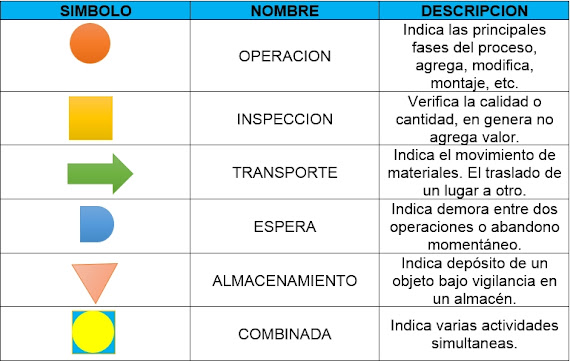
\includegraphics[scale=0.65]{simbologia.png}
            \caption{Enter Caption}
        \end{figure}
        

        De derecha a izquierda, al componer los elementos, siendo el primero el que se le ensamblan los elementos. (derecha)
        
        Este gráfico facilita una visión global y estructurada del proceso, ayudando a optimizar la secuencia de trabajo.

        Un ejemplo, lo podemos encontrar en el anexo, en la figura \ref{fig:csdp}
        
    \item \textbf{\textit{Cursograma analítico del operario / del material / de la máquina o equipo}}
    
        Permite representar de manera gráfica y detallada la sucesión de actividades en un proceso productivo. Puede aplicarse a distintos elementos dentro de la producción:
        \begin{itemize}
            \item Del operario: Registra las actividades realizadas por un trabajador en un proceso determinado.
            \item Del material: Muestra el flujo del material a lo largo del proceso productivo.
            \item De la máquina o equipo: Representa el uso y funcionamiento de una máquina o equipo en la producción.
        \end{itemize}
        Se registra el desarrollo del trabajo en una hoja proforma, detallando cada operación, inspección, transporte, demora y almacenamiento. Se utiliza la simbología indicada anteriormente. En el anexo, justamente en la figura \ref{fig:proforma} podemos identificar un ejemplo.
    \item \textbf{\textit{Diagrama bimanual}}
    
        Es una representación gráfica que registra los micromovimientos de ambas manos de manera independiente durante la ejecución de una tarea. Su propósito es optimizar la disposición del puesto de trabajo, eliminando movimientos innecesarios y mejorando la eficiencia operativa. Permite identificar y racionalizar la sucesión de acciones, facilitando la sincronización y reducción de tiempos improductivos.

        En la figura \ref{fig:bimanual} se adjunta un ejemplo. \label{ref:volver3}
    
\end{itemize}

\subsubsection{Gráficos que indican TIEMPO}
\begin{itemize}
    \item \textbf{\textit{Diagrama de actividades múltiples.}}
    
        Conocido como Diagrama Hombre-Máquina, es una herramienta gráfica utilizada para coordinar la interacción entre operarios y equipos en procesos productivos o de mantenimiento. Permite visualizar la secuencia de actividades de cada elemento involucrado, identificando tiempos muertos y optimizando la asignación de recursos. Es especialmente útil en producción en serie y en situaciones donde es crítico minimizar el tiempo de inactividad de maquinaria costosa. Además, facilita la determinación del número óptimo de máquinas que un operario o grupo de operarios puede atender eficientemente.
    \item \textbf{\textit{Simograma}}

    Consiste en un registro cinematográfico donde se mide el tiempo empleado en cada micromovimiento, asignándolo a un elemento definido como therblig (según Frank y Lilian Gilbreth).

    El procedimiento se realiza filmando a velocidad constante y contando los cuadros transcurridos entre el inicio y la finalización de cada therblig.
    
    Hoy en día, con el reemplazo de las películas en celuloide por sistemas digitales, este proceso se ha vuelto aún más simple y preciso.
\end{itemize}

\subsubsection{Gráficos que indican MOVIMIENTO}
\begin{itemize}
    \item \textbf{\textit{Diagrama de recorrido o circuito}}
    
    Representa el desplazamiento de operarios, materiales o equipos dentro de un área de trabajo. Se elabora sobre un plano del lugar, trazando las rutas seguidas y permitiendo detectar recorridos innecesarios o superposiciones que puedan optimizarse. El plano no necesariamente debe estar a escala. Suele ir acompañado del cursograma del objeto.
    
    \item \textbf{\textit{Diagrama de hilos}}

    Se utiliza para analizar el movimiento de un operario o material dentro de un proceso. Consiste en fijar un hilo sobre un plano a escala, siguiendo la trayectoria real del desplazamiento. Es útil para evaluar la eficiencia del recorrido y reducir trayectorias excesivas.
    
    \item \textbf{\textit{Ciclograma}}

    Registra los movimientos de una parte del cuerpo o de una herramienta mediante una fuente de luz intermitente (estroboscopio), generando una secuencia de imágenes superpuestas que permite analizar trayectorias y mejorar la ergonomía del trabajo.

    \begin{figure} [ht!]
        \centering
        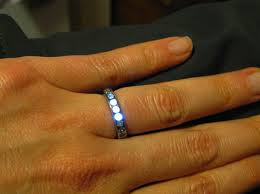
\includegraphics[width=0.5\linewidth]{anillo.png}
        \caption{Enter Caption}
        \label{fig:anillo}
    \end{figure}
    
    \item \textbf{\textit{Cronociclograma}}

    Variante del ciclograma que incorpora marcas de tiempo en los trazos luminosos, lo que permite medir la velocidad y frecuencia de cada movimiento. Se utiliza para identificar movimientos innecesarios y mejorar la eficiencia en tareas repetitivas.
    
    \item \textbf{\textit{Gráfico de trayectoria}}

    Representa visualmente el desplazamiento de un objeto, operario o herramienta en un espacio determinado. Se emplea para estudiar patrones de movimiento, mejorar la disposición del área de trabajo y optimizar recorridos en procesos industriales.
\end{itemize}

\subsection{3°-EXAMINAR}

Analizar con espíritu crítico la información recopilada en la fase anterior, de forma estructurada y utilizando las técnicas más adecuadas según el caso. En esta etapa se aplica la primera fase de la técnica del interrogatorio, cuestionando cada aspecto del proceso para identificar posibles mejoras, eliminaciones de desperdicios y oportunidades de optimización.

Se analiza detalladamente la información obtenida en la fase de observación y registro, con el objetivo de detectar ineficiencias, redundancias o posibles mejoras en el método actual.

En esta fase, se formulan preguntas clave para evaluar la necesidad y eficiencia de cada actividad registrada. Se analizan cinco aspectos fundamentales:

\begin{itemize}
    \item Propósito → ¿Para qué se realiza esta actividad?, Que se hace en ralidad?
    \item Lugar → ¿Dónde se lleva a cabo y es el sitio más adecuado?
    \item Sucesión → ¿El orden en que se realiza es el óptimo?
    \item Responsable / persona  → ¿Quién la ejecuta y es la persona indicada?
    \item Medios → ¿Con qué recursos se lleva a cabo y pueden mejorarse?
\end{itemize}

El objetivo de este análisis es detectar mejoras potenciales, aplicando uno o más de los siguientes enfoques:

\begin{itemize}
    \item Eliminar actividades innecesarias
    \item Reordenar la secuencia de tareas
    \item Combinar pasos para optimizar el flujo de trabajo
    \item Simplificar procesos para reducir tiempos y esfuerzos
\end{itemize}

Las preguntas de la 1ª etapa de la Técnica del Interrogatorio deben formularse en modo imperativo para realizar un revelamiento estructurado y objetivo del proceso actual. De este modo, se obtiene una visión crítica y sistemática de cada actividad.

\begin{itemize}
    \item ¿Qué se hace? → ¿Es esencial esta actividad? ¿Puede eliminarse o reducirse?
    \item ¿Dónde se hace? → ¿El lugar es el más adecuado o se puede optimizar su ubicación?
    \item ¿Cuándo se hace? → ¿El momento en que se realiza es el más eficiente? ¿Puede reorganizarse?
    \item ¿Quién lo hace? → ¿Es la persona idónea para la tarea o puede delegarse mejor?
    \item ¿Cómo se hace? → ¿Es el método más eficiente o se puede simplificar?
    \item ¿Con qué se hace? → ¿Los medios utilizados son los mejores o pueden mejorarse?
\end{itemize}

\subsection{4°-IDEAR}

En esta etapa se diseña el método más práctico, económico y eficaz, considerando todas las contingencias posibles. Se busca optimizar el proceso con un enfoque sistemático y estructurado.

\textbf{\textit{2ª Etapa de la Técnica del Interrogatorio (Preguntas de Fondo)}}

Las preguntas se formulan en modo condicional para evaluar las posibles mejoras que se pueden implementar.
\begin{itemize}
    \item Propósito: ¿Qué otra cosa se podría o debería hacer?
    \item Lugar: ¿En qué otro lugar se podría o debería hacer?
    \item Sucesión: ¿En qué otro momento se podría o debería hacer?
    \item Persona: ¿Quién otro lo podría o debería hacer?
    \item Medios: ¿De qué otro modo se podría o debería hacer?
\end{itemize}

Este análisis permite definir un futuro mejorado del proceso, considerando alternativas más eficientes y viables.

\subsection{5°-DEFINIR}

En esta fase se establece y documenta el nuevo método optimizado, asegurando que \textit{pueda ser identificado, comprendido y aplicado en cualquier momento}. Los objetivos principales son:

\begin{itemize}
    \item Estandarizar el nuevo procedimiento para garantizar su correcta implementación.
    \item Comparar con el método anterior, verificando las mejoras obtenidas.
    \item Facilitar la capacitación del personal y la replicabilidad del proceso.
    \item Asegurar la calidad y eficiencia en la ejecución del trabajo.
\end{itemize}

Para mantener coherencia y trazabilidad, se recomienda utilizar las mismas técnicas de registro aplicadas en la etapa inicial. Esto permite una comparación directa entre el método antiguo y el nuevo, demostrando las mejoras en términos de tiempos, costos y eficiencia.

Existen tres documentos porque son fundamentales para formalizar, estandarizar y asegurar la correcta implementación del nuevo método. Estos documentos no son opcionales, sino que sirven para que el nuevo proceso se aplique correctamente en la práctica y para que cualquier persona involucrada en la operación pueda seguirlo de manera precisa. La diferencia clave es:
\begin{itemize}
    \item Los gráficos y registros previos (como diagramas de flujo, cursogramas, etc.) sirven para analizar el proceso y compararlo con el anterior.
    \item La hoja de ruta, ficha de operación e instrucciones de inspección son documentos de uso operativo que formalizan el nuevo método y guían a los trabajadores.
\end{itemize}

Detallando los gráficos:

\begin{itemize}
    \item \textbf{\textit{Hoja de ruta:}} Documento que detalla las actividades a realizar en cada puesto de trabajo, siguiendo la secuencia establecida del proceso productivo. Su numeración suele realizarse en intervalos de 10 (10, 20, 30...), permitiendo la inclusión de futuras operaciones sin alterar el orden general.

    \item \textbf{\textit{Ficha de operación:}} Documento técnico que describe en detalle cada tarea dentro de un proceso productivo, asegurando uniformidad en la ejecución. Incluye: descripción de la operación, herramientas y materiales requeridos, parámetros de control, normas de seguridad, secuencia de trabajo.

    \item \textbf{\textit{Instrucciones de inspección:}} Documento que especifica los criterios y métodos para verificar la calidad de un producto o proceso. Define: características a inspeccionar (dimensiones, acabados, ensamblaje, etc.), instrumentos de medición y tolerancias permitidas, frecuencia y tipo de inspección (visual, dimensional, funcional, etc.), acciones correctivas en caso de no conformidad. Garantiza que los productos cumplan con los estándares establecidos y permite detectar desviaciones en etapas tempranas.
\end{itemize}


\subsection{6°-IMPLEMENTAR}

Esta etapa consiste en establecer el nuevo método como práctica estándar en la operación. Para lograrlo, se deben llevar a cabo las siguientes acciones:

\begin{enumerate}
    \item \textbf{\textit{Capacitación del personal}}
    \begin{itemize}
        \item Asegurar que los operarios comprendan y dominen el nuevo procedimiento.
        \item Utilizar documentos de apoyo como fichas de operación e instrucciones de inspección.
        \item Realizar entrenamientos prácticos para minimizar errores en la implementación.
    \end{itemize}
    \item \textbf{\textit{Eliminación del método anterior}}
    \begin{itemize}
        \item Retirar documentación, herramientas o dispositivos asociados al procedimiento obsoleto.
        \item Evitar la coexistencia de ambos métodos para prevenir confusiones y desviaciones.
    \end{itemize}
\end{enumerate}

El éxito de esta fase depende de la correcta gestión del cambio y de un seguimiento adecuado para verificar la adopción del nuevo sistema.

\subsection{7°-MANTENER EN USO}

Una vez implantado el nuevo método, es fundamental asegurar su permanencia como práctica habitual. Esto se logra a través de un control riguroso y una supervisión continua para evitar que los operarios vuelvan a aplicar el método anterior.

\begin{enumerate}
    \item \textbf{Supervisión y auditoría periódica:}
    \begin{itemize}
        \item Verificar que las tareas se ejecuten de acuerdo con los procedimientos establecidos.
        \item Identificar posibles desviaciones o errores en la aplicación del método.
        \item Usar listas de verificación o inspecciones programadas para garantizar la correcta implementación.
    \end{itemize}
    
    \item \textbf{Refuerzo en la capacitación:}
    \begin{itemize}
        \item Realizar reuniones periódicas para reforzar la importancia del nuevo método.
        \item Atender dudas o dificultades que puedan surgir en la práctica.
        \item Ofrecer formación continua para evitar la pérdida de habilidades adquiridas.
    \end{itemize}
    
    \item \textbf{Corrección de desviaciones:}
    \begin{itemize}
        \item Si se detecta que los operarios tienden a volver al método anterior, analizar las causas.
        \item Implementar medidas correctivas, como ajustes en la capacitación o modificación de ciertos aspectos del método si resultan poco prácticos.
        \item Asegurar que las herramientas y documentación disponibles faciliten la correcta aplicación del método nuevo.
    \end{itemize}
    
    \item \textbf{Adaptabilidad y mejora continua:}
    \begin{itemize}
        \item Evaluar periódicamente el desempeño del método implementado.
        \item Considerar ajustes o mejoras si se identifican oportunidades de optimización.
        \item Fomentar la retroalimentación del personal para detectar problemas o sugerencias de mejora.
    \end{itemize}
\end{enumerate}

Dado que, por naturaleza, los trabajadores pueden tender a volver al método anterior por costumbre o comodidad, es esencial que los responsables del proceso mantengan un seguimiento constante y refuercen la aplicación del nuevo sistema hasta que se convierta en la norma establecida

\newpage

\section{ANEXO} 

\begin{figure} [ht!]
    \centering
    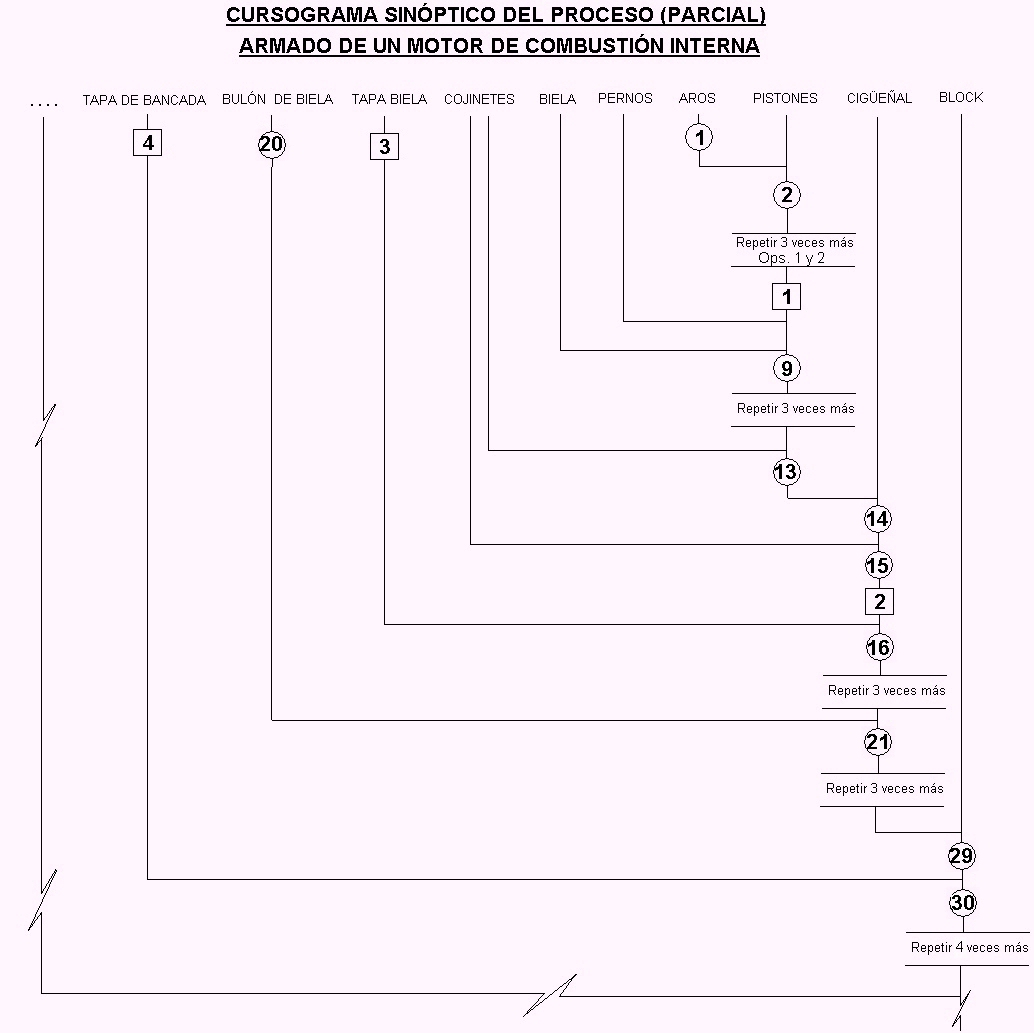
\includegraphics[scale=.9]{curso sinoptico del proceso.png}
    \caption{Cursograma sinóptico del proceso}
    \label{fig:csdp}
\end{figure}

\begin{figure} [ht!]
    \centering
    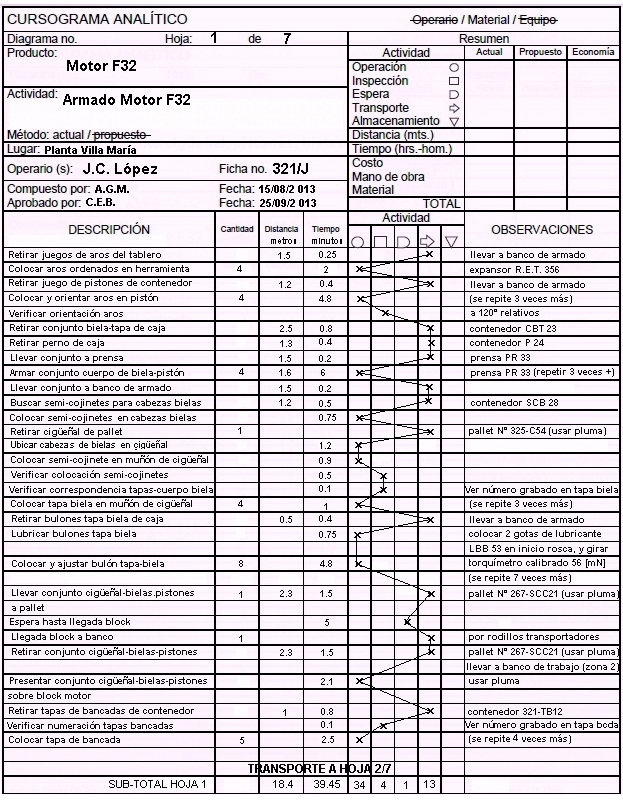
\includegraphics[scale=1.1]{proforma.png}
    \caption{Cursograma analítico}
    \label{fig:proforma}
\end{figure}

\begin{figure} [ht!]
    \centering
    \rotatebox{90}{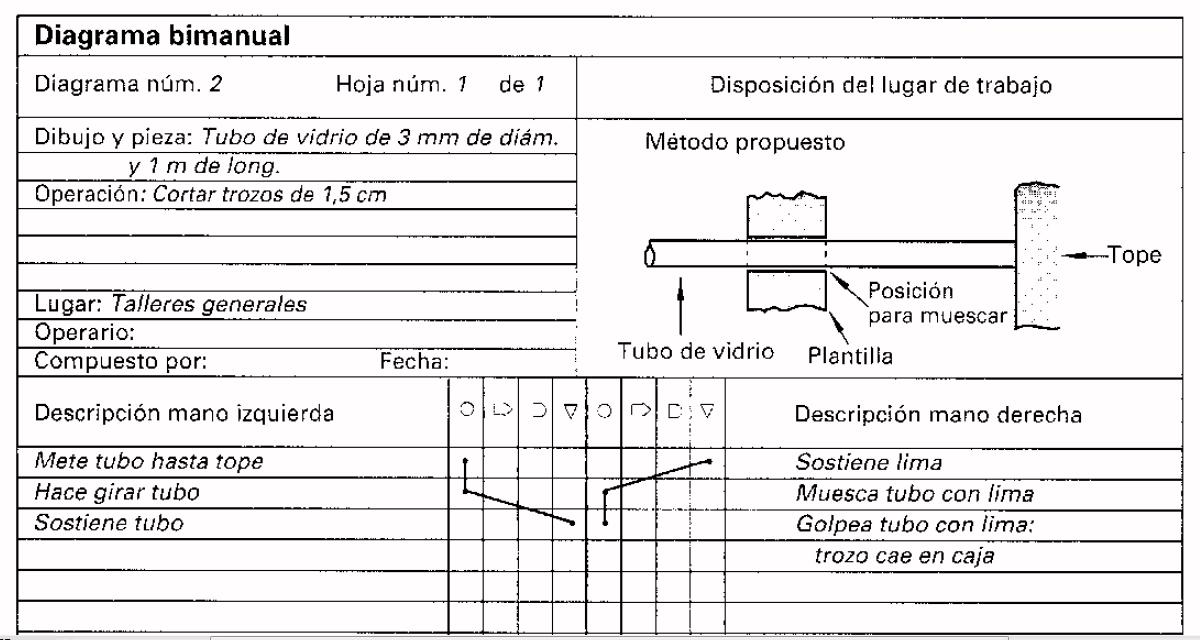
\includegraphics[scale=.85]{bimanual.png}}
    \caption{Diagrama bimanual - volver a \ref{ref:volver3}}
    \label{fig:bimanual}
\end{figure}

\begin{figure} [ht!]
    \centering
    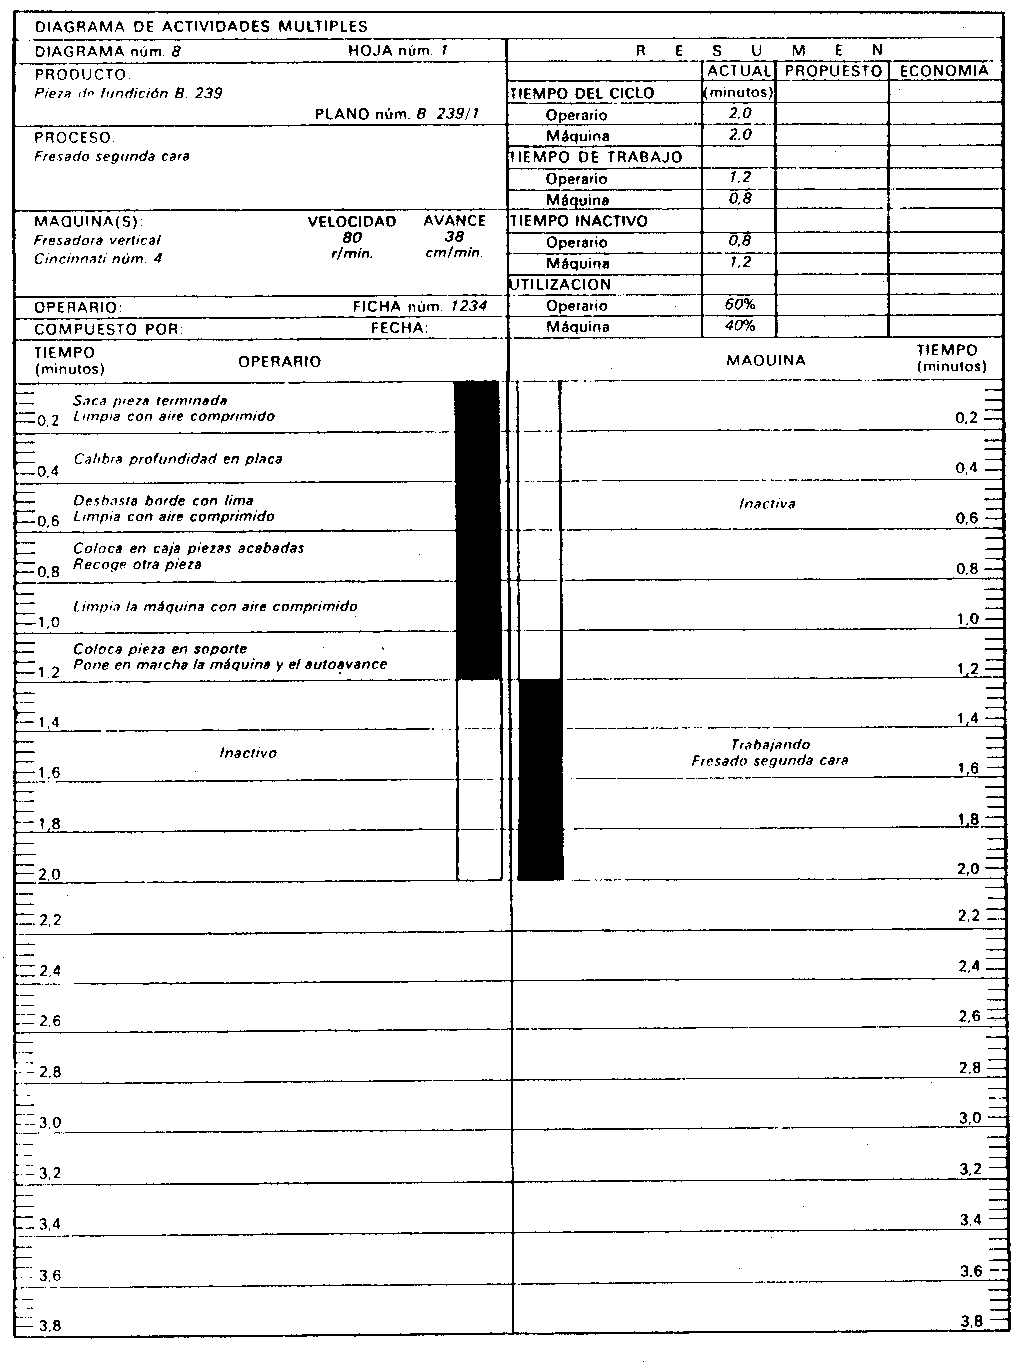
\includegraphics[scale=1.3]{actividades multiples.png}
    \caption{Diagrama de actividades múltiples 'actual'}
    \label{fig:act mult}
\end{figure}


\begin{figure} [ht!]
    \centering
    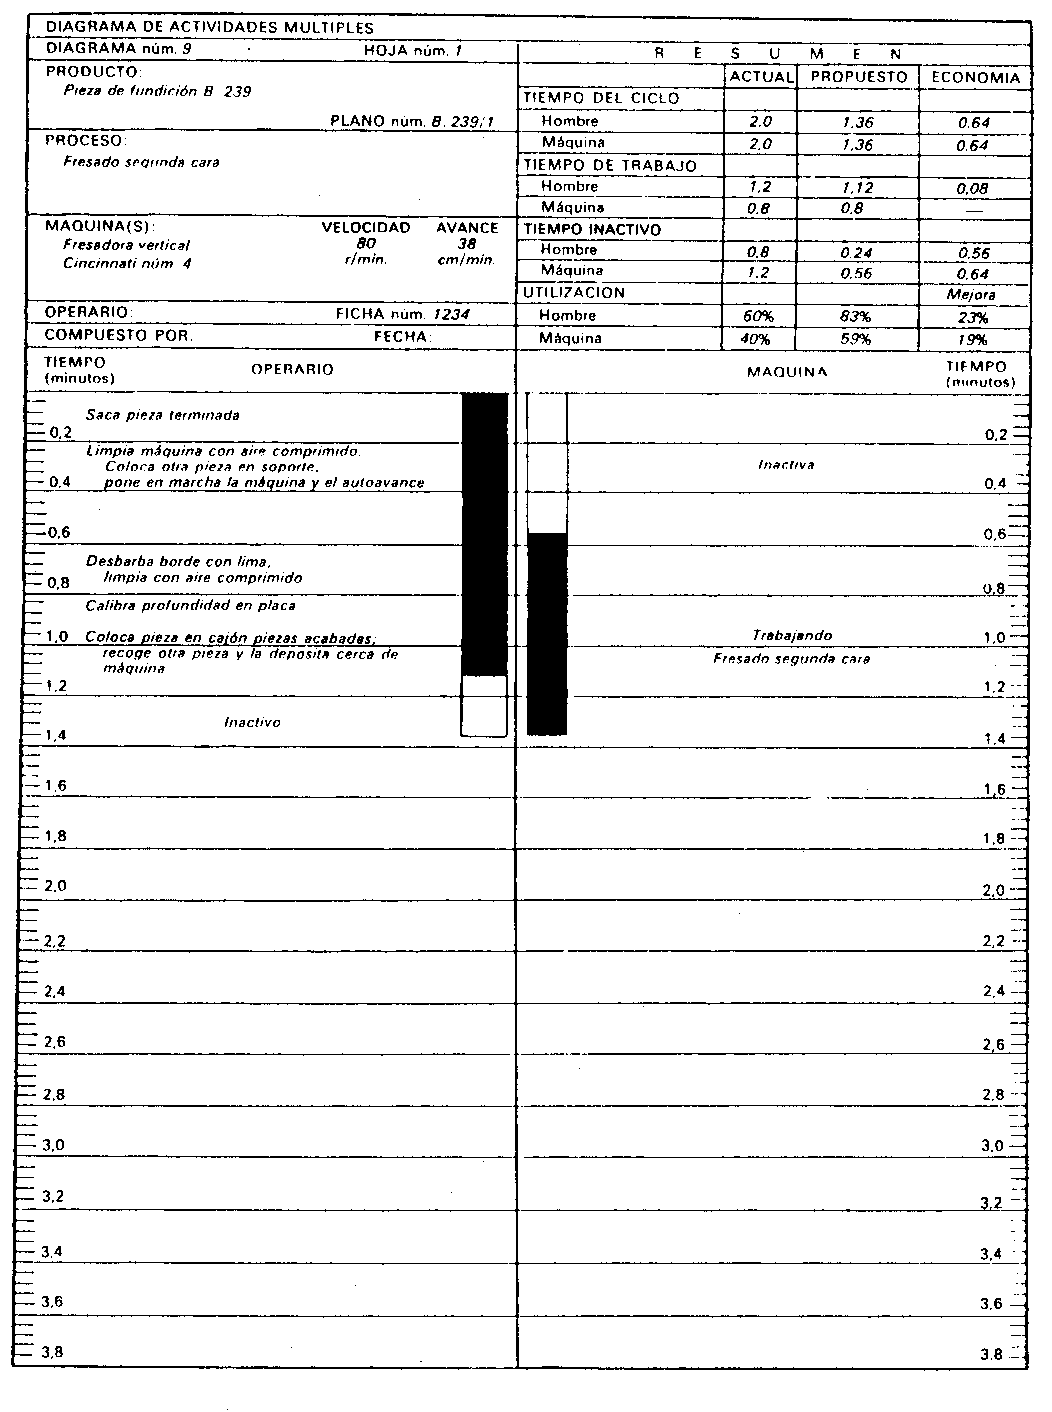
\includegraphics[scale=1.3]{actividades multiples mejorado.png}
    \caption{Diagrama de actividades múltiples 'mejorado'}
    \label{fig:mejorado}
\end{figure}

\begin{figure} [ht!]
    \centering
    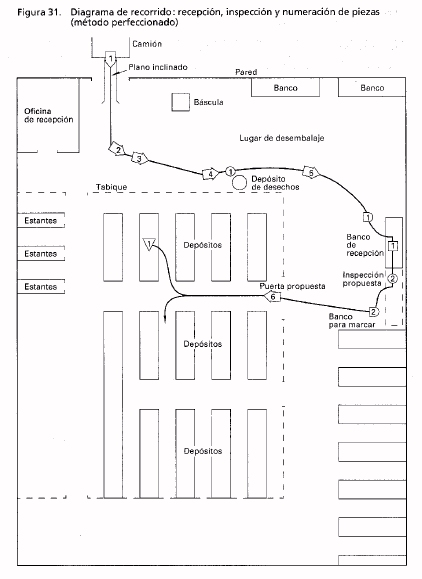
\includegraphics[scale=0.8]{recorrido.png}
    \caption{Diagrama de recorrido}
    \label{fig:recorrido}
\end{figure}

\begin{figure} [ht!]
    \centering
    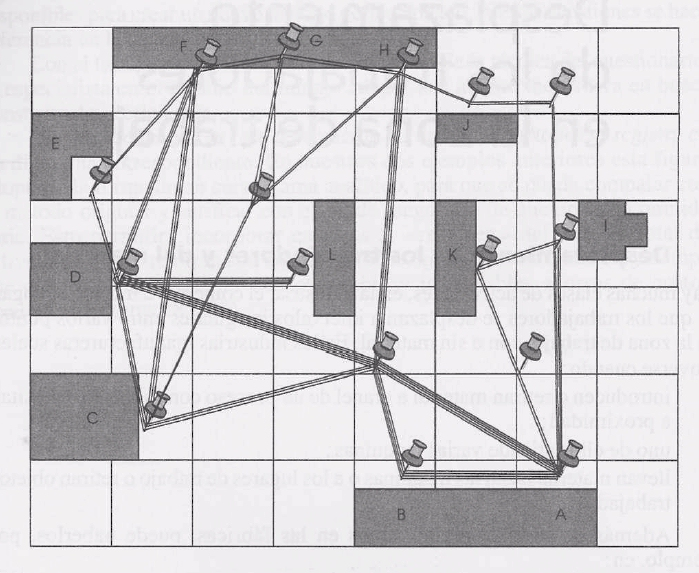
\includegraphics[width=0.5\linewidth]{hilos.png}
    \caption{Diagrama de hilo}
    \label{fig:hilos}
\end{figure}

\begin{figure} [ht!]
    \centering
    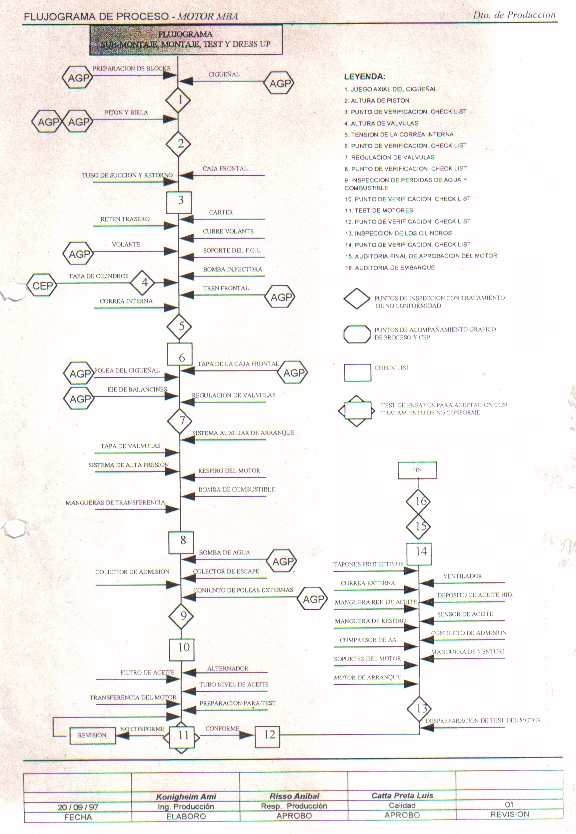
\includegraphics[scale=1.3]{hojaruta.png}
    \caption{Hoja de ruta}
    \label{fig:hojaruta}
\end{figure}

\begin{figure} [ht!]
    \centering
    \rotatebox{90}{\includegraphics[scale=.85]{hoja de proceso.png}}
    \caption{Hoja de proceso}
    \label{fig:hoja de proceso}
\end{figure}

\begin{figure} [ht!]
    \centering
    \rotatebox{90}{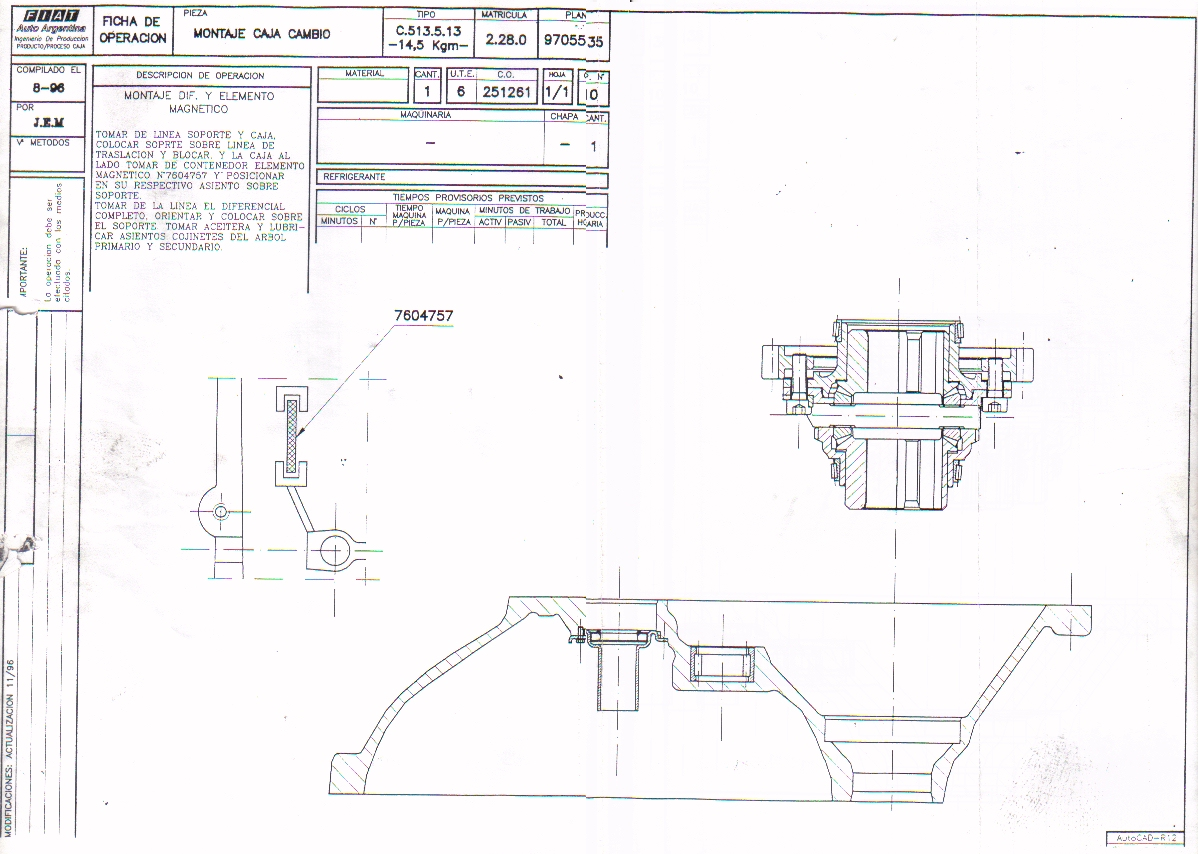
\includegraphics[scale=.85]{ficha de operacion.png}}
    \caption{Ficha de operación}
    \label{fig:ficha de operacion}
\end{figure}


\clearpage

\section{MEDICIÓN DEL TRABAJO}

\subsection{Definción, necesidad, objetivos}

La medición del trabajo es una técnica utilizada para determinar el tiempo requerido por un trabajador calificado para completar una tarea específica, ejecutándola conforme a un método preestablecido y bajo condiciones normales de operación.

El objetivo es: 
\begin{enumerate}
    \item Eliminar tiempos improductivos: Identificar y reducir actividades que no aportan valor al proceso productivo, minimizando demoras, esperas y movimientos innecesarios.
    \item Comparar la eficacia de distintos métodos: Evaluar y contrastar diferentes enfoques para realizar una tarea, determinando cuál ofrece el mejor equilibrio entre eficiencia, calidad y esfuerzo requerido.
    \item Equilibrar líneas de producción: Optimizar la distribución de las cargas de trabajo entre operarios y máquinas, reduciendo cuellos de botella y evitando tiempos ociosos. Un correcto balanceo mejora el flujo de producción y la utilización de los recursos disponibles.
    \item Fijar "tiempos tipo": Establecer estándares de ejecución para cada operación, asegurando que las actividades se realicen dentro de parámetros previsibles y controlados. Esto facilita la planificación, programación y control de la producción.
    \item Imputar costos de mano de obra al producto: Determinar con precisión el tiempo requerido para la fabricación de un producto, permitiendo una asignación adecuada de costos laborales y facilitando la toma de decisiones en materia de precios, presupuestos y rentabilidad.
\end{enumerate}

En síntesis, la medición del trabajo no solo contribuye a mejorar la eficiencia operativa, sino que también proporciona información fundamental para la planificación, el control de costos y la optimización de los recursos en cualquier entorno productivo

Las técnicas para determinar el tiempo son: 

\begin{enumerate}
    \item Muestreo de trabajo: Consiste en la toma de muestras estadísticas y observaciones aleatorias para determinar la frecuencia con la que ocurre una determinada actividad. Su enfoque probabilístico permite obtener resultados representativos con un número reducido de observaciones, siendo útil en entornos con alta variabilidad operativa.
    \item Estimación: Basada en la experiencia del analista, esta técnica subjetiva se emplea para prever el tiempo requerido en actividades futuras. Su precisión depende del conocimiento y juicio del evaluador, por lo que es utilizada en casos donde no se dispone de datos históricos o mediciones directas.
    \item Estudio de tiempos: Método de medición directa y objetiva en el que se cronometra la ejecución de una tarea en condiciones controladas. Se realiza mediante el uso de instrumentos como cronómetros o sistemas electrónicos, registrando el tiempo empleado en cada elemento de la operación. Este enfoque es fundamental para establecer estándares precisos y mejorar la eficiencia operativa.
    \item Normas predeterminadas: Consiste en la asignación de tiempos "modulados" a cada actividad a partir de bases de datos normalizadas. Estos valores son obtenidos de estudios previos y aplicados según el tipo de tarea realizada. Este enfoque permite calcular tiempos sin necesidad de mediciones en planta, facilitando la planificación y evaluación de procesos.
\end{enumerate}

El procedimiento básico para la medición del trabajo, es:

\begin{itemize}
    \item \textbf{Seleccionar:} elegir la tarea a analizar, teniendo en cuenta los aspectos: económicos, técnicos/tecnológicos, humanos, legales/normativos. Las tares se seleccionan con un estudio realizado anteriormente. Ellas son: novedades en la tarea, cambio de material o método, quejas de trabajadora, demoras causadas por una operación, fijación de tiempos, bajo rendimiento, comparar ventajas con otro método, costo excesivo.
    \item \textbf{Registrar:} una descripción completa del método, descomponiendo la operación en \textcolor{purple}{elementos}. El registro, lo  podemos llevar a cabo por técnicas de muestreo, estimación, \textcolor{red}{medición directa}, \textcolor{green}{componiendo la tarea por 'módulos' predefinidos}.
    \item \textbf{Examinar:} los datos registrados, y el detalle de los elementos con sentido crítico, para verificar si se utilizan los métodos y movimientos más eficientes, separando los elementos productivos de los improductivos o extraños.
    \item \textbf{Medir:} la cantidad de trabajo de cada elemento, expresándola en tiempo mediante la técnica más apropiada de medición, asegurando precisión y representatividad en los datos obtenidos.
    \item \textbf{Compilar:} el tiempo tipo de la operación, previendo, si el caso fuera estudio de tiempos con cronómetros, los suplementos correspondientes.
    \item \textbf{Definir:} **definir con precisión la serie de actividades y el método de operación a los que corresponde el tiempo computado, y notificar que este será el tiempo tipo, en ficha de operación, para las actividades y métodos especificados.
\end{itemize}

Entonces, la medición del trabajo consiste en efectuar la observación directa de una tarea, aplicando la medición por cronometraje, la posterior valoración según la experiencia del analista, a fin de calcular el tiempo básico, y por último la adición de suplementos de distintas características, lo que permite determinar el tiempo tipo, que sería aquel que le insumiría a un trabajador calificado efectuar la tarea a un ritmo tipo.

La medición del tiempo en una tarea debe realizarse sobre un proceso previamente optimizado, ya que medir tiempos en actividades no mejoradas solo permite comparaciones sin valor práctico. Por ello, primero se deben aplicar mejoras mediante el estudio de métodos y luego proceder a la medición de tiempos óptimos.  

Antes de iniciar un estudio de tiempos, es clave comunicarlo a los capataces y operarios, destacando sus beneficios. Puede surgir resistencia, especialmente en tareas con incentivos elevados, en cuyo caso se recomienda comenzar con actividades menos conflictivas donde los operarios perciban mejoras.  

El analista debe determinar la cantidad de muestras necesarias para obtener resultados estadísticamente representativos y seleccionar operarios cuyo desempeño refleje el promedio de la planta. Además, debe elegir el método de medición más adecuado y contar con los instrumentos necesarios para llevar a cabo el estudio.

\subsection{Definiciones, teorías}

En la práctica se hace distinción entre trabajador representativo y trabajador calificado. El representativo es aquel cuya competencia y desempeño corresponde al promedio del grupo estudiado, lo que no coincide con trabajador calificado, que se define a continuación.
\begin{itemize}
    \item \textbf{Trabajador calificado:} \\
    Se define como trabajador calificado a aquel individuo que posee las \textcolor{purple}{aptitudes físicas necesarias}, la \textcolor{purple}{inteligencia e instrucción} requeridas y que ha adquirido la \textcolor{purple}{destreza y conocimientos} específicos para ejecutar una tarea conforme a \textcolor{purple}{normas establecidas de seguridad, cantidad y calidad}.  
\end{itemize}


No se trata de un operario excepcionalmente hábil ni de uno con rendimiento promedio, sino de aquel que representa un estándar óptimo dentro de su función.

Seleccionado el trabajador, el analista debe explicarle cuidadosamente, junto a su capataz/jefe, el fin del estudio, y lo que hay que hacer. Se le pedirá que trabaje al ritmo habitual, haciendo las pausas habituales, y mostrando las dificultades del proceso. Es importante evitar el 'vigilar' a la persona, ya que bajo presión, el operario puede alterar su actividad/comportamiento. De ninguna manera se debe cronometrar al operario sin su consentimiento, o a 'espaldas'. \textcolor{red}{NO HAY NADA QUE OCULTAR EN EL ESTUDIO.}

\begin{itemize}
    \item \textbf{Tiempo tipo:} \\
    El tiempo tipo es el tiempo total requerido para la ejecución de una tarea cuando esta se realiza a un ritmo tipo, es decir, bajo condiciones normalizadas de desempeño por parte de un trabajador calificado y siguiendo un método optimizado conforme a estándares preestablecidos de seguridad, calidad y eficiencia

    \item \textbf{Ritmo tipo:} \\
    Corresponde a la idea del ritmo que el analista  se ha formado mentalmente (subjetivamente) al ver cómo trabajan naturalmente los \textcolor{red}{trabajadores calificados} cuando utilizan el método que corresponde y se les ha dado motivo para querer aplicarse (generalmente el  salario).

    El analista debe tener un amplio conocimiento de la tarea que deberá medir, a fin de que su apreciación (valoración) resulte justa. Es por ello que la aplicación de este método requiere de una alta capacitación previa, y - tal como se advierte en la bibliografía -, no ser empleada profesionalmente por personal no calificado. 

    \begin{figure} [ht!]
        \centering
        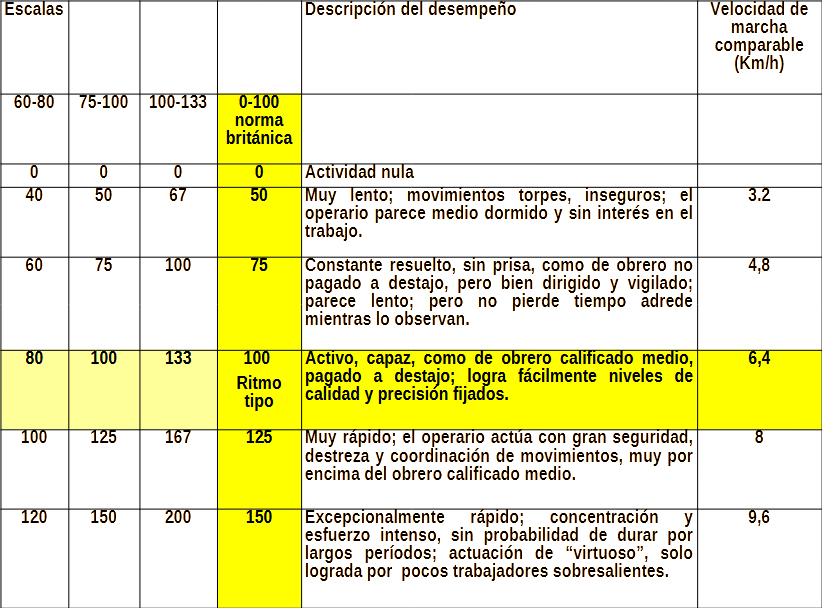
\includegraphics[scale=.55]{ritmo tipo.png}
        \caption{Ritmo tipo}
        \label{fig:enter-label}
    \end{figure}
    
    El ritmo tipo más comúnmente aceptado en los E.E.U.U. y Reino Unido, equivale a la velocidad de movimiento de las extremidades de un hombre de físico corriente que camine sin carga, en terreno llano y en línea recta a 6,4 kilómetros por hora.(dá la impresión de tener un propósito o destino preciso; no se pasea, pero tampoco se apresura).

    \item \textbf{Elemento:} \\
    Es la \textcolor{red}{parte delimitada de una tarea definida}, que se selecciona para facilitar la observación, medición y análisis. Son fácilmente identificables su comienzo y su finalización. Por ejemplo, \textcolor{red}{(corte anterior)} el operario toma (ase) la pieza del contenedor. (el contacto de la mano con la pieza indica el comienzo del elemento). El operario traslada y coloca (suelta) la pieza en la mesa de trabajo . (la separación de la mano de la pieza indica el final del elemento).  \textcolor{red}(corte)

    \begin{figure} [ht!]
        \centering
        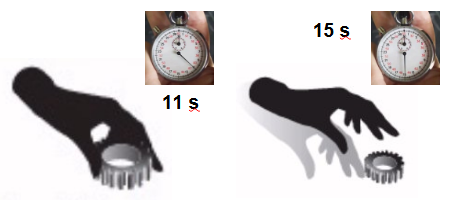
\includegraphics[scale=1]{elemento.png}
        \caption{TIEMPO MEDIDO DEL ELEMENTO: 15 s – 11 s = 4 s}
    \end{figure}

    Existen distintos tipos de elementos:
    \begin{enumerate}
        \item \textbf{Repetitivos:} son aquellos que reaparecen en cada ciclo del trabajo estudiado. (Poner la pieza terminada en otro lugar)
        \item \textbf{Casuales:} reaparecen el cada ciclo de trabajo de manera regular como irregular. Se incorporan al tiempo tipo definitivo. (Ajustar un componente de la máquina)
        \item \textbf{Constante: } son aquellos cuyo tiempo básico de ejecución es siempre igual. (Realizar una medición, torquear tornillo)
        \item \textbf{Variable: } son aquellos cuyo tiempo básico varia según las características del producto, equipo, proceso...
        \item \textbf{Manuales: } las que realiza el trabajador.
        \item \textbf{Mecánicos: } son los realizados automáticamente por las máquinas. (Plegar una lámina de acero)
        \item \textbf{Dominantes: }son los que duran mas tiempo que cualquiera de los demás elementos realizados simultáneamente. (Calentar el agua, mientras armamos el mate)
        \item \textbf{Extraños: }son los observados durante el estudio, pero no son necesarias para realizar la tarea. (Desengrasar una pieza que todavía no se terminó de maquinar)
    \end{enumerate}

    \item \textbf{Valoración:}\\
    Consiste en determinar, a partir de la observación del tiempo que invierte realmente el operario - tiempo observado -, cuál es el tiempo tipo que el trabajador calificado medio puede mantener, y que sirva de base realista para la planificación, el control y los sistemas de primas.
    
    \begin{equation*}
    \text{Valoración} = \dfrac{\text{Tiempo observado x Valor del ritmo observado}}{Valor del ritmo tipo}
    \end{equation*}

    Existen dos casos:
    
    \begin{enumerate}
        \item \textbf{Valoración para desempeño superior a lo normal:}\\
        \begin{figure} [ht!]
            \centering
            \includegraphics[scale=.6]{desempeño uperior.png}
        \end{figure}
        
        Se “demerita” (alarga), ya que debe llevarse a un valor justo para todos. A juicio del analista, el operario efectúa la tarea más rápido de lo habitual
        
        \item \textbf{Valoración para desempeño inferior a lo normal:} \\
        \begin{figure}[ht!]
            \centering
            \includegraphics[scale=.6]{desempeño inf.png}
        \end{figure}
        
        Se “amerita” (acorta), por el mismo motivo anterior. A juicio del analista, el operario efectúa la tarea  más lento a lo habitual

    \end{enumerate}
    

    \item \textbf{Tiempo básico:}\\
    Es el que se tarda en efectuar un elemento de trabajo al ritmo tipo.

    \item \textbf{Suplementos:}\\
    Aún habiendo ideado el método más práctico, económico y eficaz, la tarea continuará exigiendo un esfuerzo humano, por lo que hay que prever ciertos suplementos para compensar la fatiga y descansar. También deben adicionarse suplementos de tiempo para que el trabajador pueda ocuparse de sus necesidades personales, y algunos otros (por ejemplo, por contingencias), para establecer el contenido de trabajo. Ver figura \ref{fig:suplementos}.
    
    \begin{figure} [ht!]
        \centering
        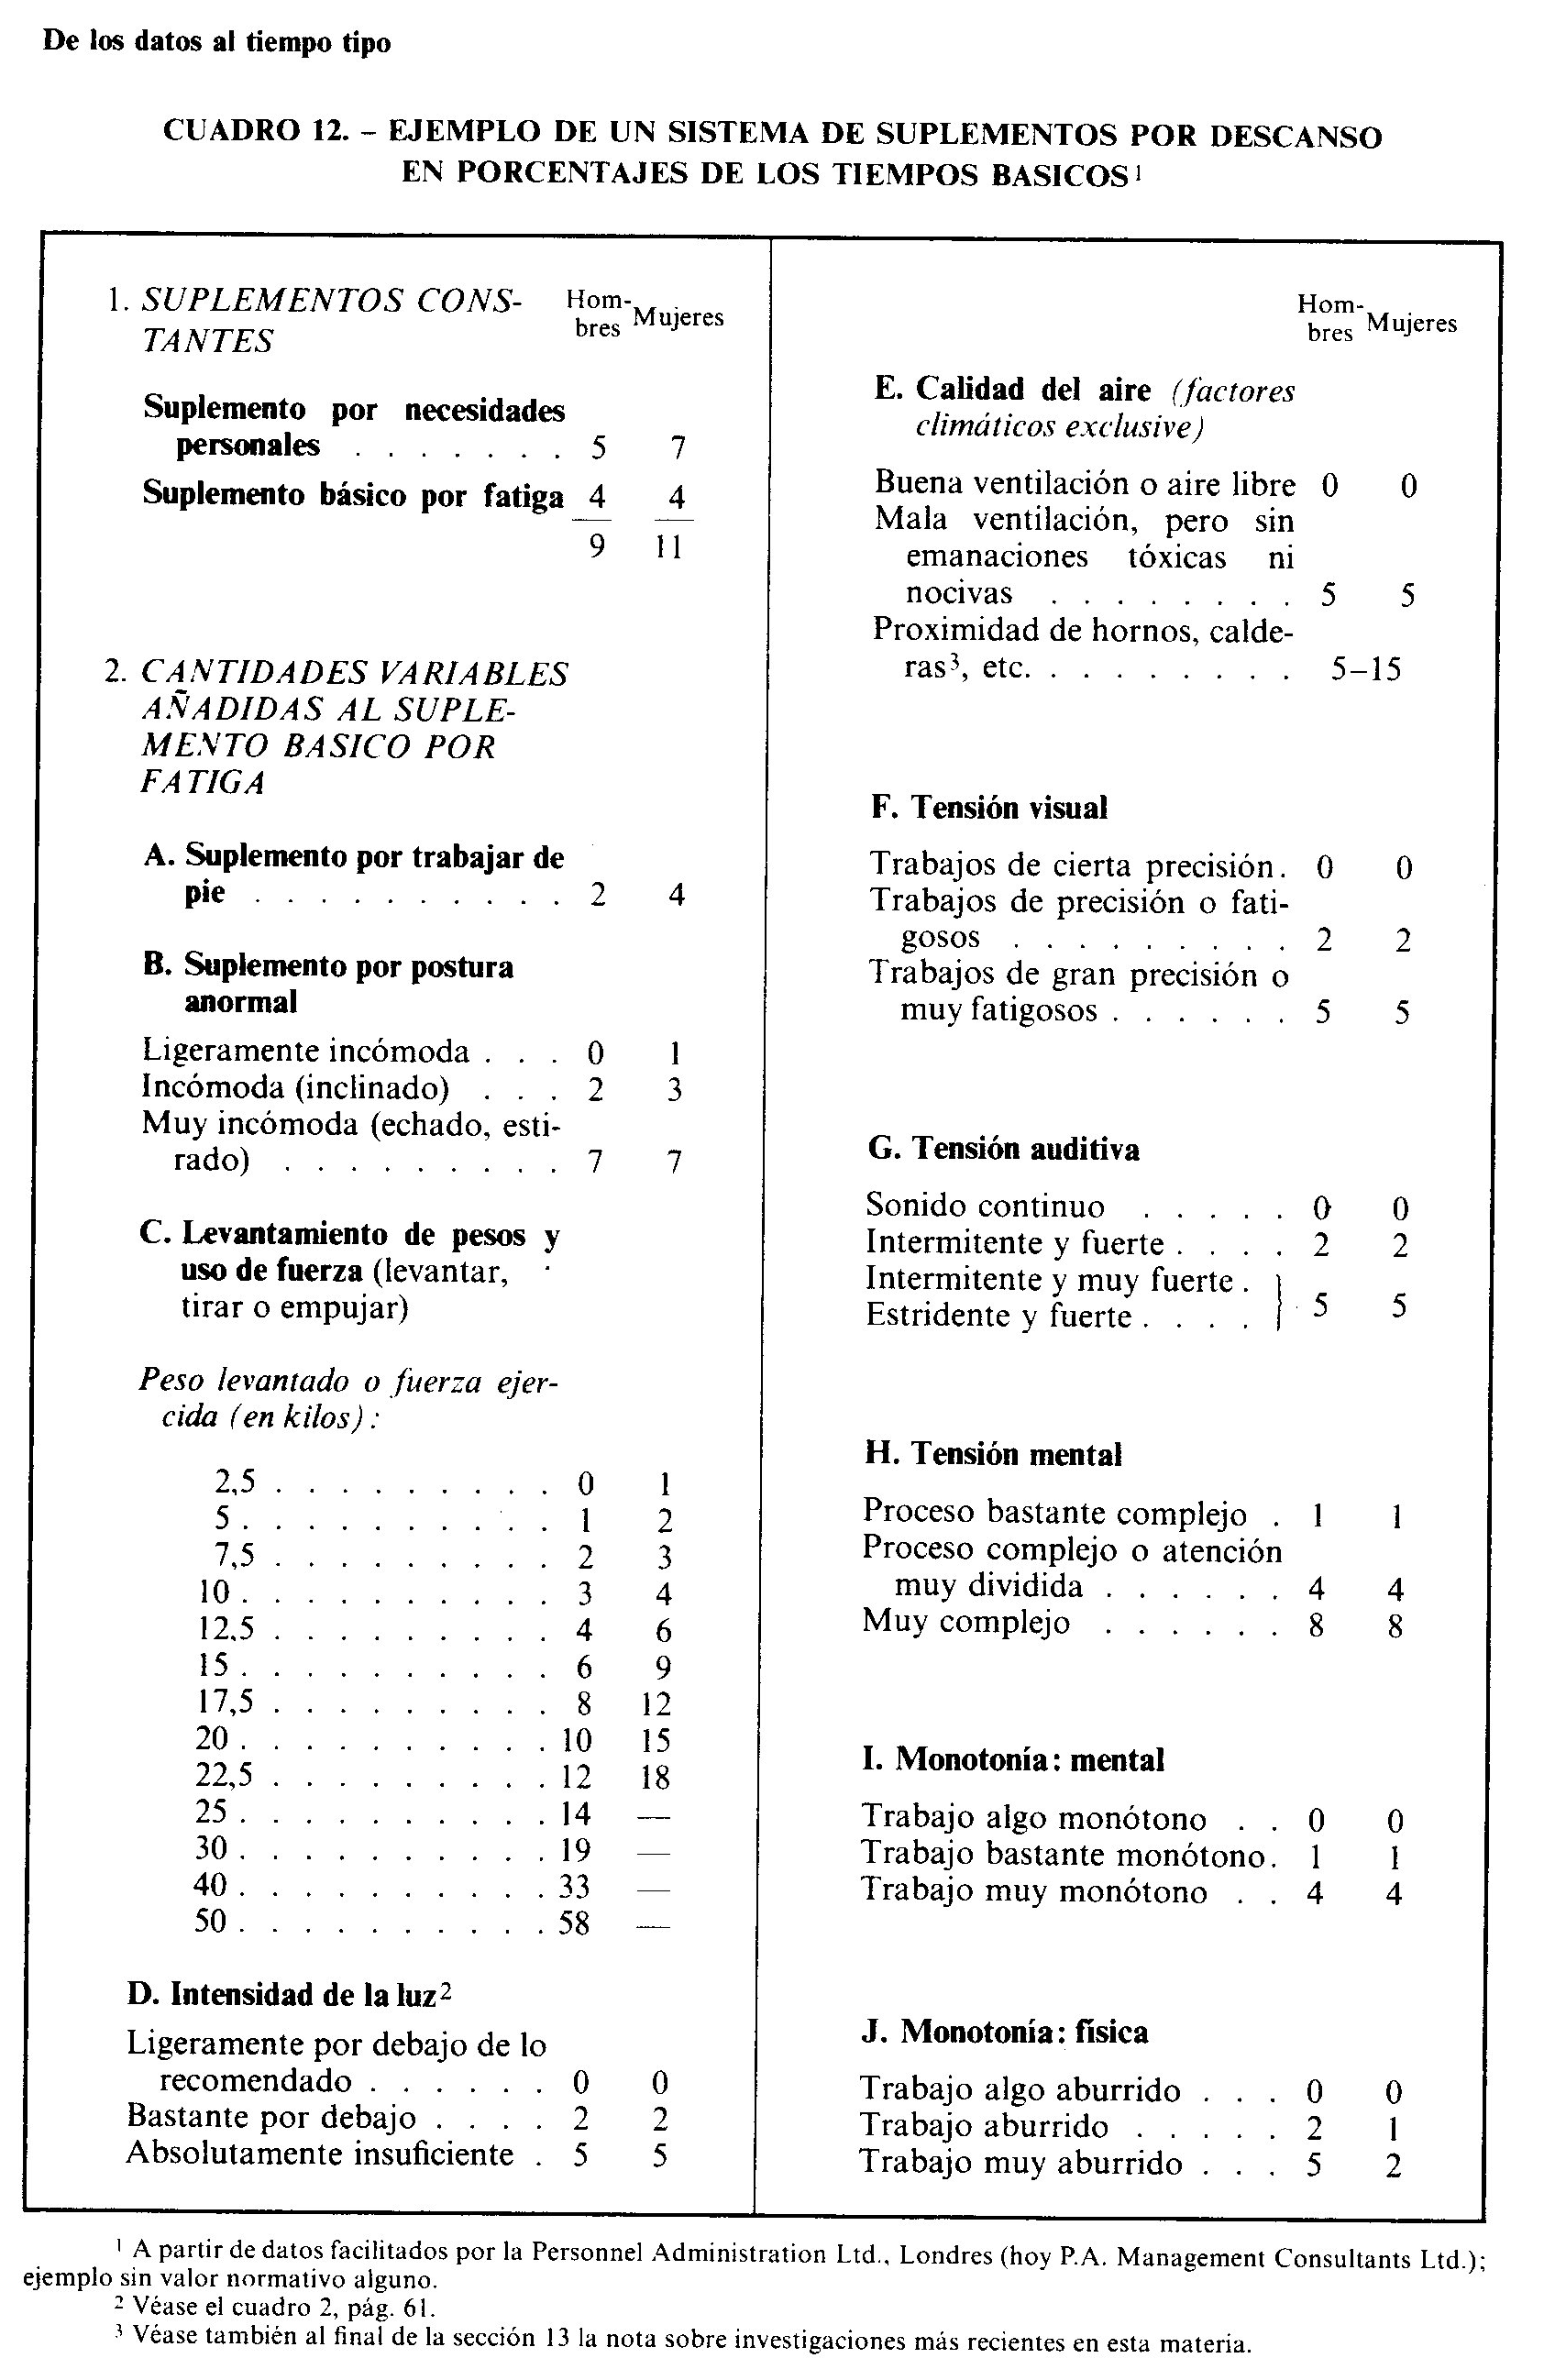
\includegraphics[scale=0.22]{suplementos.png}
        \caption{Suplementos en porcentajes}
        \label{fig:suplementos}
    \end{figure}

    \item \textbf{Definición completa de MEDICIÓN DEL TRABAJO}\\
    Consiste en efectuar la observación directa de una tarea, aplicando la medición por cronometraje -, la posterior valoración -, según la experiencia del analista -, a fin de calcular el tiempo básico, y por último la adición de suplementos de
    distintas características, lo que permite determinar el tiempo tipo, que sería aquel que le insumiría a un trabajador calificado efectuar la tarea a un rítmo tipo.

    \begin{figure} [ht!]
        \centering
        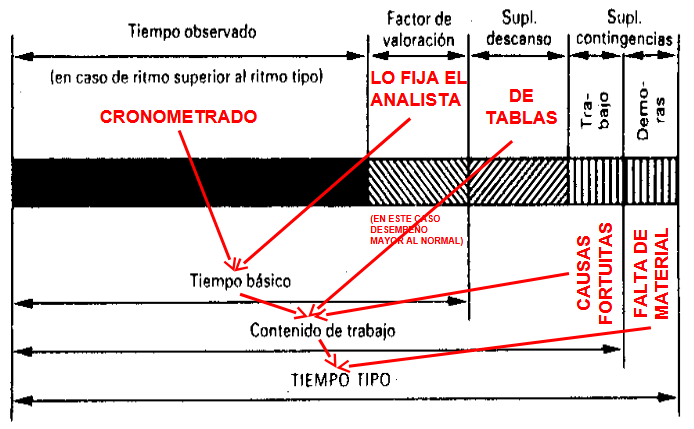
\includegraphics[scale=0.8]{tiempo tipo.png}
        \caption{Enter Caption}
        \label{fig:tiempo tipo}
    \end{figure}
    
\end{itemize}



\subsection{Tipos de cronometraje}

Existen dos procedimientos principales para tomar el tiempo con cronómetro:

    \begin{itemize}
        \item Cronometraje acumulativo: el reloj funciona de modo ininterrumpido durante todo el estudio; se pone en marcha al principio del primer elemento del primer ciclo y no se lo detiene hasta acabar el estudio. Al final de cada elemento se apunta la hora que marca el cronómetro, y los tiempos de cada elemento se obtienen haciendo las respectivas restas después de terminar el estudio. Con este procedimiento se obtiene la seguridad de registrar todo el tiempo en que el trabajo está sometido a observación. Es - en general -, el más preferido.
        \item Cronometraje con vuelta a cero: Los tiempos se toman directamente: al acabar cada elemento se hace volver el segundero a cero y se lo pone de nuevo en marcha inmediatamente, para cronometrar el elemento siguiente, sin que el mecanismo del reloj se detenga ni un momento. (acumula errores de retroceso) tiene la ventaja de que no es necesario efectuar tantas operaciones para determinar los tiempos de cada elemento.
    \end{itemize}


\subsection{Tamaño de la muestra}

Cuantas mediciones hacer sobre el mismo elemento? Consiste en calcular un valor promedio representativo para cada elemento. Es decir, determinar el tamaño de la muestra o el número de observaciones que deben efectuarse para cada elemento, dado un nivel de confianza y un margen de exactitud predeterminados. Se pueden utilizar métodos estadísticos o tradicionales.

Se efectuan cierto número de observaciones preliminares (n´) y luego se aplica la fórmula, para un nivel de confianza de 95,45 \% y un margen de error de 5 \%

\begin{equation*}
    n = (\dfrac{40 \sqrt{n' \sum x^{2} - (\sum x)^2}}{\sum x})^2
\end{equation*}

donde n es el tamaño de la muestra que deseamos determianr, n' es el numero de observaciones del estudio pereliminar, x es el valor de cada una de las observaciones. Se suele redondear hacia arriba.

\begin{figure}
    \centering
    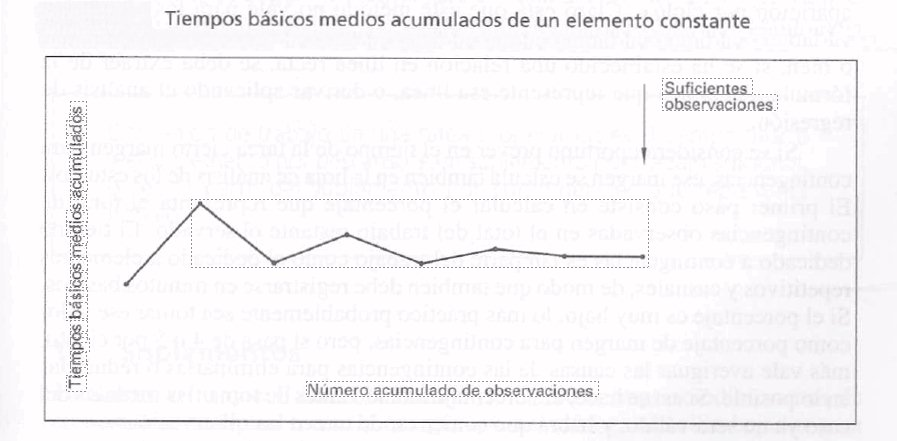
\includegraphics[scale=.5]{convergenica.png}
\end{figure}

Efectuado una cantidad de mediciones según las estadísticamente determinadas (en distintos turnos y horarios), eliminando adicionalmente de las mismas aquellos valores excepcionales (tanto excesivos como muy cortos), y justipreciando por medio de la valoración estimada por el analista, es que puede determinarse un tiempo justo, el cual será representativo del trabajo real del operario.

\subsection{NTPD: Norma de tiempos predeterminados}

La medición por cronómetro tiene las siguientes desventajas:
\begin{itemize}
    \item No se puede realizar hasta que el nuevo método no esté implementado, y se cuente con el operario calificado.
    \item Mala disposicion de operarios y gremios.
    \item Se necesita buen cronometrista.
    \item Falta de objetividad en la valoración.
\end{itemize}

Las NTPD constituyen otro conjunto de técnicas avanzadas que tienen por objeto fijar el tiempo requerido para ejecutar las diferentes actividades, basándose en tiempos previamente establecidos (modulados), para los respectivos movimientos, y no por observación y valorización directas.

Las ventajas de las NTPD:
\begin{itemize}
    \item Evita evaluar la velocidad del operario.
    \item No se altera el ritmo de la empresa.
    \item Se pueden aplicar a tareas que no se están realizando.
    \item Alta aceptación por operarios/gremios.
    \item Menor costo que cronometrar.
    \item Más fiables que los determinados por la empresa.
\end{itemize}

Y las desventajas, son:
\begin{itemize}
    \item Hay actividades / movimientos que no se encuentran en la tabla.
    \item Existen muchos sistemas en uso (dif entre unosy otros).
    \item Falta de unificacion en la unidad de tiempo.
    \item Falta de consideracion entre movimientos precedenmtes y posteriores.
    \item No se consideran factores particulares de la actividad.
    \item No se consideran la dirección de los movimientos.
    \item Para actividades largas, resulta más costosos que cronometrar.
\end{itemize}

Los niveles de cada sistema dependen del grado de detalle que presenta cada uno. Por ejemplo:
\begin{enumerate}
    \item 1er. Nivel, podría discriminar en: soltar, estirar el brazo, asir, trasladar, colocar y soltar. 
    \item 2do. Nivel: recoger y poner.
    \item 3er. Nivel: manipular. 
    \item Para niveles superiores no existen reglas totalmente definidas.
\end{enumerate}

El operario estira el brazo hasta la arandela, la agarra, la traslada hasta el tornillo, la coloca en el tornillo y la suelta

\begin{figure} [ht!]
    \centering
    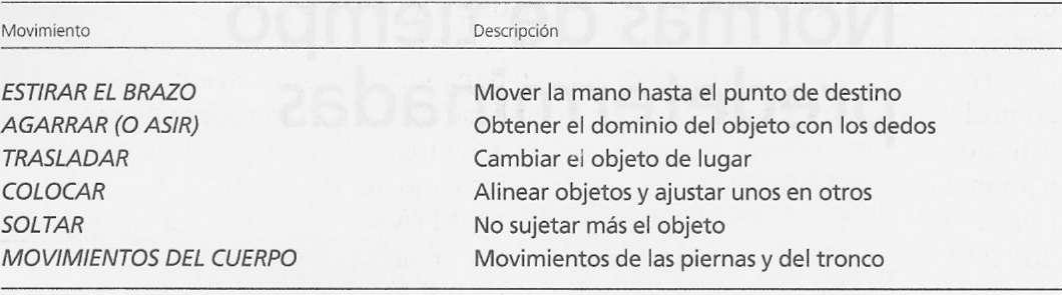
\includegraphics[scale=.65]{movimientos.png}
\end{figure}

Los sistemas son:

\begin{figure} [ht!]
    \centering
    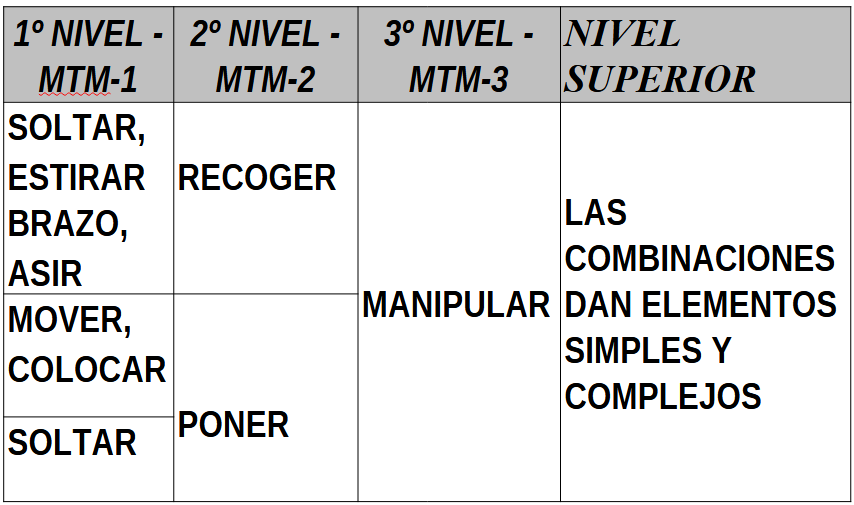
\includegraphics[width=0.6\linewidth]{mtm.png}
\end{figure}

\subsubsection{Sistema MTM-1}

Está compuesto por los siguientes movimientos elementales (tabulados):
\begin{itemize}
    \item ALCANZAR, (R – REACH)
    \item  ALCANZAR, (R – REACH)
    \item   ASIR, (G – GRASP)
    \item   MOVER, (M – MOVE)
    \item   SOLTAR, (RL – RELEASE)
    \item   POSICIONAR, (P – POSITION)
    \item   APLICAR PRESIÓN, (AP – APPLY PRESSURE)
    \item   DESMONTAR, (D – DISENGAGE)
    \item   ROTAR, (T – TURN)
    \item    MOVIMIENTOS DEL CUERPO, (FM, SS, W, ETC.)
    \item   GIRAR MANIVELA, (C – CRANK) 
    \item   ACTIVIDADES DE LA VISTA: (ET Y EF – EYE TRAVEL Y EYE FOCUS)
    \item   MOVIMIENTOS SIMULTÁNEOS (COMBINACIÓN DE LOS ANTERIORES). EN TABLA DE DOBLE ENTRADA
\end{itemize}

La unidad de tiempo es el T.M.U. (unidad de medida de tiempos), equivalente a una hora dividida en 100 000.

\begin{figure} [ht!]
    \centering
    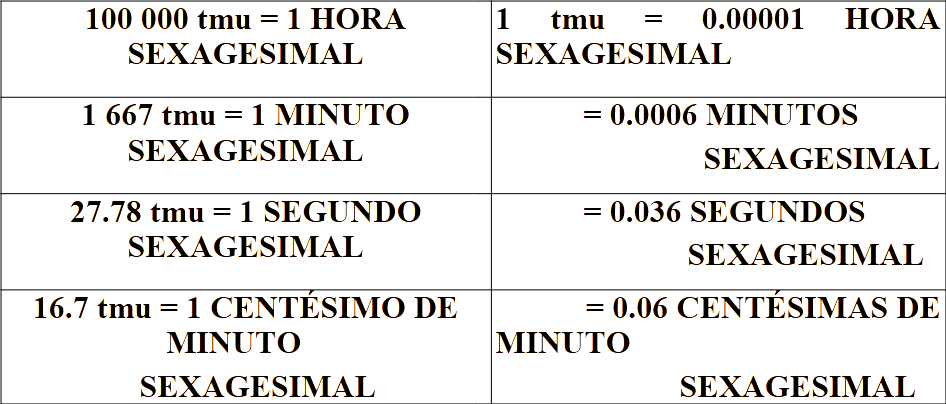
\includegraphics[width=0.5\linewidth]{tmu.png}
\end{figure}


EJEMPLO DE TABLA (ACCIÓN: MOVE): Mover un objeto que pesa 1.5 [kgf], hasta un lugar aproximado ubicado a 55 [cm]


\begin{figure} [ht!]
    \centering
    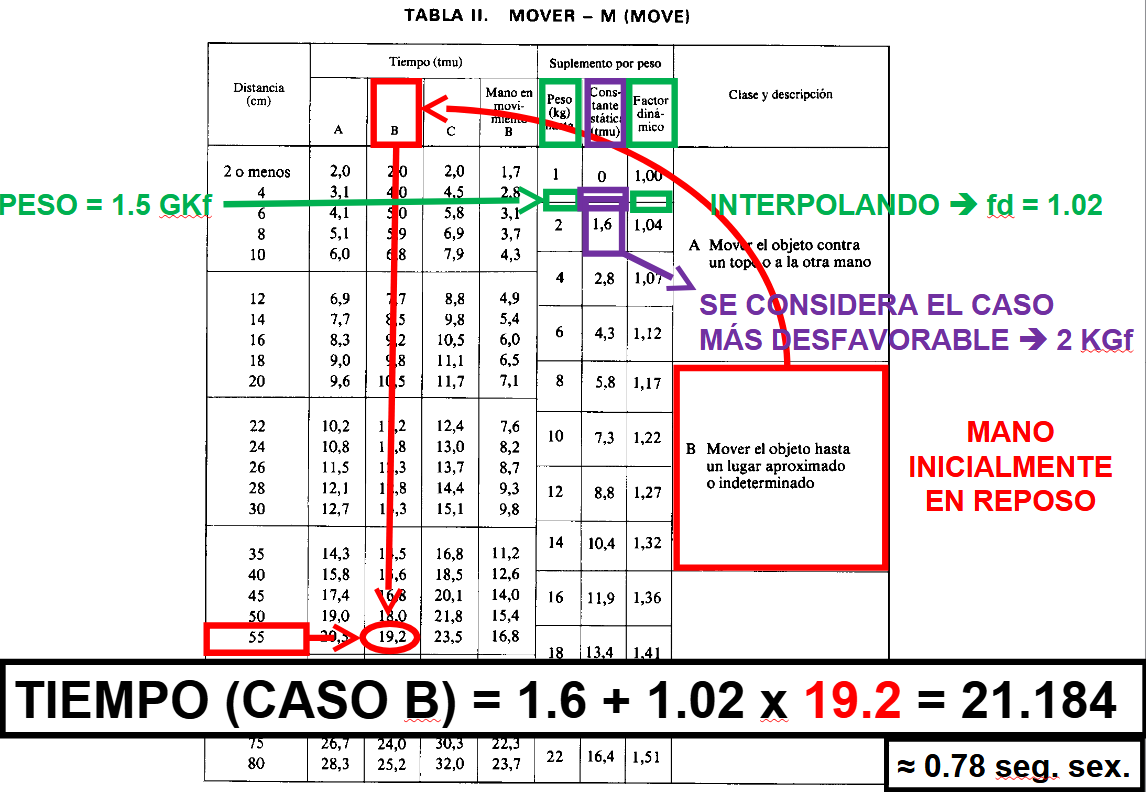
\includegraphics[scale=.38]{ejemplo mover 1.png}
\end{figure}


\begin{figure} [ht!]
    \centering
    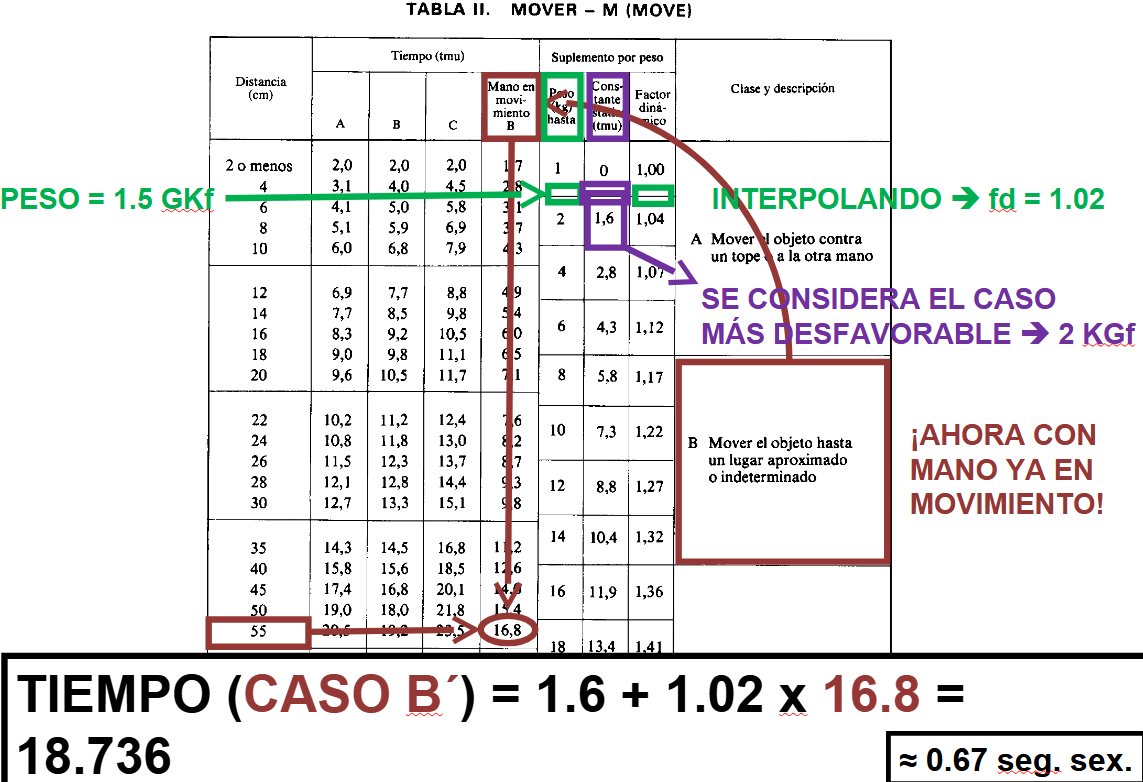
\includegraphics[scale=.5]{ejemplo mover 2.png}
\end{figure}

\clearpage

\clearpage


\section{Capítulo 5: Mantenimiento Industrial}

El objetivo del mantenimiento industrial es lograr el máximo nivel de efectividad en el funcionamiento de un sistema productivo o de servicios, garantizando la menor contaminación ambiental, la mayor seguridad para el personal y el mínimo costo operativo posible.

El mantenimiento industrial no se limita exclusivamente a las máquinas, sino que también incluye el cuidado y conservación de las instalaciones: sistemas de iluminación, redes de computación, energía eléctrica, aire comprimido, agua, aire acondicionado, calles internas, pisos y depósitos.

\subsection{Criterios para definir el mantenimiento:}
En sectores como el aeronáutico y el militar, donde la confiabilidad y la eficiencia son críticas, se aplican enfoques avanzados que priorizan la planificación estratégica del mantenimiento. Estos enfoques se basan en dos pilares fundamentales:
\begin{enumerate}
    \item CBM – Condition Based Maintenance (Mantenimiento Basado en la Condición):

    Es una estrategia de mantenimiento que no se basa en intervalos fijos de tiempo, sino en el estado real del equipo. Para ello, se utilizan sensores y sistemas de monitoreo que analizan variables clave (vibraciones, temperatura, consumo eléctrico, etc.) en tiempo real.
    \begin{itemize}
        \item El mantenimiento se ejecuta solo cuando los indicadores muestran signos de deterioro o desgaste, evitando intervenciones innecesarias y reduciendo riesgos de falla.

        \item Ejemplo: Si un motor muestra aumento en vibraciones fuera de lo normal, se programa una intervención antes de que ocurra una avería.
    \end{itemize}
    \item System Effectiveness and Control of the Program Life-Cycle Costs (Efectividad del Sistema y Control de Costos durante el Ciclo de Vida)

    Este enfoque apunta a maximizar el rendimiento total del sistema desde su adquisición hasta su retiro, considerando todos los costos involucrados: instalación, operación, mantenimiento, repuestos, actualizaciones y disposición final.
    \begin{itemize}
        \item Se enfoca en tomar decisiones de mantenimiento que resulten rentables a largo plazo, no solo en lo inmediato. El objetivo es lograr la mayor eficiencia operativa con el menor costo total durante toda la vida útil del equipo.
        \item Ejemplo: Elegir una bomba más costosa al inicio, pero que requiera menos mantenimiento y consuma menos energía, puede ser más conveniente a lo largo del tiempo.
    \end{itemize}
\end{enumerate}

\begin{figure} [ht!]
    \centering
    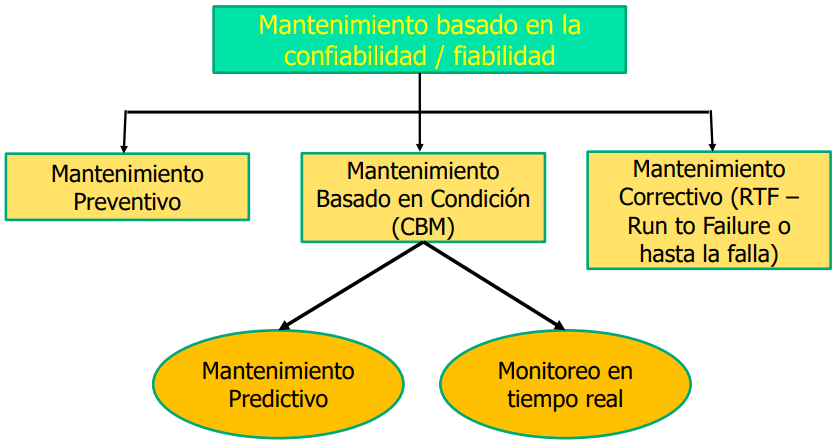
\includegraphics[scale=0.47]{mantenimiento.png} 
\end{figure}

\subsection{Fiabilidad:}

Entendemos como fiabilidad (representada como Rj, del inglés reliability) de un equipo o sistema a la probabilidad de que cumpla su función sin fallas durante un período de tiempo determinado y bajo condiciones específicas de operación.
\begin{itemize}
    \item \textbf{Valor = 1} $\rightarrow$ indica que el sistema es fiable en un 100\%
    \item \textbf{Valor = 0} $\rightarrow$ indica que el sistema NO es fiable – 0\%
\end{itemize}

Cuando un sistema está compuesto por varios elementos o subsistemas, la fiabilidad global dependerá de cómo están interconectados: en serie o en paralelo.

\begin{itemize}
    \item Fiabilidad en serie
    Se aplica cuando todos los componentes deben funcionar correctamente para que el sistema global funcione. Su fórmula:

    \begin{equation*}
        R_{s} = R_{1} \cdot R_{2} \cdot ... \cdot R_{n}
    \end{equation*}

    La fiabilidad total del sistema disminuye a medida que se agregan componentes, ya que el fallo de uno solo implica el fallo del sistema completo.

    Las ventajas son: simplicidad en el diseño y el análisis, costos iniciales menores (sin redundancias)

    Las desventajas son: baja tolerancia a fallos, el sistema es tan fiable como su componente más débil, mayor riesgo de interrupción total.

    \item Fiabilidad en paralelo:
    Se aplica cuando el sistema puede continuar funcionando mientras al menos uno de los componentes siga operativo. Su fórmula: 

    \begin{equation*}
        R_{s} = 1 - [(1-R_{1}) \cdot (1-R_{2}) \cdot ... \cdot (1-R_{n})]
    \end{equation*}

    La fiabilidad en paralelo aumenta considerablemente la fiabilidad global, ya que la redundancia permite tolerancia a fallas.

    Las ventajas son: alta disponibilidad del sistema, mayor robustez frente a fallos individuales, ideal para sistemas críticos (aeronáutica, medicina, energía).

    Las desventajas son: mayor complejidad de diseño y mantenimiento, costos iniciales y operativos más altos.
    
\end{itemize}

\textit{Advertencia! En un sistema con componentes en paralelo y en serie hay que resolver primero los componentes en paralelo y luego la serie (como en los circuitos electrónicos, eléctricos).}

\subsection{Aspectos estratégicos y tácticos de Mantenimiento}

\begin{enumerate}
    \item \textit{Definir el Sistema de Mantenimiento:}

    Estrategia: Define cómo se va a enfrentar el deterioro natural de los equipos y qué enfoque se tomará ante las fallas.

    Táctica: Permite planificar intervenciones (paradas, repuestos, tiempos) según el tipo elegido.

    El sistema de mantenimiento de una organización debe estar alineado con los objetivos productivos, el tipo de equipamiento utilizado y los recursos disponibles. Existen diversas estrategias que pueden implementarse de manera combinada para maximizar la disponibilidad y confiabilidad de los activos:
    \begin{itemize}
        \item \textbf{Mantenimiento Correctivo:}

        Consiste en reparar el equipo una vez ocurrido el fallo. Se utiliza generalmente en equipos no críticos, donde las paradas no afectan significativamente la producción.
        
        Las ventajas:
        \begin{itemize}
            \item Costos iniciales bajos.
            \item No requiere planificación compleja.
        \end{itemize}
        Las desventajas:
        \begin{itemize}
            \item Paradas imprevistas.
            \item Riesgo de daños mayores o accidentes.
            \item Impacto negativo en la producción.
        \end{itemize}
        
        \textit{Ejemplo: Una cinta transportadora en la línea de ensamblado se detiene de forma inesperada por una falla en el motor. El equipo de mantenimiento interviene una vez ocurrido el fallo, reemplazando el motor dañado y reanudando la operación. Este tipo de mantenimiento no estaba planificado.}
        
        \item \textbf{Mantenimiento Preventivo:}

        Consiste en intervenciones programadas según el tiempo o el uso, sin esperar a que ocurra una falla. Ideal para equipos con desgaste conocido o cuya falla afecte la seguridad o el proceso.

        Las ventajas:
        \begin{itemize}
            \item Reducción de fallas imprevistas.
            \item Mejora la vida útil del equipo.
        \end{itemize}
        Las desventajas:
        \begin{itemize}
            \item Puede realizarse mantenimiento innecesario.
            \item Mayor consumo de repuestos y mano de obra si no está optimizado.
        \end{itemize}

        \textit{Ejemplo: Cada tres meses, el equipo técnico realiza el cambio de filtros y lubricación en todas las prensas hidráulicas, independientemente de si presentan fallas o no. El objetivo es evitar que fallen por desgaste o acumulación de contaminantes.}

        \item \textbf{Mantenimiento Predictivo:}

        Se basa en el monitoreo de condiciones operativas (vibraciones, temperatura, ruido, etc.) para predecir cuándo ocurrirá una falla. Ideal para equipos críticos donde conviene anticipar el fallo para planificar la intervención.

        Las ventajas:
        \begin{itemize}
            \item Intervención solo cuando es necesario.
            \item Disminución de costos por parada no planificada.
        \end{itemize}
        Las desventajas:
        \begin{itemize}
            \item Requiere inversión en sensores y tecnología.
            \item Necesita personal capacitado para análisis de datos.
        \end{itemize}

        \textit{Ejemplo: En una planta de producción, se utilizan sensores de vibración para monitorear los rodamientos de motores eléctricos. Cuando las vibraciones exceden un umbral preestablecido, se programa el cambio del rodamiento antes de que se produzca la falla. El mantenimiento se hace basado en la condición real del equipo.}

        \item \textbf{TPM (Total Productive Maintenance)}

        Estrategia que busca involucrar a todo el personal de la empresa (especialmente a los operarios, no solo al área de mantenimiento) en el cuidado del equipo. Cultura de mejora continua y participación activa de los operadores en el mantenimiento básico.
        
        Las ventajas:
        \begin{itemize}
            \item Mejora la autonomía del operario.
            \item Aumenta la disponibilidad y eficiencia de los equipos.
            \item Fomenta la responsabilidad compartida.
        \end{itemize}
        Las desventajas:
        \begin{itemize}
            \item Requiere fuerte compromiso organizacional
            \item Necesita entrenamiento constante y cambio cultural.
        \end{itemize}

        \textit{Ejemplo: Los operarios de una máquina inyectora realizan diariamente una rutina de limpieza, chequeo de presión, apriete de componentes y reporte de anomalías en una hoja de control visual. Están involucrados directamente en el mantenimiento básico del equipo, lo cual mejora su cuidado y reduce tiempos de parada.}



A continuación, se presenta un resumen: 
\begin{table}[ht!]
\centering
\resizebox{\columnwidth}{!}{%
\begin{tabular}{|l|l|l|l|l|}
\hline
\multicolumn{1}{|c|}{\textbf{\begin{tabular}[c]{@{}c@{}}Tipo de \\ Mantenimiento\end{tabular}}} & \multicolumn{1}{c|}{\textbf{Descripción}}                                                                   & \multicolumn{1}{c|}{\textbf{Objetivo Principal}}                                                              & \multicolumn{1}{c|}{\textbf{Ventajas}}                                                                         & \multicolumn{1}{c|}{\textbf{Desventajas}}                                                                          \\ \hline
\textbf{Correctivo}                                                                             & \begin{tabular}[c]{@{}l@{}}Se realiza después de que\\ ocurre una falla.\end{tabular}                       & \begin{tabular}[c]{@{}l@{}}Restablecer el funcionamiento\\ del equipo.\end{tabular}                           & \begin{tabular}[c]{@{}l@{}}Bajo costo inmediato si\\ el equipo no es crítico.\end{tabular}                     & \begin{tabular}[c]{@{}l@{}}Paradas imprevistas, riesgos\\ operativos, mayores\\ costos a largo plazo.\end{tabular} \\ \hline
\textbf{Preventivo}                                                                             & \begin{tabular}[c]{@{}l@{}}Se programa en intervalos\\ de tiempo o uso.\end{tabular}                        & \begin{tabular}[c]{@{}l@{}}Evitar fallas mediante\\ intervenciones regulares.\end{tabular}                    & \begin{tabular}[c]{@{}l@{}}Disminuye paradas inesperadas,\\ prolonga vida útil.\end{tabular}                   & \begin{tabular}[c]{@{}l@{}}Puede generar mantenimiento\\ innecesario, costo por\\ sobreintervención.\end{tabular}  \\ \hline
\textbf{Predictivo}                                                                             & \begin{tabular}[c]{@{}l@{}}Basado en el monitoreo de\\ condiciones del equipo.\end{tabular}                 & \begin{tabular}[c]{@{}l@{}}Anticipar fallas y actuar\\ justo a tiempo.\end{tabular}                           & \begin{tabular}[c]{@{}l@{}}Máxima eficiencia en intervenciones,\\ reducción de costos por fallas.\end{tabular} & \begin{tabular}[c]{@{}l@{}}Alta inversión inicial, requiere\\ sensores y análisis de datos.\end{tabular}           \\ \hline
\textbf{TPM}                                                                                    & \begin{tabular}[c]{@{}l@{}}Participación activa del personal \\ operativo en el mantenimiento.\end{tabular} & \begin{tabular}[c]{@{}l@{}}Maximizar la eficiencia de\\ los equipos con involucramiento\\ total.\end{tabular} & \begin{tabular}[c]{@{}l@{}}Mejora continua, menor tiempo de\\ inactividad, mayor cuidado.\end{tabular}         & \begin{tabular}[c]{@{}l@{}}Requiere cambio cultural,\\ formación\\ y compromiso organizacional.\end{tabular}       \\ \hline
\end{tabular}%
}
\end{table}

    \end{itemize}
    \item \textit{Gestión del Mantenimiento:}

    Estrategia: Establece objetivos a largo plazo, como la confiabilidad y la disponibilidad de equipos clave.

    Táctica: Permite monitorear tareas, programar mantenimientos, hacer trazabilidad, y tomar decisiones con base en datos.

    La gestión del mantenimiento abarca el conjunto de herramientas, recursos y metodologías necesarias para garantizar que el sistema de mantenimiento funcione de forma eficiente, controlada y alineada con los objetivos de la organización. Se apoya tanto en decisiones estratégicas como en acciones operativas concretas. Entre los ejes principales se destacan:

    \begin{itemize}
        \item \textit{Costos de Mantenimiento:}
        
        Una gestión efectiva requiere identificar, medir y controlar los costos directos e indirectos asociados al mantenimiento. Esto incluye repuestos, mano de obra, herramientas, paradas de planta, y pérdidas por ineficiencia. Un análisis detallado permite tomar decisiones económicas inteligentes, como definir si conviene reparar, reemplazar o actualizar un equipo.

        \item \textit{Gestión de stocks de repuestos:}

        Tener una política de stock bien diseñada es crucial para garantizar la disponibilidad de piezas críticas sin sobredimensionar el inventario. Esto implica clasificar repuestos según su criticidad, determinar puntos de pedido, gestionar proveedores confiables y minimizar los tiempos de reposición. Una mala gestión puede derivar en paradas prolongadas o costos innecesarios por exceso de inventario.

        \item \textit{Tablero de comando:}

        El uso de tableros de control o “dashboards” permite visualizar en tiempo real los principales indicadores de mantenimiento, como el índice de fallas, tiempo medio entre fallas (MTBF), tiempo medio de reparación (MTTR), disponibilidad de equipos y cumplimiento del plan. Es una herramienta de gestión clave para la toma de decisiones basada en datos y el seguimiento de desempeño.

        \item \textit{Organización y administración:}

        Implica estructurar el área de mantenimiento según criterios de eficiencia, jerarquía y responsabilidad. Incluye definir roles, turnos, procedimientos de trabajo, comunicación con otras áreas, y asegurar el cumplimiento de normas de seguridad y calidad. Una buena organización permite reducir tiempos muertos, mejorar la trazabilidad de acciones y aumentar la productividad del área.

        \item \textit{Sistemas informaticos:}

        Actualmente, los sistemas GMAO (Gestión del Mantenimiento Asistido por Ordenador) como SAP PM, Maximo o MaintControl, son herramientas esenciales para planificar, registrar, monitorear y analizar todas las actividades de mantenimiento. Permiten gestionar activos, generar órdenes de trabajo, programar tareas preventivas, controlar costos y generar reportes. Su implementación profesionaliza el área y habilita una gestión basada en datos concretos.
    \end{itemize}
\begin{table}[ht!]
\centering
\begin{tabular}{|l|l|}
\hline
\multicolumn{1}{|c|}{\textbf{Elemento}} & \multicolumn{1}{c|}{\textbf{Descripción Resumida}}                                                                                      \\ \hline
\textbf{Costos de Mantenimiento}        & \begin{tabular}[c]{@{}l@{}}Controlar y optimizar los costos directos \\ e indirectos asociados al mantenimiento.\end{tabular}           \\ \hline
\textbf{Gestión de repuestos}           & \begin{tabular}[c]{@{}l@{}}Asegurar disponibilidad sin sobredimensionar\\ el stock; clasificar y controlar repuestos.\end{tabular}      \\ \hline
\textbf{Tablero de comando}             & \begin{tabular}[c]{@{}l@{}}Visualizar indicadores clave (MTBF, MTTR,\\ disponibilidad) para mejorar la toma de decisiones.\end{tabular} \\ \hline
\textbf{Organización y administración}  & \begin{tabular}[c]{@{}l@{}}Estructurar el área de mantenimiento: roles,\\ turnos, procedimientos y coordinación.\end{tabular}           \\ \hline
\textbf{Sistemas informáticos}          & \begin{tabular}[c]{@{}l@{}}Usar software (GMAO) para planificar, registrar\\ y analizar actividades de mantenimiento.\end{tabular}      \\ \hline
\end{tabular}
\end{table}

    \item \textit{Recursos Humanos:}
    
    Estrategia: Asegura que la empresa cuente con personal capacitado y alineado con los objetivos del mantenimiento.

    Táctica: Define turnos, asigna tareas, asegura cumplimiento de protocolos, y responde eficazmente ante fallas.  

    El capital humano es uno de los pilares fundamentales en cualquier estrategia de mantenimiento. Su correcta gestión permite asegurar la disponibilidad, competencia y motivación del personal técnico, garantizando intervenciones eficientes, seguras y de calidad.

    \begin{itemize}
        \item \textit{Gestión de los Recursos Humanos:}
        
        Involucra la planificación, selección, capacitación y evaluación del personal de mantenimiento. Se busca asegurar que el equipo esté capacitado técnicamente, pero también comprometido con la cultura organizacional y los objetivos estratégicos. Además, implica diseñar esquemas de trabajo adecuados (guardias, turnos, descansos), mantener buen clima laboral y promover la mejora continua.
        
        \item \textit{Especialidades de Mantenimiento:}

        El mantenimiento requiere perfiles técnicos diversos, según el tipo de activos: mecánicos, eléctricos, electrónicos, neumáticos, hidráulicos, instrumentistas, entre otros. La identificación y desarrollo de estas especialidades permite optimizar los recursos humanos y garantizar una respuesta técnica adecuada ante cualquier situación.
        
        \item \textit{Higiene y seguridad:}

        Es indispensable garantizar que todas las tareas de mantenimiento se realicen bajo condiciones seguras, cumpliendo normativas legales y buenas prácticas. Esto incluye:

        \begin{itemize}
            \item Uso de elementos de protección personal (EPP).
            \item Procedimientos seguros (bloqueo y etiquetado, trabajos en altura, atmósferas explosivas).
            \item Capacitaciones periódicas.
            \item Evaluación de riesgos por tarea.
        \end{itemize}

        Una política activa en higiene y seguridad reduce accidentes, protege al personal y evita pérdidas económicas o legales.
    \end{itemize}

\begin{table}[ht!]
\centering
\begin{tabular}{|l|l|}
\hline
\multicolumn{1}{|c|}{\textbf{Elemento}}  & \multicolumn{1}{c|}{\textbf{Descripción Resumida}}                                                                              \\ \hline
\textbf{Gestión de Recursos Humanos}     & \begin{tabular}[c]{@{}l@{}}Planificación, capacitación, evaluación\\ y organización del personal técnico.\end{tabular}          \\ \hline
\textbf{Especialidades de Mantenimiento} & \begin{tabular}[c]{@{}l@{}}Diversificación de perfiles técnicos:\\ mecánicos, eléctricos, electrónicos, etc.\end{tabular}       \\ \hline
\textbf{Higiene y seguridad}             & \begin{tabular}[c]{@{}l@{}}Cumplimiento de normas, uso de EPP,\\ procedimientos seguros y prevención\\ de riesgos.\end{tabular} \\ \hline
\end{tabular}
\end{table}

\end{enumerate}

Analizar los aspectos estratégicos y tácticos del mantenimiento permite comprender cómo se organiza, gestiona y optimiza esta función clave dentro de una empresa industrial. El objetivo es asegurar la disponibilidad, confiabilidad y seguridad de los activos productivos, minimizando costos, evitando fallas y prolongando la vida útil de los equipos.

Este análisis proporciona una visión integral que combina la planificación técnica, la gestión económica, la organización del personal y el uso de herramientas informáticas, todo orientado a mejorar la eficiencia operativa y la competitividad de la empresa.


\subsection{Variables de mantenimiento:}

En el ámbito industrial, el análisis y la gestión eficiente del mantenimiento requieren comprender una serie de variables clave que permiten evaluar el desempeño de los sistemas técnicos. Estas variables constituyen la base para la toma de decisiones estratégicas y operativas, ya que influyen directamente en la efectividad, costos, seguridad, y disponibilidad de los equipos.

Entre las principales variables se encuentran la fiabilidad, la mantenibilidad, la disponibilidad y la durabilidad, cada una de ellas enfocada en aspectos específicos del comportamiento de los activos a lo largo de su ciclo de vida.

\begin{enumerate}
    \item \textit{Fiabilidad:}

    La fiabilidad (Rj) es la probabilidad de que un sistema, instalación, máquina, equipo o componente cumpla su función sin fallar durante un período de tiempo determinado y bajo condiciones específicas de operación.

    \item \textit{Disponibilidad:}

    La disponibilidad de un sistema o equipo se define como la proporción del tiempo durante el cual se encuentra en condiciones operativas, es decir, en condiciones de ser utilizado para cumplir su función.
    \begin{equation*}
        \text{Disponibilidad} = \dfrac{\text{Tiempo de operación}}{\text{Tiempo total programado}} = \dfrac{\text{Tiempo total programado – Tiempo de paradas}}{\text{Tiempo total programado}}
    \end{equation*}

    Esta variable depende de dos factores principales:

    \begin{itemize}
        \item La frecuencia de fallas del sistema.
        \item El tiempo necesario para restaurar el servicio tras una interrupción.
    \end{itemize}

    Una alta disponibilidad es clave en sistemas críticos, ya que garantiza continuidad operativa y eficiencia productiva.

    \item \textit{Mantenibilidad:}

    La mantenibilidad es la probabilidad de que un equipo o sistema pueda ser reparado y restituido a una condición operativa específica dentro de un período de tiempo determinado, siempre que el mantenimiento se realice siguiendo metodologías y utilizando recursos previamente definidos.

    Este concepto está fuertemente influenciado por el diseño del equipo, y puede expresarse en función de:

    \begin{itemize}
        \item La frecuencia de mantenimiento requerido.
        \item La duración de las intervenciones.
        \item El costo asociado a dichas tareas.
    \end{itemize}
    
    Una alta mantenibilidad implica intervenciones más rápidas, simples y económicas, lo que favorece la disponibilidad y reduce los tiempos de parada.

    \item \textit{Eficiencia:}
    
    Eficiencia: relaciona el tiempo estándar establecido para realizar una
    actividad con el realmente incurrido. Se utiliza como indicador del desempeño operativo, permitiendo detectar desvíos, cuellos de botella o posibles mejoras en los procesos.

    \begin{equation*}
        \text{Eficiencia} = \dfrac{\text{Tiempo estándar}}{\text{Tiempo real incurrido}}
    \end{equation*}
    
    \item \textit{Calidad:}

    Capacidad del equipo o sistema para sostener los niveles de producción establecidos, garantizando al mismo tiempo la calidad del producto final.

    Un equipo correctamente mantenido debe:

    \begin{itemize}
        \item Operar de forma consistente, sin provocar desvíos en las especificaciones del producto.
        \item Contribuir a mantener los estándares establecidos por normas técnicas o requerimientos del cliente.
    \end{itemize}

    La calidad como variable de mantenimiento está íntimamente ligada al estado técnico del equipo y al control sistemático de sus condiciones operativas.


    
    \item \textit{Seguridad:}

    Como variable de mantenimiento abarca la protección del personal, las instalaciones, los equipos, los sistemas y las máquinas frente a posibles riesgos derivados del funcionamiento, manipulación o intervención técnica.

    Un plan de mantenimiento eficaz debe:

    \begin{itemize}
        \item Prevenir fallos que puedan generar accidentes o condiciones peligrosas
        \item Garantizar el cumplimiento de normas y protocolos de higiene y seguridad industrial.
        \item Minimizar exposiciones a sustancias, energías o movimientos peligrosos.
        \item Mantener dispositivos de protección y señalización en condiciones óptimas.
    \end{itemize}

\begin{table}[H]
\centering
\begin{tabular}{|l|p{12cm}|}
\hline
\textbf{Variable} & \textbf{Descripción} \\ \hline

\textbf{Fiabilidad} & Probabilidad de que un sistema o equipo funcione sin fallos durante un tiempo determinado bajo condiciones específicas. \\ \hline

\textbf{Disponibilidad} & Proporción del tiempo en que el equipo está en condiciones de ser utilizado respecto del tiempo total programado. \\ \hline

\textbf{Mantenibilidad} & Probabilidad de restaurar el equipo a una condición operativa dentro de un período de tiempo determinado, con métodos y recursos predefinidos. \\ \hline

\textbf{Eficiencia} & Relación entre el tiempo estándar previsto y el tiempo real incurrido para realizar una actividad de mantenimiento. \\ \hline

\textbf{Calidad} & Capacidad del equipo para mantener los niveles de producción requeridos sin afectar la calidad del producto final. \\ \hline

\textbf{Seguridad} & Condición que garantiza la protección del personal, instalaciones, equipos y sistemas durante el funcionamiento y mantenimiento. \\ \hline

\end{tabular}
\caption{Variables fundamentales del mantenimiento industrial}
\end{table}


\end{enumerate}

\subsection{Objetivos del mantenimiento:}

El mantenimiento industrial tiene como finalidad asegurar que los equipos, instalaciones y sistemas operen de forma confiable, segura, económica y sostenible a lo largo de su vida útil. Sus objetivos fundamentales pueden sintetizarse en los siguientes ejes:

\begin{enumerate}
    \item \textbf{Maximizar la Producción:} Garantizar la máxima disponibilidad operativa de los equipos, manteniendo la fiabilidad del sistema y reduciendo al mínimo los tiempos de inactividad mediante reparaciones rápidas y efectivas.
    \item \textbf{Minimizar Costos:} Reducir la frecuencia de fallas, prolongar la vida útil de los activos y optimizar los recursos disponibles, todo dentro del marco de los presupuestos asignados al mantenimiento.
    \item \textbf{Mantener la Calidad del Producto:} Evitar perturbaciones en la producción que afecten las características del producto final. El mantenimiento debe asegurar condiciones operativas estables para preservar la calidad requerida.
    \item \textbf{Proteger el Medio Ambiente:} Prevenir emisiones, fugas contaminantes o condiciones que generen polución, cumpliendo con normativas ambientales y estándares sostenibles.
    \item \textbf{Garantizar Higiene y Seguridad:} Preservar la integridad de los trabajadores y del entorno, manteniendo operativos los sistemas de protección, y capacitando al personal en procedimientos seguros y de prevención.
    \item \textbf{Fomentar la Participación del Personal:} Involucrar activamente al personal en el proceso de mantenimiento, promoviendo programas como el Mantenimiento Productivo Total (TPM) y aplicando herramientas de calidad y mejora continua.
\end{enumerate}

\subsection{Tipos de mantenimiento:}

El mantenimiento industrial se clasifica en diferentes tipos según el momento en que se interviene y la estrategia adoptada. Cada modalidad responde a un enfoque específico para preservar la funcionalidad de los equipos, optimizar recursos y minimizar paradas inesperadas. A continuación, se detallan las principales tipologías y sus características.

\begin{enumerate}
    \item \textbf{Mantenimiento Correctivo:}

    El mantenimiento correctivo consiste en intervenir sobre los equipos únicamente cuando ocurre una falla o avería, es decir, se espera a que el equipo falle para realizar su reparación o sustitución. Por este motivo, también se lo denomina "mantenimiento accidental".

    Este tipo de mantenimiento se ejecuta tras la detección de una anomalía por parte del usuario, ya sea al iniciar el funcionamiento del equipo o durante su operación.

    \begin{itemize}
        \item Requiere una respuesta rápida una vez ocurrida la falla.
        \item Genera interrupciones en la producción y en la cadena logística.
        \item Tiene alto impacto en costos indirectos, debido a paradas no planificadas y pérdida de producción.
        \item No es planificable: las intervenciones se realizan sin previsión, lo que refleja un bajo nivel de organización.
        \item Puede implicar riesgos de inseguridad operacional cuando el equipo opera en estado degradado.
    \end{itemize}

    El procedimiento habitual:

    \begin{itemize}
        \item Evaluar el impacto del componente fallado en el sistema: ¿produce paro de línea, afecta la calidad, representa un riesgo?
        \item Diagnosticar si el componente puede ser reparado o requiere reemplazo.
        \item Estimar el tiempo de reparación necesario.
        \item Definir los recursos técnicos y humanos en función del tiempo disponible: personal, herramientas, repuestos, etc.
    \end{itemize}
    
    \item \textbf{Mantenimiento Preventivo:}
    
    El mantenimiento preventivo consiste en la ejecución sistemática y planificada de inspecciones, ajustes, sustituciones o revisiones a equipos e instalaciones, con una periodicidad previamente establecida. Su principal objetivo es reducir al mínimo la probabilidad de falla y evitar la degradación progresiva de los activos, manteniéndolos en condiciones óptimas de operación.
    
    Este tipo de mantenimiento se aplica antes de que ocurra una avería, a partir del análisis de históricos, ciclos de uso, condiciones operativas o especificaciones del fabricante. Aunque no elimina completamente la posibilidad de fallas, permite reducir su incidencia, anticipar necesidades técnicas y garantizar un entorno de producción más estable y seguro.  

    Características clave:
    \begin{itemize}
        \item Se basa en inspecciones programadas, ya sean periódicas o cíclicas.
        \item Permite intervenir antes de que se manifieste un fallo, aumentando la vida útil del equipo.
        \item Reduce las paradas inesperadas, mejorando la disponibilidad y continuidad de los procesos productivos.
        \item Requiere una planificación y gestión anticipada de recursos: repuestos, herramientas, personal, etc.
        \item Regulariza la carga de trabajo del equipo de mantenimiento y evita los picos de urgencia del mantenimiento correctivo.
        \item Favorece la gestión documental y la trazabilidad técnica de las intervenciones realizadas.
    \end{itemize}

    Limitaciones: 
    \begin{itemize}
        \item No garantiza la eliminación de fallas, especialmente aquellas de carácter aleatorio.
        \item Puede provocar desperdicio de vida útil del componente si se reemplaza anticipadamente.
        \item Un mal cálculo del tiempo medio entre fallas (MTBF) puede resultar en submantenimiento, generando fallas no previstas y obligando a actuar de forma correctiva.
    \end{itemize}

    Beneficios estratégicos:
    \begin{itemize}
        \item Mejora la seguridad operativa al anticipar fallas críticas.
        \item Optimiza la coordinación con producción mediante paradas planificadas.
        \item Reduce costos a largo plazo al minimizar el mantenimiento no planificado.
        \item Mejora la eficiencia general del sistema al sostener un nivel de rendimiento constante.
    \end{itemize}

    \subsubsection{Plan de intervenciones programadas}

    Uno de los pilares del mantenimiento preventivo es la determinación adecuada del período de mantenimiento. Este parámetro define cuándo realizar una intervención técnica para evitar fallas y maximizar la vida útil de los equipos. Una planificación errónea puede llevar al reemplazo innecesario de componentes aún funcionales o, peor aún, a una intervención tardía que derive en fallas graves y pérdidas productivas.

    El período optimo, se determina de la siguiente manera:
    \begin{enumerate}
        \item Recomendaciones del fabricante:
        Son el punto de partida. Incluyen frecuencias de mantenimiento, vida útil estimada de componentes, intervalos de inspección, etc.
        \item Experiencia operativa acumulada:
        Las observaciones realizadas durante el funcionamiento real de los equipos permiten ajustar las recomendaciones teóricas a las condiciones específicas del entorno productivo.
        \item Análisis de la fiabilidad (historial de fallas):
        Registrar y analizar los antecedentes técnicos del equipo permite identificar patrones, calcular el tiempo medio entre fallas (MTBF) y establecer intervalos de intervención más precisos.
    \end{enumerate}

    La Curva de Davis, también conocida como curva de la bañadera, representa gráficamente la tasa de fallas de un equipo a lo largo del tiempo. Su forma característica (alta-baja-alta) se asemeja al perfil de una bañera, y divide la vida útil del activo en tres etapas fundamentales:

    \begin{figure} [ht!]
        \centering
        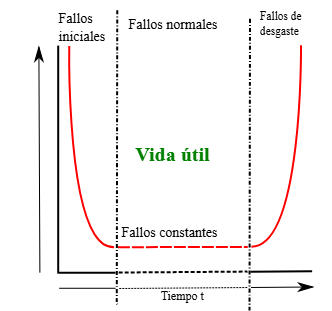
\includegraphics[scale=.7]{davies.png}
        \caption{Curva de Davies}
    \end{figure}

    \begin{enumerate}
        \item Fallos iniciales (juventud técnica):
            \begin{itemize}
                \item Alta tasa de fallas al comienzo del ciclo de vida.
                \item Causas comunes: errores de instalación, defectos de fabricación, fallas de diseño, inexperiencia del operador.
                \item En esta fase se concentran los ajustes y correcciones tempranas.
                \item Objetivo del mantenimiento: inspecciones iniciales, control de calidad, entrenamiento del personal.
            \end{itemize}
        \item Fallos aleatorios (vida util normal):
        \begin{itemize}
            \item Tasa de fallas baja y constante.
            \item Fallos producidos por causas externas e impredecibles: errores humanos, condiciones ambientales, accidentes fortuitos.
            \item Etapa ideal para aplicar el mantenimiento preventivo sistemático.
            \item Objetivo: mantener la estabilidad funcional del equipo.
        \end{itemize}
        \item Fallos de desgaste (envejecimiento):
            \begin{itemize}
                \item Aumento progresivo de la tasa de fallas debido al desgaste natural.
                \item Causas: fatiga de materiales, acumulación de ciclos de uso, deterioro físico.
                \item Objetivo del mantenimiento: anticiparse al fin de la vida útil. Se recomiendan reemplazos programados o revisiones profundas.
            \end{itemize}
    \end{enumerate}

    La clave está en identificar en qué etapa de la curva se encuentra cada equipo, y actuar en consecuencia. Un buen plan de intervenciones no se improvisa: se construye combinando datos duros (manuales, históricos) con experiencia técnica. De esa forma, el mantenimiento deja de ser reactivo y se convierte en una herramienta estratégica de confiabilidad y eficiencia operativa.

    \textbf{Ejemplo 1: Determinación del período de mantenimiento} 
    
    Determinaremos el período óptimo entre mantenimientos usando el MTBF (Tiempo Medio Entre Fallas): Es una medida de confiabilidad que indica el tiempo promedio que transcurre entre una falla y la siguiente en un equipo o componente. Se calcula como el tiempo total de operación dividido por el número de fallas.

    Se pusieron 10 elementos a funcionar durante 500 horas cada uno (tiempo total = 10 × 500 = 5,000 horas). Ocurrieron 2 fallas durante este período.

    Cálculo: MTBF = Tiempo total / Número de fallas = 5,000 horas / 2 = 2,500 horas.

    Esto significa que, en promedio, cada elemento funciona 2,500 horas antes de presentar una falla.

    \textbf{Ejemplo 2: Determinación del período de mantenimiento} 
    
    Por ejemplo, digamos que desea calcular el MTBF de un motor que funciona 8 horas al día, 5 días a la semana, durante un total de 1 año. Durante este tiempo, el motor falla 4 veces. Para calcular el MTBF
    
    Tiempo total de funcionamiento = 8 horas/día x 5 días/semana x 52 semanas = 2,080 horas
    
    Número de fallos = 4
    
    MTBF = Tiempo total de funcionamiento/ número de fallos = 2,080 horas / 4 = 520 horas
    
    El MTBF del motor es de 520 horas. Esto significa que, en promedio, se puede esperar que el motor funcione durante 520 horas antes de fallar. En realidad, podría fallar antes o después de las 520 horas y no entenderemos por qué falla el motor, pero este tiempo promedio es una métrica útil.

    \subsubsection{Mantenimiento Total Productivo (TPM)}
    El TPM (Mantenimiento Productivo Total) es una forma inteligente de cuidar las máquinas antes de que se rompan, con la ayuda de todos. No es solo tarea del técnico: los operarios también participan, haciendo tareas simples como limpiar, revisar y ajustar. La idea es no esperar a que algo falle. Porque si una máquina se rompe, se frena todo.

    Formalmente el TPM (Total Productive Maintenance) es una estrategia avanzada de mantenimiento preventivo, estrechamente vinculada al modelo Just in Time (JIT). Bajo este paradigma, la ausencia de stock de seguridad hace que cualquier falla detenga o reduzca la capacidad global del sistema productivo.

    El objetivo es lograr la máxima eficiencia de las máquinas, equipos, personas, instalaciones y sistemas, sin comprometer calidad, productividad ni tiempos de entrega. 

    Las principales pérdidas que busca eliminar son: 
    \begin{itemize}
        \item Pérdidas por averías: fallas imprevistas que detienen el proceso.
        \item Pérdidas por preparaciones o cambios de herramientas: tiempos muertos planificados mal gestionados.
        \item Paradas menores y ciclos vacíos: interrupciones breves pero repetitivas que suman grandes pérdidas.
        \item Funcionamiento a velocidad reducida: baja eficiencia del equipo.
        \item Pérdidas de calidad: productos defectuosos que requieren reprocesado o descarte.
        \item Pérdidas por puesta en marcha: ajustes y correcciones durante el arranque de un equipo.
    \end{itemize}

    La filosofia del TPM:
    \begin{itemize}
        \item Se basa en la participación activa de todos los niveles de la organización.
        \item Promueve la autonomía operativa en mantenimiento, capacitando a los operarios para realizar tareas básicas de inspección, lubricación y limpieza.
        \item Apunta a una mejora continua y sostenida del OEE (Overall Equipment Effectiveness).
    \end{itemize}

    Las características claves son:
    \begin{itemize}
        \item Participación total: involucra a todos los niveles jerárquicos, es un enfoque “top-down”.
        \item Cobertura total: abarca equipos, personas, instalaciones y procesos.
        \item Prevención total: establece un sistema preventivo que cubre toda la vida útil del equipo.
        \item Gestión por motivación: se promueven actividades autónomas en pequeños grupos, impulsadas por la dirección.
        \item Colaboración interdepartamental: une áreas de mantenimiento, operaciones e ingeniería.
    \end{itemize}

    \textbf{Los "tres totales" del TPM:} El enfoque TPM se estructura sobre tres pilares fundamentales:
    
    \begin{itemize}
        \item \textbf{Total Efectividad:} búsqueda continua de la eficiencia máxima.
        \item \textbf{Total Mantenimiento:} estrategia preventiva y predictiva a lo largo de toda la vida útil de los equipos.
        \item \textbf{Total Participación:} compromiso de todo el personal, desde operarios hasta gerentes.
    \end{itemize}

    \textbf{Las 5S japonesas:}

    \begin{figure} [ht!]
        \centering
        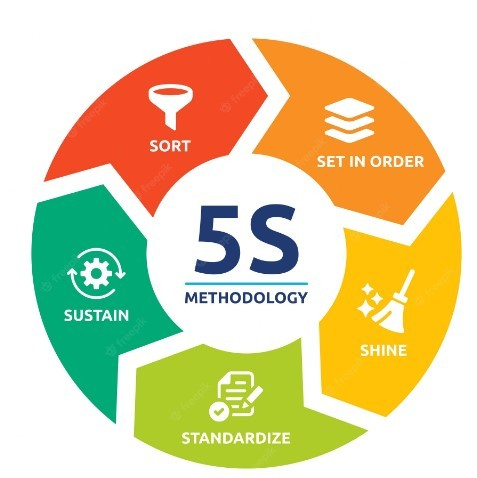
\includegraphics[width=0.5\linewidth]{5s.png}
    \end{figure}

    \begin{enumerate}
        \item Limpieza general del equipo: remoción de suciedad superficial, virutas, residuos o cualquier elemento que pueda interferir con el funcionamiento.
        \item Verificación de niveles y engrase: control y reposición de fluidos (aceite, refrigerante, hidráulico) y aplicación de lubricantes en puntos críticos.
        \item Reglajes y ajustes: revisión de topes de carrera, sensores, componentes móviles y elementos de fijación para garantizar el posicionamiento adecuado.
        \item Inspección visual y funcional básica: detección de fugas, ruidos anómalos, desgastes, holguras o condiciones inseguras.
        \item Chequeo con listas predefinidas: utilización de checklists diseñadas por el Departamento de Mantenimiento para sistematizar el control y registrar desvíos.
    \end{enumerate}


    
    \item \textbf{Mantenimiento Predictivo}

    El mantenimiento predictivo se fundamenta en la evaluación del estado operativo de una máquina en funcionamiento, con el objetivo de anticiparse a posibles fallas. Parte del principio de que los equipos emiten señales o síntomas antes de fallar, y mediante el análisis de esos síntomas, es posible predecir el momento probable de la avería.

    Características principales:
    \begin{itemize}
        \item Exige un conocimiento profundo sobre los mecanismos de degradación y fallas de los componentes.
        \item Se apoya en modelos de extrapolación confiables, que estiman el tiempo remanente de vida útil a partir de síntomas observables.
        \item Requiere establecer: frecuencia de inspección, parámetros a monitorear, instrumentos específicos de medición.
        \item Evita el submantenimiento (intervenir demasiado tarde) y el sobremantenimiento (intervenir innecesariamente).
        \item Permite optimizar la programación de tareas y organizar los recursos de forma eficiente.
    \end{itemize}

    Tipos de enfoques: 
    \begin{itemize}
        \item Si el mantenimiento se realiza al detectar un síntoma puntual, se lo denomina monitoreo en tiempo real.
        \item Si es posible analizar la evolución del síntoma y proyectar el momento de la falla, se lo considera predictivo, ya que incluye una prognosis del fallo basada en datos.
    \end{itemize}

    Ejemplos: 
    \begin{itemize}
        \item Termómetros infrarrojos que permiten medir temperaturas de tableros, bombas, motores, indicando falla.
        \item Medición de vibraciones o ruido. Permiten determinar desgaste en rodamientos, cojinetes, guías, etc.
        \item Longitud de álabes de turbina. Permite predecir creep (fluencia lenta)
    \end{itemize}

\end{enumerate}


\subsection{Gestión del Mantenimiento:}

Toda gestión eficaz del mantenimiento debe apoyarse en un plan directriz, estructurado en base al ciclo de Deming (PDCA): Planificar, Hacer, Verificar y Actuar. Esta metodología asegura la mejora continua de los procesos y permite anticiparse a fallos sistemáticamente.

La gestión debe orientarse a la eficiencia, es decir, al uso óptimo de los recursos disponibles para obtener el máximo rendimiento de los activos productivos.

Para lograrlo, se requiere un sistema de información sólido, que puede implementarse en forma manual o informática (CMMS – Computerized Maintenance Management System - Gestión de mantenimiento asistido por computadora). Este sistema permite organizar, registrar y analizar toda la información necesaria para la toma de decisiones estratégicas.

Formularios básicos que debe incluir el sistema:
\begin{itemize}
    \item Inventario o catastro de equipos: identifica todos los activos sujetos a mantenimiento.
    \item Planilla de mantenimiento preventivo: detalla las tareas a realizar por equipo.
    \item Calendario de mantenimiento: organiza las intervenciones en el tiempo.
    \item Registro de mantenimiento correctivo por máquina: permite el análisis histórico de fallas.
    \item Listado de proveedores: contacto y servicios técnicos disponibles.
    \item Listado de repuestos y repuestos por equipo: optimiza la gestión del stock.
\end{itemize}

\subsubsection{Costos de mantenimiento}

\textit{Una gestión eficaz del mantenimiento no solo debe organizar y planificar las intervenciones técnicas, sino también medir su impacto económico.
Los costos de mantenimiento constituyen una parte significativa del presupuesto industrial, y su control permite tomar decisiones informadas que optimicen la disponibilidad de los activos sin comprometer la rentabilidad de la empresa.}

\textit{Por ello, la gestión del mantenimiento debe integrar el análisis de costos como herramienta estratégica para lograr eficiencia, justificar inversiones y evitar tanto el sub como el sobre mantenimiento.}

El mantenimiento representa una porción significativa del costo total de producción, por lo tanto, impacta directamente en la rentabilidad de la empresa. Su adecuada gestión permite optimizar los recursos y reducir pérdidas por fallas, paradas no programadas o baja eficiencia operativa.

Los costos de mantenimiento se dividen en dos grandes categorías:

\begin{enumerate}
    \item \textbf{Costos fijos de mantenimiento:}

    Son independientes del volumen de producción o de las ventas.
    Incluyen aquellas acciones que se ejecutan con el fin de mantener el estado funcional de las instalaciones a mediano o largo plazo.
    Ejemplos: Salarios del personal de mantenimiento permanente, contratos de mantenimiento externo, alquiler de herramientas o infraestructura, software de gestión (CMMS), formación del personal técnico.
    \item \textbf{Costos variables de mantenimiento:}

    Están directamente relacionados con la actividad productiva: aumentan o disminuyen según el volumen de producción.
    Ejemplos: Repuestos y consumibles usados en función del desgaste por producción, energía utilizada por sistemas auxiliares (lubricación, refrigeración, etc.), horas extras por aumento de demanda, servicios de mantenimiento por eventos no programados asociados al uso intensivo.
\end{enumerate}

Los costos totales de mantenimiento resultan de la suma de los costos fijos y variables. Representan una herramienta clave para evaluar y racionalizar las decisiones dentro de la gestión del mantenimiento, ya que permiten visualizar el impacto económico real de cada estrategia aplicada.

Un análisis adecuado no debe limitarse al costo directo de intervención, sino contemplar todos los costos indirectos derivados de una falla. Por ejemplo: parada de producción, reprogramación de tarea proceso, tiempo de ocio personal.

Además, cuando se detiene una línea, se reduce el volumen de producción, lo que disminuye la absorción de los costos fijos generales de la empresa, afectando la rentabilidad global.

Por lo tanto, un enfoque profesional del mantenimiento exige integrar este análisis económico, considerando tanto el costo de intervenir como el de no intervenir.

\textbf{\textit{Impacto Económico de la Disponibilidad y la Gestión de Repuestos}}

Una alta disponibilidad de equipos reduce la necesidad de contar con máquinas de respaldo, disminuyendo la inversión y los costos financieros por capital inmovilizado.

El mantenimiento preventivo ayuda a reducir fallas y costos correctivos, pero en exceso puede disminuir la disponibilidad. Además, exige una gestión de stock de repuestos, que implica:

\begin{itemize}
    \item Costos fijos (por capital inmovilizado)
    \item Costos variables (por rotación y gestión de inventario)
\end{itemize}

\textbf{\textit{Selección de repuestos:}}

Los repuestos deben definirse no solo según manuales, sino también considerando condiciones de uso reales. Su stock puede representar entre un 5\% y 8\% del valor del equipo. La definición de niveles debe involucrar a mantenimiento, operaciones, finanzas y ventas, especialmente si hay penalidades por fallas o atrasos.


\textbf{\textit{Aspectos para fijar el nivel de stock}}

Al definir el nivel óptimo de stock se deben considerar múltiples variables técnicas y logísticas:
\begin{enumerate}
    \item Cantidad de equipos que utilizan la misma pieza.
    \item Precio del repuesto, en relación con su criticidad.
    \item Costo por rotura de stock: impacto en producción por no disponer del repuesto.
    \item Plazo de entrega total (lead time del proveedor + logística).
    \item Posibilidad de reparación de la pieza.
    \item Stock del proveedor: si es confiable y con disponibilidad inmediata, puede reducir el inventario propio.
    \item Procedencia: local o importado (impacta en plazos y riesgos).
    \item Materiales o tecnologías especiales, que pueden requerir aprovisionamiento anticipado.
\end{enumerate}

\textbf{\textit{Clasificación de repuestos:}}

\begin{itemize}
    \item Repuestos de consumo o consumibles: filtros, juntas, correas, fusibles, etc. Su consumo es alto pero el precio bajo y su plazo de entrega corto.
    \item Repuestos específicos: Son elementos propios de cada equipo. Ej.: partes
    estructurales o componentes de motor. El consumo es moderado, su precio medio y su plazo de entrega largo.
    \item Repuestos de seguridad: Son elementos imprescindibles para el funcionamiento de la fábrica. Su plazo de entrega es largo, son de alto precio y bajo consumo.
    \item Material obsoleto: elementos de equipos fuera de servicio o que no se consiguenen el mercado. Último recurso antes del remplazo del equipo.
\end{itemize}

\textbf{\textit{Tipos de contrato para tecerización (outsourcing) de Mantenimiento:}}

\begin{itemize}
    \item Contratos por administración: se establece un valor/precio por hora por especialidad y categoría. Luego se multiplica ese valor por las horas utilizadas de cada especialidad y/o categoría para determinar costo total del mantenimiento.
    \item Contrato por precio unitario - Se utiliza para volúmenes importantes y repetitivos. Se cobra por metro cuadrado, por cantidad de equipos, metros lineales (ej. Tuberías), etc. 
    \item Contrato de precio fijo: - Se pacta un valor previo a la realización del trabajo. Esto viable en trabajos que solo se realizan una vez.
\end{itemize}

\textbf{\textit{Tablero de comando:}}

Es una herramienta dinámica que muestra el desempeño organizacional en tiempo real. Permite evaluar si la gestión está alineada con los objetivos estratégicos.

Las funciones claves, son: 
\begin{itemize}
    \item Monitorea el cumplimiento de metas.
    \item Detecta desvíos en la marcha general de la organización.
    \item Redefine indicadores si los actuales no reflejan adecuadamente la misión.
    \item Identifica áreas con desempeño superior o inferior a lo esperado.
    \item Guía decisiones para mantener o corregir el rumbo de la gestión.
\end{itemize}

\textbf{\textit{Indicadores de mantenimiento:}}

Herramientas clave para evaluar la eficiencia de la gestión del mantenimiento.
Permiten tomar decisiones basadas en datos, identificar desvíos, justificar inversiones y optimizar recursos.

\begin{enumerate}
    \item Indicadores económicos
    \begin{itemize}
        \item Costo de mantenimiento por facturación:
        \begin{equation*}
            CMF = \dfrac{\text{Costo total de mantenimiento}}{\text{Facturación total}} \cdot 100
        \end{equation*}
        Mide el peso económico del mantenimiento sobre los ingresos totales. Un CMF bajo indica que el mantenimiento representa una baja proporción del negocio. Útil para análisis de rentabilidad.

        \item Costo de mantenimiento sobre producción:
        \begin{equation*}
            CMP = \dfrac{\text{Costo total de mantenimiento}}{\text{Costo total de producción}} \cdot 100
        \end{equation*}
        Mide la proporción del costo de mantenimiento respecto al costo de producción. Muestra cuánto influye el mantenimiento en el precio del producto.

        \item Índice de Preventivo sobre Total:
        \begin{equation*}
            IPP = \dfrac{\text{Costo de mantenimiento preventivo}}{\text{Costo total de mantenimiento}} \cdot 100
        \end{equation*}
        Mide el grado de enfoque preventivo del mantenimiento. Un valor elevado indica un plan preventivo bien implementado, que minimiza correctivos.
    \end{itemize}

    \item Indicadores operativos
    \begin{itemize}
        \item Índice de paradas sobre producción
        \begin{equation*}
            IPDP=\dfrac{\text{Horas de parada}}{\text{Horas de producción realizadas}} \cdot 100
        \end{equation*}
        Mide la proporción de tiempo perdido por fallas o intervenciones. Ayuda a diagnosticar la eficiencia operativa del sistema de mantenimiento.
        
        \item Índice de Utilización del Equipo Humano
        \begin{equation*}
            IUE=\dfrac{\text{Horas efectivas de mantenimiento}}{\text{Horas ddisponibles del personal}} \cdot 100
        \end{equation*}
        Mide cuánto del tiempo disponible del personal se dedica efectivamente al mantenimiento. Un IUE bajo puede reflejar demoras, tareas improductivas o mala planificación.
    \end{itemize}

    \item Indicadores de capacitación
    \begin{itemize}
        \item Índice de Capacitación del Personal de Mantenimiento
        \begin{equation*}
            ICF=\dfrac{\text{Horas de capacitación}}{\text{Horas disponibles del personal}} \cdot 100
        \end{equation*}
        Mide la inversión en formación respecto al tiempo disponible del equipo técnico. Refleja la orientación de la empresa hacia la mejora continua y el desarrollo técnico del área.
    \end{itemize}
    
\end{enumerate}

\subsection{Recursos Humanos, Higiene y Seguridad}

\textit{En el estudio del Mantenimiento Industrial, muchas veces se cree que todo gira en torno a máquinas, herramientas, repuestos y cronogramas de intervención. En realidad, ningún sistema técnico puede sostenerse sin una gestión eficaz del factor humano.}

\textit{La eficiencia del mantenimiento no solo depende de planes, indicadores y costos, sino también de las personas: su formación, motivación, seguridad y organización.}

El Recurso Humano es un factor clave en la logística y ejecución del mantenimiento. Su gestión no se limita a contratar y asignar personal, sino que debe contemplar una planificación estratégica, información precisa, desarrollo de competencias y motivación continua.

\begin{enumerate}
    \item Sistemas de información del personal

    Es fundamental disponer de un registro completo y actualizado de cada integrante del equipo de mantenimiento. Esto incluye:
    \begin{itemize}
        \item Lugar de residencia
        \item Cursos realizados
        \item Experiencia profesional
        \item Categoría laboral
        \item Legajo médico
        \item Disponibilidad y habilitaciones
    \end{itemize}
    Esta base de datos permite tomar decisiones rápidas y precisas en momentos críticos, como una parada imprevista o la asignación de tareas específicas.

    \item Planificación de recursos humanos

    Permite proyectar las necesidades de personal a corto, mediano y largo plazo.
    \begin{enumerate}
        \item \textbf{Identificación de especialidades requeridas:} Definición del perfil del puesto, es decir, las competencias técnicas y personales que debe tener quien ocupará determinado rol.

        \item \textbf{Cobertura de nuevas especialidades:} Se debe evaluar si se puede capacitar al personal existente o si será necesario incorporar nuevo personal. En caso de incorporación, se define el método: reclutamiento interno o reclutamiento externo (consultora o búsqueda directa)
    \end{enumerate}
    Esta planificación evita improvisaciones, mejora la productividad y asegura que los equipos no dependan de una sola persona.

    \item Desarrollo del Personal

    El mantenimiento moderno exige formación continua. Las tecnologías cambian, las normativas evolucionan y las exigencias aumentan. Por eso:
    \begin{itemize}
        \item La capacitación permanente es esencial.
        \item Deben priorizarse áreas que requieren habilitaciones externas, como: soldaduras especiales, ensayos no destructivos, trabajos en altura.
        \item La formación es también un elemento de motivación, promoción interna y retención del talento.
        \item Algunas tareas requieren entrenamiento práctico supervisado, más allá del conocimiento teórico.
    \end{itemize}
\end{enumerate}

Una vez que el personal ha sido correctamente planificado y capacitado, es esencial medir resultados. No basta con formar: hay que saber qué impacto tuvo esa formación y cómo se está desempeñando el equipo técnico en el día a día.

La evaluación del desempeño es una herramienta de retroalimentación para todo el sistema de mantenimiento. Permite corregir desvíos, detectar fortalezas y trazar nuevas estrategias. 

Algunos aspectos claves de la evaluación:
\begin{itemize}
    \item Nivel de conocimiento técnico: evaluación teórica y práctica.
    \item Análisis de resultados obtenidos: eficiencia, cumplimiento de tareas, solución de fallas.
    \item Plan de capacitación correctiva o complementaria, si se detectan brechas.
    \item Medición de la efectividad de las capacitaciones anteriores.
    \item Control y seguimiento de indicadores individuales y grupales.
\end{itemize}

Ahora bien, no podemos hablar de recursos humanos sin considerar el entorno en el que desarrollan sus tareas. Si no garantizamos condiciones de trabajo seguras, saludables y controladas, el mejor plan técnico y el personal más capacitado no podrán rendir al máximo.

En este contexto, la legislación juega un rol central. Veamos las dos leyes más relevantes en Argentina en materia de Higiene y Seguridad Laboral:

\begin{enumerate}
    \item Ley 19.587 – Ley de Higiene y Seguridad en el Trabajo

    Esta ley establece los principios fundamentales para proteger la vida y la integridad psicofísica del trabajador. Apunta a prevenir, reducir o eliminar los riesgos presentes en el entorno laboral.

    Los objetivos principales son: 
    \begin{itemize}
        \item Proteger la vida y salud física y mental de los trabajadores.
        \item Identificar, aislar y eliminar riesgos en los distintos sectores o puestos de trabajo.
        \item Fomentar una cultura preventiva en la organización.
        \item Estimular actitudes responsables frente a accidentes o enfermedades profesionales.
    \end{itemize}

    \item Ley 24.557 – Ley sobre Riesgos del Trabajo

    Complementa a la anterior, con una mirada más integral y moderna. Introduce el sistema de ART (Aseguradoras de Riesgo del Trabajo) y pone énfasis en la prevención, rehabilitación y compensación.

    Los objetivos principales son: 
    \begin{itemize}
        \item Reducir la siniestralidad laboral mediante acciones preventivas.
        \item Reparar daños por accidentes y enfermedades profesionales.
        \item Promover la recalificación y reinserción laboral de trabajadores afectados.
        \item Fomentar la negociación colectiva para mejorar medidas preventivas y compensatorias.
    \end{itemize}
\end{enumerate}

\textbf{\textit{Peligro vs Riesgo:}} Toda estrategia de seguridad parte de un principio básico: No se puede prevenir lo que no se entiende. Es fundamental distinguir entre dos conceptos clave en higiene y seguridad:
\begin{itemize}
    \item \textbf{PELIGRO:} Es toda fuente o agente con capacidad de causar daño. Puede tratarse de un equipo, sustancia, situación o condición. Ejemplos: un tablero eléctrico sin aislamiento, un gas tóxico, una superficie resbaladiza.
    \item \textbf{RIESGO:} Es la probabilidad de que el peligro se materialice y cause un daño efectivo.
Depende de la exposición, la frecuencia, la protección existente, etc.
\end{itemize}

\textit{Importante: No podemos protegernos de un peligro si no conocemos el riesgo que implica. Por eso, toda política de seguridad debe comenzar con la identificación y evaluación de riesgos.}

La siguiente imagen representa cuatro condiciones posibles en las que puede haber un riesgo presente y cómo la presencia o no de una persona (o su interacción con el riesgo) cambia el resultado.

\begin{figure} [ht!]
    \centering
    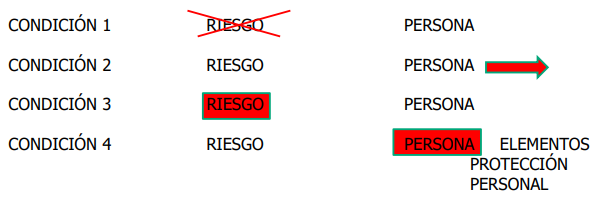
\includegraphics[scale=1]{riego persona.png}
\end{figure}

% Please add the following required packages to your document preamble:
% \usepackage{graphicx}
\begin{table}[ht!]
\resizebox{\textwidth}{!}{%
\begin{tabular}{|c|l|l|}
\hline
\textbf{Condición} & \multicolumn{1}{c|}{\textbf{Situación}}                                                                                                                 & \multicolumn{1}{c|}{\textbf{Interpretación}}                                                                                                               \\ \hline
\textbf{1}         & \begin{tabular}[c]{@{}l@{}}El riesgo está presente, pero es\\ eliminado o controlado (tachado en rojo).\end{tabular}                                    & \begin{tabular}[c]{@{}l@{}}No hay posibilidad de accidente, ya que el riesgo\\ fue neutralizado antes de que alguien esté expuesto.\end{tabular}           \\ \hline
\textbf{2}         & \begin{tabular}[c]{@{}l@{}}El riesgo está presente, pero la persona\\ no interactúa con él (flecha verde indica alejamiento).\end{tabular}              & \begin{tabular}[c]{@{}l@{}}A pesar de que hay riesgo, no hay exposición\\ directa, por lo tanto, no hay accidente.\end{tabular}                            \\ \hline
\textbf{3}         & \begin{tabular}[c]{@{}l@{}}El riesgo y la persona están en el mismo entorno\\ sin protección ni acción preventiva.\end{tabular}                         & \begin{tabular}[c]{@{}l@{}}Alta probabilidad de accidente, ya que el\\ riesgo y la persona están en contacto.\end{tabular}                                 \\ \hline
\textbf{4}         & \begin{tabular}[c]{@{}l@{}}El riesgo está presente, la persona también, pero\\ está protegida con EPP (Elemento de\\ Protección Personal).\end{tabular} & \begin{tabular}[c]{@{}l@{}}El riesgo no desaparece, pero el daño potencial\\ se mitiga. Se reduce la probabilidad o\\ gravedad del accidente.\end{tabular} \\ \hline
\end{tabular}%
}
\end{table}

La clave no es solamente eliminar el riesgo, sino gestionar la exposición. Cuando no se puede eliminar, debe protegerse al trabajador.

La siguiente imagen explica cómo influye el factor humano en la ocurrencia de accidentes, incluso cuando el riesgo está presente. Representa una especie de “cadena de defensa”.


\begin{figure} [ht!]
    \centering
    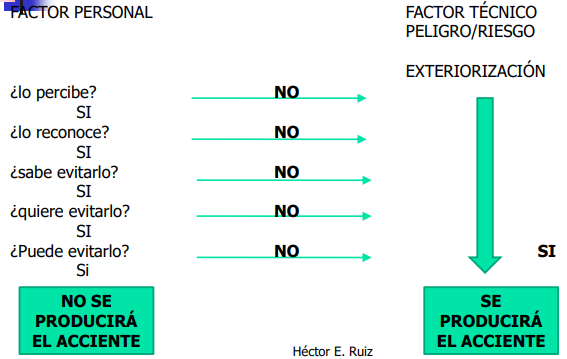
\includegraphics[width=0.6\linewidth]{factor personal.png}
\end{figure}

% Please add the following required packages to your document preamble:
% \usepackage{graphicx}
\begin{table}[ht!]
\resizebox{\textwidth}{!}{%
\begin{tabular}{|l|l|}
\hline
\multicolumn{1}{|c|}{\textbf{Pregunta}} & \multicolumn{1}{c|}{\textbf{Interpretación si la respuesta es "NO"}}   \\ \hline
¿Lo percibe?                            & Si la persona ni siquiera percibe el peligro, no puede reaccionar.     \\ \hline
¿Lo reconoce?                           & Puede verlo, pero no saber que es un peligro real.                     \\ \hline
¿Sabe evitarlo?                         & Puede reconocerlo, pero no sabe qué hacer.                             \\ \hline
¿Quiere evitarlo?                       & A veces hay negligencia o exceso de confianza.                         \\ \hline
¿Puede evitarlo?                        & Puede querer evitarlo, pero no tiene medios, formación o herramientas. \\ \hline
\end{tabular}%
}
\end{table}


Como resultado, 
\begin{itemize}
    \item Si se responde afirmativamente a todas las preguntas, NO se producirá el accidente.
    \item Si en algún punto la respuesta es “NO”, se abre paso a que el riesgo se exteriorice en un accidente real.
\end{itemize}

Como conclusión, incluso con los riesgos presentes, el factor humano es una barrera clave. Por eso la formación, concientización y empoderamiento del trabajador son tan importantes.

\textit{Ambas explicaciones se complementan. La primera imagen muestra las formas de evitar un accidente desde el entorno físico, y la segunda, desde el comportamiento humano. En conjunto nos dicen: “Controlá el riesgo, educá al operario, protegé con EPP. Si falla uno, que no fallen los demás.”}

\subsubsection{Obligaciones entre empleador y empleado}

La seguridad en el entorno laboral no es producto del azar ni de medidas aisladas. Es el resultado de un compromiso mutuo entre empleadores y empleados, alineado con la Ley 19.587 y sus disposiciones complementarias. Ambas partes tienen responsabilidades definidas que apuntan a preservar la vida, la salud y la integridad psicofísica de los trabajadores. Este enfoque integral es clave para reducir riesgos, prevenir accidentes y fomentar una cultura de trabajo segura y eficiente.

\begin{enumerate}
    \item Obligaciones del empleador:
        \begin{itemize}
          \item Realizar el examen médico preocupacional antes del ingreso laboral.
          \item Asegurar el correcto estado de conservación de máquinas y equipos.
          \item Mantener una ventilación adecuada y eliminar vapores y gases contaminantes.
          \item Verificar el correcto funcionamiento de las instalaciones eléctricas, sanitarias y de agua potable.
          \item Controlar la eliminación de residuos o acumulaciones que puedan representar un riesgo.
          \item Aislar o eliminar fuentes de ruidos y vibraciones que afecten la salud del trabajador.
          \item Proveer equipos de lucha contra incendios en condiciones operativas.
          \item Garantizar el almacenamiento seguro de sustancias peligrosas.
          \item Disponer de kits de primeros auxilios en lugares accesibles.
          \item Colocar cartelería visible que indique los riesgos y advertencias.
          \item Promover la capacitación constante del personal en temas de seguridad.
          \item Informar a la autoridad correspondiente sobre todo accidente o enfermedad laboral.
        \end{itemize}

    \item Obligaciones del empleado:
        \begin{itemize}
          \item Asistir a todas las instancias de capacitación y concientización.
          \item Cumplir estrictamente con las normas de seguridad establecidas.
          \item Utilizar de forma correcta los elementos de protección personal provistos.
          \item Comunicar cualquier accidente laboral, por leve que sea.
          \item Realizarse los estudios médicos obligatorios que disponga la empresa o la normativa vigente.
        \end{itemize}
\end{enumerate}

\clearpage

\section{Unidad 6: Planificación y Control de la Producción}

En la unidad de Mantenimiento Industrial, vimos que la anticipación y la organización de recursos son esenciales para evitar fallas, reducir costos y garantizar la disponibilidad operativa.
Aquí, en Planificación de la Producción, ese mismo enfoque se amplía a toda la empresa, buscando controlar los tiempos, recursos y actividades necesarias para cumplir con la demanda, sin improvisar ni sobrecargar el sistema.

\subsection{Planificar:}
La planificación no es un lujo, es una necesidad estratégica. En contextos industriales, donde múltiples procesos, personas y recursos interactúan, planificar permite:

\begin{itemize}
    \item Coordinar actividades internas de forma ordenada y efectiva.
    \item Anticiparse al futuro, facilitando una cultura organizacional orientada a la previsión.
    \item Controlar lo controlable, reduciendo al mínimo la incertidumbre y la improvisación.
    \item Prevenir lo indeseable, como cuellos de botella, desperdicios, sobrecostos o falta de insumos.
    \item Prepararse para lo inevitable, como mantenimientos programados o cambios en la demanda.
    \item Ser una organización controlable, en la que se pueda evaluar y ajustar decisiones.
    \item Tomar decisiones racionales, basadas en datos, experiencia y previsiones concretas.
\end{itemize}



\begin{figure} [ht!]
    \centering
    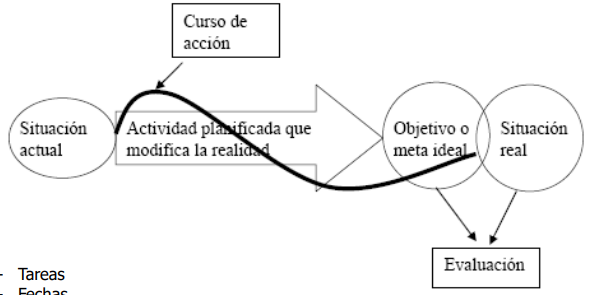
\includegraphics[scale=1]{planificar.png}
\end{figure}

La imagen anterior podemos identificar:

\begin{enumerate}
    \item \textbf{Situación actual:} Es el punto de partida, el estado real en el que se encuentra la organización, el sistema productivo, el proyecto o el entorno que queremos modificar. Ejemplo: producción desorganizada, tiempos muertos altos, entregas atrasadas.

    \item \textbf{Actividad planificada que modifica la realidad:} Este bloque simboliza la planificación en acción: tareas diseñadas estratégicamente para cambiar el estado actual. Incluye: asignación de recursos, definición de tiempos, coordinación de equipos, diseño de acciones concretas.

    \item \textbf{Curso de acción:} La línea superior representa el camino que sigue la ejecución. En la realidad, no es una línea recta: hay obstáculos, ajustes, desviaciones. Pero está guiada por un plan. \textit{"La realidad no se comporta como un Excel"}. En lugar de avanzar directo hacia el “objetivo ideal”, el curso de acción serpentea, se adapta, se ajusta. A veces avanza más rápido, a veces retrocede o toma desvíos. Pero el rumbo sigue siendo guiado por la planificación.

    \item \textbf{Objetivo o meta ideal:} Es la situación deseada, aquello que se pretende alcanzar mediante la planificación. Puede ser una mejora de productividad, reducción de costos, optimización del flujo de trabajo, etc. \textit{“Donde queremos estar.”}

    \item \textbf{Situación real (post-ejecución):} Después de ejecutar el plan, se llega a una nueva realidad. A veces se logra exactamente el objetivo… a veces no. Lo importante es que hay una transformación medible.

    \item \textbf{Evaluación:} Aquí entra el control de gestión: se compara el resultado obtenido con la meta ideal. Si hay desvíos, se identifican causas y se retroalimenta el proceso.\textit{ “¿Logramos lo que queríamos? ¿Qué ajustaríamos la próxima vez?”}
\end{enumerate}

¿Qué se gana con la planificación?

\begin{itemize}
    \item \textbf{Mejor aprovechamiento de los recursos disponibles:} La planificación formal permite utilizar de forma eficiente los activos, evitando desperdicios y tiempos muertos.
    \item \textbf{Identificación de causas cuando no se alcanzan los objetivos:} Cuando la planificación está bien formulada y no se logra el objetivo, es posible detectar con claridad si el fallo se debió a factores externos (económicos, políticos, logísticos, etc.).
    \item \textbf{Promueve la reflexión estratégica:} Obliga a pensar de forma estructurada sobre hacia dónde se quiere ir y cómo se va a llegar, generando alineación entre los equipos.
    \item \textbf{Anticipación al cambio:} La planificación no elimina los cambios, pero permite preverlos y diseñar respuestas eficaces, transformando incertidumbre en previsibilidad.
    \item \textbf{No reduce la flexibilidad, la organiza:} La planificación no implica rigidez: si algo cambia, se replanifica. Lo importante es que existe una base racional desde la cual ajustar el rumbo.
\end{itemize}

\subsection{Enfoque jerárquico para el proceso de planificación y control de la producción}

\begin{figure} [ht!]
    \centering
    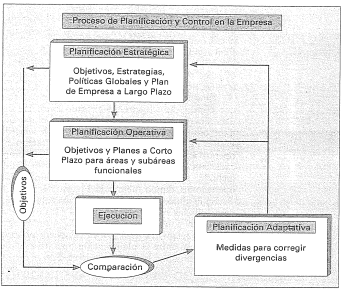
\includegraphics[scale=1]{niveles.png}
\end{figure}

En el ámbito empresarial, la planificación se estructura en diferentes niveles jerárquicos, cada uno con objetivos, horizontes temporales y grados de detalle distintos. A continuación, se describe cada uno de estos niveles aplicados a una empresa de alimentos ficticia, llamada AlimDelicias S.A., dedicada a la producción y comercialización de galletitas, cereales y snacks.

\begin{enumerate}
    \item \textbf{Planificación Estratégica}

    Es la planificación de más alto nivel. Se encarga de definir los grandes objetivos de la empresa y las estrategias necesarias para alcanzarlos. Este nivel está orientado al largo plazo (generalmente entre 3 y 5 años) y es responsabilidad de la Alta Dirección.

    \textit{Ejemplo: La empresa decide lanzar una nueva línea de productos saludables para ampliar su participación en el mercado. También planea instalar una nueva planta productiva en otra provincia para acercarse a nuevos centros de consumo.}

    \item \textbf{Planificación Táctica}

    Este nivel conecta la estrategia con la operación. Aquí se transforman los objetivos estratégicos en planes más concretos para cada área funcional (producción, recursos humanos, marketing, logística, etc.). Se trabaja en un horizonte de mediano plazo, que puede ir de varios meses hasta dos años.

    \textit{Ejemplo: El gerente de producción elabora un plan agregado que estima producir 90.000 kg mensuales de cereales, distribuidos en tres sabores. El departamento de RRHH diseña un plan de contratación de 25 nuevos operarios para la nueva planta. A su vez, marketing programa campañas de lanzamiento para el nuevo producto.}

    \item \textbf{Planificación Operativa}

    En este nivel se bajan los planes tácticos al día a día de la producción. La planificación operativa define qué se va a hacer, cuándo, dónde y con qué recursos. Se maneja información altamente detallada y se actúa sobre un horizonte corto: semanas, días o incluso turnos de trabajo.

    \textit{Ejemplo: Se programa que el lunes se producirá el cereal con miel, el martes el de frutas, y el miércoles el de chocolate. Se genera un plan de materiales que indica cuánta avena, azúcar, envases y aditivos serán necesarios para cumplir con el programa de producción. Además, se asignan los turnos de trabajo y las máquinas que se utilizarán.}

\end{enumerate}
Planificación Adaptativa:

Este tipo de planificación no responde a un nivel jerárquico fijo, sino que atraviesa a todos los anteriores. Su objetivo es monitorear lo que realmente sucede y realizar los ajustes necesarios en caso de desviaciones respecto de los planes establecidos.

\textit{Ejemplo: Si se detecta una caída inesperada en las ventas de un producto, el área de producción ajusta su programa reduciendo la fabricación. Si una máquina clave se detiene por una falla, se reorganiza el turno y se cambia el orden de producción para evitar retrasos.}
Cada nivel de planificación está conectado con el siguiente. La estrategia marca el rumbo general, la táctica traduce ese rumbo en planes concretos por área, la operativa ejecuta con precisión en el corto plazo, y la planificación adaptativa se asegura de que todo el sistema mantenga el rumbo correcto ante los cambios del entorno.


\begin{figure} [ht!]
    \centering
    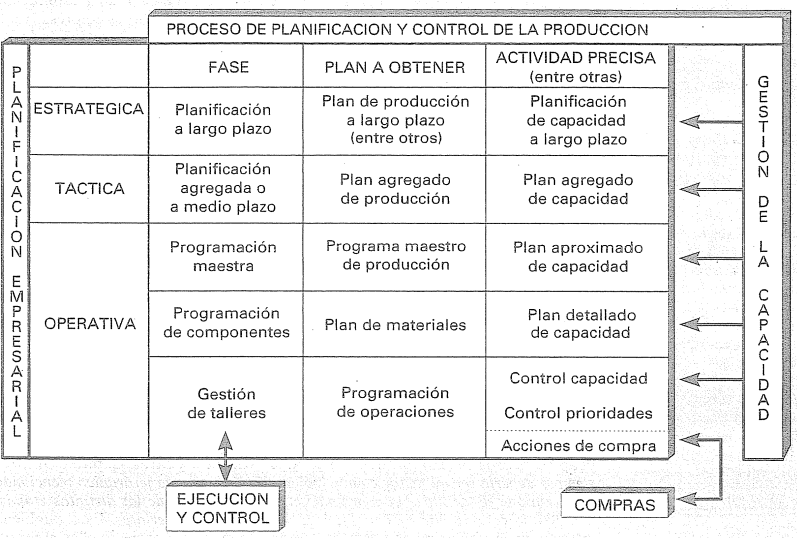
\includegraphics[scale=0.7]{jerarquia.png}
\end{figure}


Las organizaciones / empresas se organizan las decisiones de producción según plazo temporal, responsabilidad jerárquica y foco de acción.

\begin{table}[ht!]
\centering
\begin{tabular}{|l|l|l|}
\hline
\multicolumn{1}{|c|}{\textbf{Nivel}}                                                              & \multicolumn{1}{c|}{\textbf{Responsables}}                           & \multicolumn{1}{c|}{\textbf{En qué consiste}}                                                                                                                                                                                                                                                                                                                                                     \\ \hline
\textbf{\begin{tabular}[c]{@{}l@{}}Nivel Estratégico\\ (Objetivos a largo \\ plazo)\end{tabular}} & \textbf{Directores}                                                  & \begin{tabular}[c]{@{}l@{}}Se toman decisiones que impactan en el largo \\ plazo (varios años). Incluye:\\ • Definir la capacidad de producción.\\ • Elegir la ubicación y el tipo de proceso.\\ • Elaborar el plan de producción y ventas a largo\\ plazo.\\ • Hacer el dimensionamiento de la instalación.\\ \\ Definen los recursos.\end{tabular}                                              \\ \hline
\textbf{Nivel Táctico}                                                                            & \textbf{\begin{tabular}[c]{@{}l@{}}Gerentes\\  o Jefes\end{tabular}} & \begin{tabular}[c]{@{}l@{}}Se gestiona el mediano plazo (6 a 18 meses). \\ No se modifica la capacidad instalada,\\ pero se ajusta la operación.\\ Incluye:\\ • Hacer el Plan Agregado de Producción.\\ • Equilibrar la demanda con la capacidad.\\ • Considerar inventarios, materias primas y\\ capacidad externa.\\ • Asignar mano de obra disponible.\\ \\ Administran recursos.\end{tabular} \\ \hline
\textbf{Nivel Operativo}                                                                          & \textbf{Supervisores}                                                & \begin{tabular}[c]{@{}l@{}}Corresponde al corto plazo (semanas o meses).\\ Se bajan los planes a acciones concretas.\\ Incluye:\\ • Desarrollar el Programa Maestro de Producción.\\ • Coordinar entregas y actividades diarias.\\ \\ Aquí se hace la programación del trabajo.\end{tabular}                                                                                                      \\ \hline
\end{tabular}
\end{table}

\clearpage

\subsection{Plan Agregado de producción}

\begin{figure} [ht!]
    \centering
    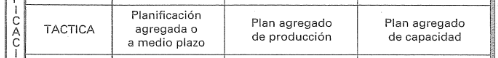
\includegraphics[scale=.8]{tctica.png}
\end{figure}

En el contexto de la gestión TÁCTICA, la planificación agregada representa un eslabón fundamental entre las decisiones estratégicas de largo plazo y la ejecución operativa. Se trata de una herramienta de planificación táctica que permite determinar cuánto producir, con qué recursos y en qué períodos de tiempo, de forma tal que se logre satisfacer la demanda proyectada con la máxima eficiencia posible.

Su importancia radica en la capacidad de equilibrar la oferta con la demanda dentro de un horizonte de mediano plazo (habitualmente de 3 a 18 meses), tomando en cuenta limitaciones reales como la capacidad instalada, la disponibilidad de personal y los costos asociados. A través de esta planificación, las organizaciones pueden evitar tanto la sobreproducción como los faltantes, alineando los objetivos de rentabilidad, eficiencia y servicio al cliente.

La planificación agregada no opera en el vacío: coordina y traduce las decisiones estratégicas en acciones operativas concretas, siendo un elemento esencial para la coherencia y sostenibilidad del sistema productivo. En definitiva, permite transformar la estrategia en acción, asegurando que los recursos se utilicen de manera óptima sin comprometer los objetivos a largo plazo.

\textit{¿Qué se busca con la Planificación Agregada?}

\begin{itemize}
    \item Cumplir con el Plan Estratégico de la empresa.
    \item Equilibrar oferta y demanda en el mediano plazo.
    \item Minimizar costos (mano de obra, inventario, planta y equipo, subcontratación), sin descuidar la satisfacción de la demanda.
    \item No comprometer los objetivos estratégicos por decisiones tácticas.
    
\end{itemize}

La Planificación Agregada determina el volumen de producción y los recursos necesarios (como personal, turnos, materiales e inventario) para responder a la demanda prevista en un horizonte de tiempo determinado (usualmente de 3 a 18 meses).

¿Por qué es tan importante?
\begin{itemize}
    \item Coordina los objetivos del nivel estratégico (más general) con las decisiones del nivel operativo (más específico).
    \item Parte de la base de que la capacidad instalada ya fue definida en el nivel estratégico.
    \item Manejar variables clave como: niveles de producción, inventarios, horas de trabajo y personal, subcontrataciones o turnos extras.
\end{itemize}

Se presentan tres gráficos/casos que muestran diferentes estrategias de planificación agregada, comparando dos curvas acumuladas a lo largo del tiempo:
\begin{itemize}
    \item \textbf{Capacidad acumulada (línea punteada gruesa):} es lo que la empresa puede producir.
    \item \textbf{Demanda acumulada (línea fina):} es lo que el mercado requiere.
\end{itemize}

La relación entre las pendientes y sus diferencias nos ayuda a visualizar si hay exceso de capacidad (sobreproducción) o déficit (falta de producción), y con eso evaluar decisiones como acumulación de inventarios, horas extras o tercerización.

El primer caso presenta capacidad constante, demanda creciente al final. La pendiente de la capacidad es constante (producción estable). La demanda crece más lentamente al principio y se acelera después. Esto implica: generar stock sobrante al inicio (capacidad > demanda). Luego hay déficit de capacidad (demanda > capacidad). Se opta por una \textbf{producción regular} (estrategia de nivelación) y se usa el inventario como colchón.
\begin{figure} [ht!]
    \centering
    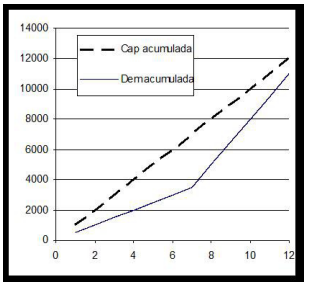
\includegraphics[scale=.7]{1.png}
\end{figure}

En el segundo caso, la demanda acumulada crece más rápido al inicio que la capacidad. Esto lleva: requerir producción adicional desde el inicio y posible uso de horas extras, contratación temporal o subcontratación. Se opta por una \textbf{estrategia de seguimiento de demanda} (se ajusta la producción para no perder ventas).
\begin{figure} [ht!]
    \centering
    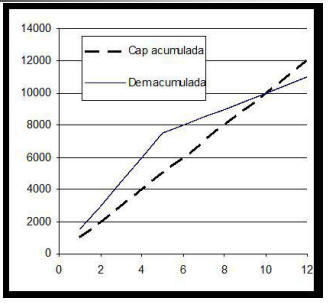
\includegraphics[scale=0.7]{2.png}
\end{figure}

El tercer caso representa una coincidencia casi perfecta. Las pendientes de ambas curvas coinciden casi por completo. Esto implica: que no hay invntarios ni faltantes significativos. Se logra un equilibrio óptimo entre capacidad y demanda. Es un caso ideal. Generalmente requiere una planificación muy fina o ajustes dinámicos.
\begin{figure} [ht!]
    \centering
    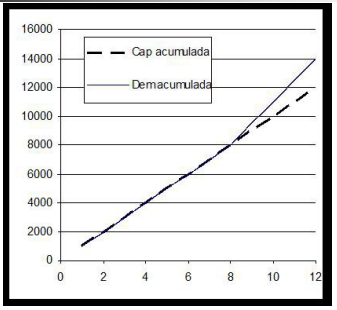
\includegraphics[scale=0.7]{3.png}
\end{figure}

A continuación, se presentan las herramientas que se utilizan dentro de la planificación agregada para alcanzar ese equilibrio entre capacidad y demanda que venimos analizando.

Para satisfacer la demanda prevista de la manera más eficiente, sin perder de vista los costos ni los objetivos estratégicos, se ajustan variables que sí se pueden manejar en el corto y mediano plazo:

\begin{enumerate}
    \item \textbf{Ritmo de la producción:} aumentas o reducir la producción mensual o semanal. Implica ajustes en turnos, uso de maquinaria, o incorporación de horas extra.

    \item \textbf{Fuerza de Trabajo (Mano de Obra):} aumentar o disminuir personal fijo o temporal. Se puede contratar, despedir, capacitar, o reubicar trabajadores según la carga de trabajo.

    \item \textbf{Nivel de Inventario:} se puede acumular stock cuando la demanda es baja para cubrir picos futuros. También se puede usar el inventario existente para evitar sobredimensionar la producción.
\end{enumerate}

Las mencionadas anteriormente son las clásicas. Además, podemos mencionar: subcontratación (outsourcing), backordering (pedidos pendientes o entrega diferida), precios o promociones para manejar demanda, horas extra o turnos adicionales.

Una vez definidos los objetivos de la planificación agregada, las variables que se pueden ajustar, el siguiente paso es elegir la estrategia más adecuada para responder a la demanda prevista. Existen distintas formas de abordar este desafío, y cada una representa un equilibrio distinto entre costos, flexibilidad y capacidad de respuesta.

\begin{enumerate}
    \item \textbf{Estrategia de alcance}

    Consiste en ajustar la producción al ritmo de la demanda, variando la cantidad de mano de obra, turnos o equipos necesarios en cada período. Se busca igualar 
    producción con demanda mes a mes.

    Entre las principales ventajas se destaca la minimización de inventarios, ya que se produce lo justo para cubrir la demanda sin acumular stock. Además, si se aplica correctamente, permite evitar faltantes de productos.

    Sin embargo, esta estrategia también presenta desventajas importantes, como los costos asociados a contrataciones y despidos frecuentes, la inestabilidad laboral y los posibles efectos negativos sobre la moral del personal. También puede generar dificultades operativas si las variaciones de demanda son muy abruptas o impredecibles.

    \textit{Ejemplo práctico:
    Una fábrica de heladeras aumenta personal en verano para responder a la mayor demanda, y reduce en invierno. La producción “sigue” a la demanda, incluso contratando temporarios.}

    \item \textbf{Estrategia de nivelación}

    En esta estrategia, la empresa mantiene un nivel de producción uniforme a lo largo del tiempo, independientemente de las fluctuaciones en la demanda. Esto implica sostener una fuerza de trabajo constante, evitando contrataciones o despidos según los vaivenes del mercado. El objetivo es minimizar los costos asociados a los cambios de personal y optimizar la eficiencia operativa, utilizando los recursos de forma estable y predecible.

    Cuando la demanda supera la capacidad de producción, se recurre a inventarios acumulados previamente, y cuando la demanda es menor, se almacena el excedente producido. También pueden utilizarse mecanismos adicionales, como promociones, descuentos o ventas fuera de temporada, para redistribuir la demanda y alinearla con la capacidad disponible.
    
    Esta estrategia reduce los costos de producción y estabiliza las operaciones, pero requiere una \colorbox{BurntOrange}{buena planificación de inventarios y una infraestructura adecuada para almacenamiento}. 
    
    Además, puede resultar riesgosa si la demanda es altamente volátil o impredecible, ya que se corre el \colorbox{BurntOrange}{riesgo de generar sobrestocks o quiebres de inventario}. 

\textit{Ejemplo práctico:
    Una fábrica de heladeras produce 10.000 unidades por mes todo el año, aunque la demanda es mayor en verano. Durante los meses de baja demanda acumula inventario, y en los de alta, vende el stock acumulado. Así, mantiene estable su fuerza laboral y minimiza los costos de producción, aunque asume costos de almacenamiento.}
\end{enumerate}

\begin{figure} [ht!]
    \centering
    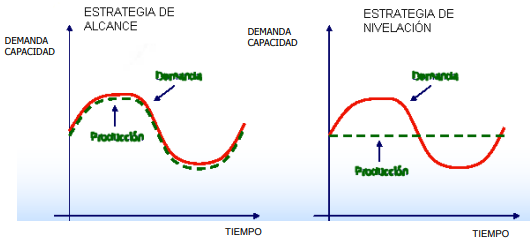
\includegraphics[scale=.9]{estrategias.png}
\end{figure}

\subsubsection{Ejemplo de estrategia de alcance}

\begin{figure} [ht!]
    \centering
    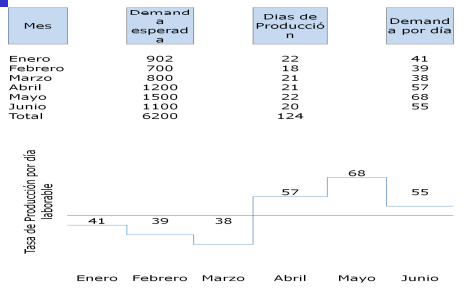
\includegraphics[scale=1]{ejemlo alcance.png}
\end{figure}

\subsubsection{Problema}

Realizar una plan agregado de producción una empresa que presta servicios de atención
telefónica, con un tiempo de 15 minutos estándar para la atención de cada cliente.
 a) Explicar brevemente que tipo de estrategia se deberá seguir
 b) Completar el siguiente plan agregado

\begin{figure} [ht!]
    \centering
    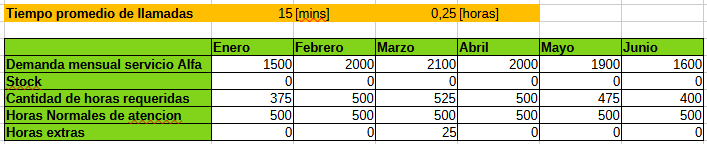
\includegraphics[scale=.9]{tablita.png}
\end{figure}

Utilizo la estrategia alcance. Por más que haya una cierta cantidad de horas fijas, al ser un servicio, los operarios se 'amoldan' a la cantidad de llamadas presentes en los distintos momentos de la jornada. Además, si fuese el caso, como en marzo, tendrían que realizar horas extras para satisfacer la cantidad de llamadas.

\subsubsection{Unidad de medida agregada}

Una unidad de medida agregada representa un conjunto de productos o servicios que comparten los mismos recursos clave para su producción o prestación. Permite planificar en términos globales sin entrar en el detalle individual de cada producto.

Se utiliza ya que simplifica la planificación agregada, permite estimar la demanda y los recursos requeridos con mayor eficiencia, reduce la complejidad en entornos con múltiples productos similares.

\textbf{Por ejemplo:} Automóviles sedán, hatchback y SUV de una misma línea de montaje. Comparten: mano de obra especializada, estaciones de soldadura, pintura y montaje, componentes comunes como neumáticos, asientos, sistemas eléctricos

\subsubsection{Horizonte de planificación}

Es el período de tiempo que cubre el plan de producción o prestación de servicios.
Ejemplos: Trimestral, semestral o anual.
La elección depende del tipo de industria y la estabilidad de la demanda.

\subsubsection{Cubos de tiempo}

Son los intervalos temporales en los que se divide el horizonte. Pueden ser semanas o meses. Al finalizar cada cubo, se revisa el desempeño real y se ajusta el plan si es necesario. Aquí se introduce el concepto de "control" en el ciclo de planificación y control de la producción.

\subsubsection{Etapas de la planificación agregada}

\begin{enumerate}
    \item \textbf{Previsión de la demanda:} Se estima la demanda futura para cada producto individualmente. Esto puede basarse en datos históricos, estacionalidad o tendencias de mercado.
    \item \textbf{Demanda agregada global:} Se transforma la demanda específica en una demanda total expresada en unidades agregadas, para simplificar el análisis y facilitar la toma de decisiones.
    \item \textbf{Cálculo de recursos necesarios:} A partir de la demanda agregada, se determinan los recursos que se necesitarán: horas hombre, horas máquina, materias primas, etc.
    \item \textbf{Identificación de estrategias alternativas:} Se exploran distintos enfoques posibles para satisfacer la demanda. Ejemplos: ajustar inventarios, contratar personal temporal, subcontratar producción, etc.
    \item \textbf{Selección de estrategia óptima:} Se elige la alternativa que mejor cumpla con los objetivos organizacionales, minimizando costos y manteniendo el servicio o producción requeridos.
\end{enumerate}

\subsubsection{Factores que afectan la Planificación Agregada}

\begin{itemize}
    \item Factores internos: Son elementos que dependen directamente de la organización. Determinan su capacidad productiva actual.
    \begin{itemize}
        \item Capacidad física actual: maquinaria, espacio, infraestructura disponible.
        \item Fuerza laboral actual: cantidad, especialización y disponibilidad del personal.
        \item Niveles de inventario: stock de productos terminados, en proceso o materias primas.
        \item Actividades requeridas para la producción: procesos, tiempos estándar, complejidad operativa.
    \end{itemize}
    \item Factores externos: Son variables del entorno que afectan las decisiones pero están fuera del control directo de la empresa.
    \begin{itemize}
        \item Disponibilidad de materias primas: acceso, tiempos de entrega, calidad.
        \item Comportamiento de competidores: estrategias comerciales o productivas que puedan alterar la demanda.
        \item Capacidad externa subcontratable: posibilidad real de tercerizar producción o servicios.
        \item Demanda del mercado: nivel, estacionalidad, variabilidad.
        \item Condiciones económicas: inflación, tipo de cambio, legislación laboral, etc.
    \end{itemize}
\end{itemize}

\subsubsection{Variables de ajustes}

Durante la planificación, la empresa cuenta con "palancas de control" para adaptar la oferta o influenciar la demanda, dentro de sus posibilidades.

\begin{itemize}
    \item Variables que modifican la oferta:
    \begin{itemize}
        \item Contratación / despido de personal: modificar la fuerza laboral para adaptarse a la demanda.
        \item Trabajo en tiempo extra: aumentar producción sin incorporar personal.
        \item Personal eventual / suspensiones: dar flexibilidad al esquema de trabajo.
        \item Nivel de inventarios (solo en bienes físicos): producir para stock o consumir stock acumulado.
        \item Outsourcing / subcontratación: derivar parte de la producción a terceros.
        \item Ajustes estructurales: inversiones o cambios en la planta que amplían capacidad.
    \end{itemize}
    
    \item Variables que influyen en la demanda:
    \begin{itemize}
        \item Cambio de precios: incentiva o frena el consumo.
        \item Aumento de vendedores: fuerza comercial más agresiva.
        \item Promociones y publicidad: campañas para estimular ventas.
        \item Productos complementarios: vender productos que arrastren el consumo del producto principal.
    \end{itemize}
\end{itemize}

 %ESTA FOTO NO VA ACAAA!!!


\subsubsection{Indicadores Clave de Rendimiento Operativo}
\begin{itemize}
    \item Factor de Utilización (U): mide el grado de uso efectivo de la capacidad disponible. Indica qué porcentaje del tiempo total disponible realmente se utilizó para producir. Valor entre 0 y 1 (o expresado en \%). Un valor de 0,85 significa que se utilizó el 85% del tiempo disponible en actividades productivas

    \begin{equation*}
        U = \dfrac{\text{Horas Productivas Utilizadas}}{\text{Horas reales disponibles}}
    \end{equation*}

    \item Factor de Eficiencia (E): mide qué tan eficiente fue el uso del tiempo productivo. Las horas estándar son el tiempo teórico ideal para producir cierta cantidad; este indicador refleja la diferencia entre lo que debería haber tardado y lo que realmente tardó. 
    \begin{equation*}
        E = \dfrac{\text{Horas estandar}}{\text{Horas productivas utilizadas}}
    \end{equation*}
    \begin{itemize}
        \item Si E = 1 → producción exactamente en el tiempo estimado.
        \item Si E > 1 → mayor eficiencia (se produjo más rápido que lo previsto).
        \item Si E < 1 → menor eficiencia (se tardó más de lo previsto).
    \end{itemize}
\end{itemize}

\subsection{El Plan Maestro de Producciópn (PMP)}
\begin{figure} [ht!]
    \centering
    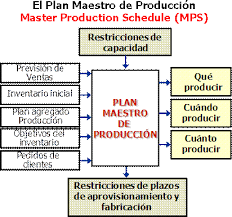
\includegraphics[scale=0.8]{pmpcuadrooo.png}
\end{figure}
El PMP traduce el Plan Agregado en un cronograma concreto de fabricación de productos terminados, especificando qué se va a producir, cuánto y cuándo. Se focaliza en ítems individuales con fechas y cantidades definidas.

El objetivo del PMP, es:
\begin{itemize}
    \item Operativizar el Plan Agregado, desagregando productos o servicios.
    \item Evaluar viabilidad frente a capacidad instalada y disponibilidad de recursos.
    \item Incorporar pedidos reales al cronograma de producción.
    \item Optimizar el uso de recursos, evitando cuellos de botella o tiempos muertos.
    \item Coordinar con Finanzas, proyectando necesidades de flujo de fondos.
    \item Sincronizar con Ventas, alineando producción con entregas programadas.
\end{itemize}

La naturaleza del PMP:
\begin{itemize}
    \item Dinámico: requiere revisión periódica frente a cambios de demanda, disponibilidad o imprevistos.
    \item Flexible: permite ajustes sin desestabilizar el sistema productivo.
\end{itemize}

\begin{figure} [ht!]
    \centering
    \includegraphics[width=0.5\linewidth]{pmpcuadro.png}
\end{figure}


\begin{figure} [ht!]
    \centering
    \includegraphics[width=0.75\linewidth]{pmpej.png}
\end{figure}



\clearpage
\subsubsection{Programación de Componentes (MRP)}

El MRP es el sistema que permite traducir el PMP (demanda independiente) en necesidades detalladas de componentes y materias primas (demanda dependiente), respondiendo a la pregunta: ¿Qué materiales necesito? ¿Cuándo y en qué cantidad?

Relación con el PMP: 
\begin{itemize}
    \item Entrada: Plan Maestro de Producción (PMP), niveles actuales de inventario, pedidos de materiales en curso.
    \item Salida: plan detallado de pedidos de materiales (que comprar, cuanto y cuando)
\end{itemize}

Elementos estructurales (datos fijos):
\begin{itemize}
    \item BOM (Bill of Materials – Lista de materiales): descompone cada producto final en sus componentes.
    \item Hoja de Ruta: secuencia de operaciones necesarias para fabricar cada ítem (procesos, máquinas, tiempos, centros de trabajo).
\end{itemize}


Este esquema básico de MRP permite:

Anticiparse a las necesidades reales de componentes.
Evitar faltantes o excesos de inventario.
Sincronizar compras y producción.

\begin{figure} [ht!]
    \centering  \includegraphics[width=0.75\linewidth]{mrp ejemplo.png}
\end{figure}
\clearpage

\section{Capítulo 7: Dirección de operaciones}

La Dirección de Operaciones es el área encargada de planificar, organizar y supervisar los procesos productivos de una empresa. Su función central es transformar insumos (materiales, trabajo, tecnología, información) en bienes y servicios que satisfagan las necesidades del cliente, de forma eficiente, eficaz y rentable.

En otras palabras, es la disciplina que garantiza que lo prometido por Marketing y financiado por Finanzas se concrete en productos o servicios reales, entregados a tiempo, con calidad y al costo adecuado.

Es una función estratégica que impacta directamente en la competitividad. Desde una industria automotriz hasta una cadena de comida rápida, la Dirección de Operaciones define cómo se produce, con qué recursos y bajo qué condiciones.

En síntesis: es el cerebro y la columna vertebral de la producción. Sin ella, no hay entrega ni experiencia de cliente.

Toda empresa, desde una multinacional hasta una pyme local, se apoya en tres pilares clave:

\begin{itemize}
    \item Marketing / Ventas: Genera la demanda. Identifica necesidades, posiciona productos y cierra ventas. Ej.: Una cervecera lanza una campaña para su nueva IPA.

    \item Finanzas: Asegura el flujo de dinero necesario para operar. Administra inversiones, costos y riesgos. Ej.: Una startup busca financiamiento para escalar su producción de drones.

    \item Operaciones: Convierte insumos en bienes o servicios. Produce lo que la empresa vende. Ej.: Una fábrica de colchones transforma espuma, resortes y telas en unidades listas para despacho.
\end{itemize}


La Administración de Operaciones (OM) se ocupa de diseñar, planificar, controlar y mejorar los procesos que permiten transformar recursos en valor.

Es decir, es el corazón productivo de la empresa: si Marketing promete y Finanzas financia, Operaciones cumple.

Ej.: En un hospital, operaciones organiza desde el quirófano hasta la limpieza. En un taller mecánico, desde la recepción del vehículo hasta la entrega del auto reparado.

\textbf{Función:}

Es la encargada de entregar el producto o servicio que el cliente espera. Puede:
\begin{itemize}
    \item Producir bienes físicos (una bicicleta, un par de zapatillas)
    \item Brindar servicios (una consulta médica, un curso online)
    \item O una combinación (una aerolínea ofrece el vuelo –servicio– y comida –bien físico–)
\end{itemize}

\textit{Ej.: Netflix entrega contenido digital (servicio), pero también opera centros de datos (bienes tangibles).}

\textbf{¿Por qué estudiar Administración de Operaciones?}

\begin{enumerate}
    \item Es una de las tres funciones clave de cualquier empresa. (Vender, financiar y producir)
    \item Te enseña cómo se genera lo que el cliente recibe, desde una pizza hasta un avión.
    \item Permite entender qué decisiones toma un Director de Operaciones y cómo optimiza recursos.
    \item Impacta directamente en los costos e ingresos: una mala operación mata la rentabilidad; una buena, te lleva a jugar en primera.
\end{enumerate}
\textit{Ej.: Amazon optimiza sus centros de distribución al extremo. Esa eficiencia operativa es su ventaja competitiva.}


\textbf{Ejemplo}

Este cuadro es una comparación entre las tres funciones clave de una empresa (Marketing, Finanzas y Operaciones) y su impacto en la contribución económica final de la organización. Se usa para mostrar cómo cada área puede mejorar los resultados, pero también para destacar que la Dirección de Operaciones tiene un rol fundamental en la rentabilidad.

\begin{figure} [ht!]
    \centering
    \includegraphics[scale=.6]{cuadro_do.png}
\end{figure}

En actual, representamos la situación base de la empresa. Sirve como punto de partida para comparar. Luego tenemos 3 opciones: a) marketing: supone un aumento del 50\% de las ventas. b) Supone el 50 \% de la reduccion de costos financieros (desembolsos que debe hacer la empresa cuando obtiene financiamiento a través de deudas, como crédito bancario, financiamiento gubernamental, fondos de capital de riesgo, socios con capital o business angels, entre otros.) y por ultimo la opcion c) Supone una reducción del 20\% en el costo de producción.

Como conclusión del cuadro, aunque las tres áreas mejoran la rentabilidad, la mejora más significativa proviene de Dirección de Operaciones. Esto demuestra cómo optimizar procesos productivos puede tener un mayor impacto financiero que solo vender más o reducir intereses.


\textit{Ejemplo real: En una fábrica de autopartes, reducir el desperdicio o mejorar el layout puede generar ahorros muy superiores a una campaña de marketing o una negociación con el banco.}


\begin{figure} [ht!]
    \centering
    \includegraphics[width=0.75\linewidth]{pasado-futuro.png}
\end{figure}

El cuadro resume cómo ha cambiado la gestión de operaciones a lo largo del tiempo, en función de las causas impulsoras. Muestra el contraste entre cómo se hacían las cosas antes y hacia dónde se dirigen las empresas modernas.

\begin{itemize}
    \item Enfoque nacional o local → Enfoque global: Antes las empresas operaban dentro de fronteras. Hoy, gracias a las redes de comunicación y transporte baratas y confiables, el comercio es global.
    \item Envío de remesas grandes → Envíos “justo a tiempo”: Antes se almacenaban grandes lotes por seguridad. Hoy se busca minimizar inventarios usando sistemas como JIT (Just In Time), que reducen costos y aumentan eficiencia.
    \item Adquisición de la mejor oferta → Alianzas estratégicas: Ya no basta con buscar el precio más bajo. Hoy se valora a los proveedores que mejoren la calidad del producto, colaborando como socios estratégicos.
    \item Lento desarrollo del producto → Desarrollo ágil: Ciclos de vida más cortos, internet y software de diseño permiten una innovación más rápida. Ej: Tesla actualiza sus autos vía software, sin rediseñar el hardware.
    \item Productos estandarizados → Personalización en masa: Antes se fabricaba en serie sin diferenciación. Hoy se buscan productos personalizados que aún se fabriquen con eficiencia. Ej: zapatillas Nike a medida.
    \item Especialización de trabajos → Equipos autogestionados: Antes se dividían tareas al extremo. Hoy se buscan equipos multifuncionales, empoderados para tomar decisiones y adaptarse. Ej: células de trabajo en Toyota.
\end{itemize}

\subsection{SISTEMAS}
    
    Un sistema es un conjunto organizado de elementos que están interrelacionados y trabajan en conjunto para lograr un objetivo común. Estos elementos pueden ser físicos (máquinas, personas), conceptuales (ideas, normas) o una mezcla de ambos, y están delimitados por fronteras que los separan del entorno.
    
    Las características clave de un sistema:
    \begin{itemize}
        \item Tiene un objetivo definido: Todo sistema busca cumplir una función específica.
        \item Está compuesto por partes: Cada parte cumple un rol, pero ninguna tiene sentido por sí sola sin el contexto del conjunto.
        \item Existe interdependencia: Los cambios en una parte afectan al resto.
        \item Genera sinergia: El resultado del sistema es mayor que la suma de sus partes.
        \item Interactúa con el entorno: A través de entradas (inputs) y salidas (outputs).
        \item Puede ser abierto o cerrado: Dependiendo de si intercambia información, energía o materia con el exterior.
    \end{itemize}
    
    En resumen, un sistema no es simplemente una colección de cosas, sino una organización de partes con propósito y relaciones estructuradas que hacen que funcione como un todo coherente.
    
    Además, los sistemas presentan una serie de características fundamentales que permiten entender su comportamiento y estructura:
    
    \begin{itemize}
        \item \textbf{Objetivo:}
    
        Todo sistema existe por una razón: tiene un propósito definido. Sus elementos trabajan de forma coordinada para cumplir esa función principal. Por ejemplo, el objetivo de un sistema de producción es transformar insumos en productos terminados.
        
        \item \textbf{Globalidad:}
    
        En un sistema, \colorbox{BurntOrange}{ninguna parte actúa de forma completamente aislada.} Un estímulo que afecta a un componente puede repercutir en todo el sistema. Esto implica que cualquier cambio, aunque parezca localizado, puede generar efectos en cadena. Es el principio de la interdependencia sistémica.
        
        \item \textbf{Homeostasis:}
    
        Los sistemas tienden a mantener un equilibrio dinámico frente a los cambios. Esta capacidad de autorregulación les permite adaptarse tanto a alteraciones internas como externas, para seguir funcionando adecuadamente. Un ejemplo biológico es la temperatura corporal, que se ajusta constantemente a pesar de las variaciones ambientales.
    \end{itemize}
    
    Tipos de Sistemas
    
    Para clasificar los sistemas, se consideran diferentes criterios. Entre los más relevantes se encuentran:
    
    \begin{itemize}
        \item Sistemas Abiertos:
        
        Son aquellos que interactúan activamente con el entorno. Reciben insumos, los transforman y devuelven resultados al medio. Son influenciados por factores externos como el mercado, la competencia, la legislación o la tecnología.
    
        \textit{Ejemplo: una empresa industrial que ajusta su producción según la demanda del mercado.}
    
        \item Sistemas Cerrados:
        
        Funcionan con mínima o nula interacción con el entorno. Sus procesos y resultados dependen principalmente de factores internos. En la práctica, casi ningún sistema es totalmente cerrado, pero se utiliza esta clasificación para estudios teóricos o sistemas muy controlados.
    
        \textit{Ejemplo: un reloj mecánico o un sistema físico aislado en laboratorio.}
        
        \item Sistemas Temporales:
        
        Tienen una duración determinada o un objetivo limitado en el tiempo. Se crean para cumplir una función específica y luego se disuelven.
        
        \textit{Ejemplo: un curso de capacitación o un proyecto con fecha de finalización.}
    
        \item Sistemas Permanentes:
        
        Están diseñados para funcionar indefinidamente, aunque puedan evolucionar o adaptarse con el tiempo.
    
        \textit{Ejemplo: un departamento de calidad dentro de una organización.}
    
    \end{itemize}
    
    Es fundamental entender a la operación como un sistema abierto. Esto implica reconocer que la producción y los procesos internos están condicionados por múltiples factores externos: clientes, proveedores, tecnología, regulaciones, etc.
    Solo bajo esta mirada sistémica, una organización puede adaptarse, innovar y mantenerse competitiva en un entorno cambiante.
    
    \begin{figure} [ht!]
        \centering
        \includegraphics[scale=0.8]{transformacion.png}
    \end{figure}
    
    La imagen representa un sistema de producción entendido como un sistema abierto, es decir, un conjunto organizado de elementos interrelacionados que interactúan con su entorno para cumplir un objetivo determinado: la generación de bienes o servicios.
    
    Las entradas son todos los recursos necesarios para llevar a cabo el proceso de transformación. 
    
    En el centro del sistema se encuentra el proceso de transformación, también llamado proceso de conversión. Es aquí donde las entradas se integran y se modifican para convertirse en salidas útiles. Este proceso puede ser físico, químico, informático o de gestión.
    
    Por ejemplo, en una planta de ensamblaje de ambulancias, los materiales, la energía y la mano de obra se combinan a través de una secuencia de operaciones para obtener como resultado un vehículo terminado y listo para ser utilizado.
    
    Las salidas son el resultado del sistema y se manifiestan en forma de bienes tangibles o servicios intangibles. Los bienes son productos físicos, como un compresor, una prótesis médica o una estructura metálica. Los servicios son actividades que satisfacen necesidades sin involucrar un producto físico, como el servicio técnico, la instalación o el transporte de un equipo.
    
    El sistema incorpora mecanismos de retroalimentación, que permiten evaluar los resultados y realizar ajustes necesarios para mejorar el funcionamiento del proceso. La retroalimentación puede venir de distintas fuentes: información de clientes, indicadores de calidad, datos de rendimiento, entre otros.
    
    Por ejemplo, si los clientes reportan fallas recurrentes en una pieza, esa información se analiza y puede generar modificaciones en el diseño del producto o ajustes en el proceso productivo. Esto permite mantener un equilibrio dinámico dentro del sistema (homeostasis) y mejorar continuamente.
    
    Como sistema abierto, la operación interactúa de forma constante con el entorno. Las decisiones internas están condicionadas por factores externos como las demandas del mercado, la disponibilidad de recursos, la evolución tecnológica, la normativa legal y la competencia.
    
    Por ejemplo, un cambio en la legislación puede requerir adaptar un proceso para cumplir con nuevas regulaciones ambientales, o una nueva tecnología puede mejorar significativamente la eficiencia del sistema.

\subsection{Areas de decisión en la gestión de operaciones}

Una operación efectiva requiere tomar decisiones estratégicas, tácticas y operativas en distintas áreas clave que aseguran la conversión eficiente de entradas en salidas de valor. A continuación, se detallan las principales:

\begin{enumerate}
    \item Diseño de bienes y servicios: Define qué se va a ofrecer al cliente. Implica establecer características técnicas, estéticas y funcionales del producto o servicio. \textit{Ejemplo: en una empresa de equipamiento vehicular, diseñar una unidad móvil para emergencias que cumpla normas sanitarias y ergonómicas.}
    \item Gestión de la calidad: Busca asegurar que los productos o servicios cumplan con estándares internos y expectativas del cliente. Incluye certificaciones, control estadístico, inspección y mejora continua. \textit{Ejemplo: implementación de ISO 9001 para garantizar la trazabilidad de cada componente.}
    \item Estrategia de procesos: Define cómo se va a producir: qué tipo de tecnología se usará, cómo se organizarán las actividades, si se automatizarán o serán manuales. \textit{Ejemplo: automatizar el corte de paneles con máquinas CNC para mejorar la precisión y reducir desperdicios.}
    \item Estrategias de localización: Selecciona el lugar físico donde se llevará a cabo la operación. Considera costos, cercanía a proveedores/clientes, logística, impuestos y disponibilidad de mano de obra. \textit{Ejemplo: establecer una planta en Córdoba por su cercanía a proveedores automotrices y polos logísticos.}
    \item Estrategias de organización: Define el layout de la planta o el ordenamiento de recursos en el espacio. Determina la disposición de maquinaria, zonas de trabajo y flujo de materiales. \textit{Ejemplo: organizar la línea de montaje en forma lineal para facilitar el movimiento progresivo de chasis hacia su equipamiento final.}
    \item Recursos humanos: Implica selección, formación, motivación y evaluación del personal. Un sistema solo funciona correctamente si su componente humano está alineado con los objetivos. \textit{Ejemplo: capacitar al personal técnico en normas eléctricas y protocolos de instalación de equipamiento sanitario.}
    \item Gestión del abastecimiento: Gestiona las relaciones con proveedores, adquisición de materiales, negociaciones, logística de entrada y control de calidad de insumos. \textit{Ejemplo: implementar contratos de abastecimiento justo a tiempo (JIT) con proveedores de componentes eléctricos.}
    \item Gestión del inventario: Determina cuánto stock mantener, cómo reponerlo y dónde almacenarlo, equilibrando disponibilidad con costos de almacenamiento. \textit{Ejemplo: usar un sistema Kanban para controlar inventario de componentes críticos como baterías o inversores.}
    \item Programación Establece cuándo y en qué orden se deben realizar las tareas. Busca cumplir plazos, optimizar recursos y evitar cuellos de botella. \textit{Ejemplo: usar diagramas de Gantt o software ERP para coordinar montaje, pruebas y entregas.}
    \item Mantenimiento: Asegura el funcionamiento continuo de equipos y sistemas mediante mantenimiento preventivo, predictivo y correctivo. \textit{Ejemplo: establecer un cronograma de mantenimiento para compresores, líneas de aire y herramientas neumáticas.}
\end{enumerate}

Cada una de estas decisiones afecta directamente al desempeño del sistema. Un enfoque sistémico y coordinado en todas estas áreas permite lograr eficiencia operativa, calidad en el resultado final y capacidad de adaptación ante cambios del entorno.

\subsection{Tendencias en la Dirección de Operaciones}

La gestión moderna de operaciones evoluciona constantemente para responder a un entorno global altamente competitivo, tecnológico y centrado en el cliente. Estas son las principales tendencias que marcan el rumbo actual:

\begin{itemize}
    \item \textbf{Lean Manufacturing – Manufactura Esbelta:} Es un enfoque centrado en la eliminación sistemática de desperdicios (tiempos muertos, sobreproducción, movimientos innecesarios, etc.) sin comprometer la calidad. \textit{Ejemplo: una empresa de carrocerías implementa estaciones de trabajo estándar y flujo continuo para reducir tiempos de espera entre etapas del ensamblaje. }

    \item \textbf{\textit{Asociación con la Cadena de Suministro:}} Implica una relación colaborativa y estratégica con proveedores y distribuidores. Se busca eficiencia conjunta, visibilidad de la demanda y reducción de tiempos de entrega. Ejemplo: integrar sistemas de gestión con proveedores de chapa y componentes eléctricos para coordinar entregas según necesidades reales de producción.
    \item \textbf{Rápido Desarrollo del Producto:} Se prioriza la agilidad en el diseño y lanzamiento de nuevos productos para responder velozmente a las exigencias del mercado. Se utilizan metodologías como diseño simultáneo, CAD y prototipado rápido. Ejemplo: una empresa adapta rápidamente un modelo estándar de ambulancia para transformarlo en una unidad COVID-19 con aislamiento especial.
    \item \textbf{Personalización a Gran Escala:} Consiste en ofrecer productos personalizados sin perder eficiencia. Se logra mediante plataformas modulares, fabricación flexible y uso de datos del cliente. Ejemplo: permitir que cada cliente configure el equipamiento interno de su vehículo según su especialidad médica, pero manteniendo estándares de montaje para evitar desvíos de tiempo y costos.
    \item \textbf{Delegación de Funciones en los Empleados:} Empoderar al personal para tomar decisiones operativas mejora la motivación, reduce tiempos de espera y favorece la mejora continua. Ejemplo: operadores capacitados deciden ajustar el layout de su estación para mejorar el flujo de herramientas y materiales, sin esperar directivas jerárquicas.

    \item \textbf{Enfoque Global:} Las decisiones operativas ya no se toman de forma aislada. Se considera la competencia global, costos internacionales, regulaciones exteriores y clientes en distintos países. Ejemplo: importar compresores de última generación de Europa, mientras se exportan unidades móviles a países limítrofes con estándares personalizados.
\end{itemize}

Estas tendencias no solo responden a exigencias externas, sino que también representan oportunidades para aumentar la competitividad, reducir costos, mejorar la calidad y lograr una mayor flexibilidad operativa. Adoptarlas requiere visión estratégica, cultura de mejora continua y apertura al cambio tecnológico y organizacional.

\subsection{Estrategia en la Dirección de Operaciones}

La estrategia en operaciones constituye la columna vertebral del rendimiento organizacional a largo plazo. Define cómo una empresa utilizará sus recursos y capacidades productivas para alcanzar ventajas competitivas sostenibles.

Características claves: 

\begin{itemize}
    \item Largo plazo: se proyecta hacia el futuro, no se cambia con facilidad.
    
    \item No reversibles: decisiones como automatizar una planta o tercerizar producción tienen impacto duradero.

    \item Coherencia: requiere que todas las áreas funcionen en sincronía.

    \item En todos los niveles: desde decisiones directivas hasta rutinas operativas.

    \item Ventaja competitiva: debe generar un diferencial ante competidores (mejor calidad, menor costo, mayor velocidad de entrega, etc.)
\end{itemize}

\textbf{Elementos básicos:}

\begin{enumerate}
    \item Misión:
    Define la razón de ser del área de operaciones. ¿Qué hace? ¿Cuál es su propósito?
    
    Debe ser clara, breve, motivadora.
    
    Se incluye en manuales de calidad, presentaciones institucionales y planes de negocio.
    
    Ejemplo:
    “Proveer soluciones de movilidad sanitaria eficientes y seguras mediante procesos productivos flexibles, innovadores y centrados en el cliente.”

    \item Visión
    Representa la imagen del futuro deseado. Es una proyección aspiracional y motivadora.
    
    Guía a largo plazo.
    
    Transmite dónde quiere estar la empresa.
    
    Ejemplo:
    “Convertirnos en el referente latinoamericano en la fabricación de vehículos especiales mediante procesos industriales ágiles y sustentables.”

    \item Competencia Distintiva
    Son las capacidades clave que diferencian a la organización de sus competidores.
    
    Puede ser: rapidez de entrega, tecnología exclusiva, integración vertical, calidad certificada.
    
    Ejemplo:
    Tener un sistema de ensamble modular que permite adaptar un vehículo en 72 horas, frente a los 7 días del estándar de mercado.

    \item Objetivos
    Son metas cuantificables que permiten hacer operativa la estrategia.
    
    Deben ser específicos, medibles, alcanzables, relevantes y temporales (SMART).
    
    Ejemplo:
    Reducir en un 15\% los tiempos de ciclo de producción en los próximos 12 meses.

    \item Política
    Son principios generales que guían la toma de decisiones en la operación diaria.
    
    Aseguran coherencia en la ejecución.
    
    Ejemplo:
    “Priorizar siempre proveedores certificados bajo normas ISO 9001 y con prácticas sustentables.”
    
\end{enumerate}

Una estrategia de operaciones bien definida alinea los recursos con los objetivos empresariales, y potencia el rendimiento de los sistemas productivos. Le da sentido al trabajo diario, dirección a las decisiones operativas y marco a las inversiones.
Su correcta formulación es un factor clave para la competitividad sostenible en el tiempo.

\subsection{Obtener ventajas competitivas}

Las empresas suelen obtener ventajas competitivas a través de: costos, diferenciación, enfoque.

Las estrategias genéricas de Porter, desarrolladas por Michael Porter en 1980, ofrecen un marco fundamental para que las organizaciones definan su forma de competir dentro del mercado. Estas estrategias permiten establecer una ventaja competitiva sostenible a través de tres caminos bien definidos: liderazgo en costes, diferenciación y enfoque.

\begin{enumerate}
    \item \colorbox{BurntOrange}{\textbf{Liderazgo en costes:}}
    Esta estrategia consiste en convertirse en el productor de más bajo costo dentro de la industria. Para ello, la empresa debe optimizar al máximo sus procesos, reducir desperdicios, aprovechar economías de escala y ejercer un control riguroso de los costos operativos. El objetivo es ofrecer productos o servicios similares a los de la competencia, pero a un precio más bajo.
    \textit{Ejemplo: Walmart aplica esta estrategia al ofrecer una amplia variedad de productos a precios bajos, gracias a su logística altamente eficiente y su gran poder de negociación con proveedores.}

    \item \colorbox{BurntOrange}{\textbf{Diferenciación:}}
    Aquí, la empresa busca ofrecer productos o servicios que se perciban como únicos en el mercado. La diferenciación puede basarse en la calidad, el diseño, la marca, el servicio postventa o cualquier característica que agregue valor a los ojos del cliente. El objetivo es que el cliente esté dispuesto a pagar un precio superior por esa singularidad.
    Ejemplo: Apple se diferencia por su diseño innovador, experiencia de usuario y ecosistema tecnológico cerrado, lo cual le permite mantener precios más altos que sus competidores.

    \item \colorbox{BurntOrange}{\textbf{Enfoque (o estrategia de nicho):}}
    Esta estrategia se aplica a una parte específica del mercado. Puede combinarse con liderazgo en costes o diferenciación, y se concentra en atender de forma especializada a un segmento reducido pero bien definido. El objetivo es satisfacer las necesidades particulares de ese nicho mejor que los competidores generalistas.
    Ejemplo: Ferrari apunta a un segmento exclusivo del mercado automotor, ofreciendo vehículos de alto rendimiento y lujo, con fuerte diferenciación y sin necesidad de competir por precios. 
\end{enumerate}

\begin{figure} [ht!]
    \centering
    \includegraphics[scale=.8]{porter.png}
\end{figure}

El cuadro de Porter relaciona el “entorno competitivo” (todo el mercado vs. parte del mercado) con la “forma de competir” (coste vs. diferenciación). Así se derivan cuatro combinaciones:

El cuadro de Porter cruza dos variables para definir cuatro estrategias genéricas de competitividad que una empresa puede seguir:

\begin{enumerate}
    \item EJE VERTICAL → Entorno competitivo
    \begin{itemize}
        \item Todo el mercado: la empresa quiere llegar a la mayor cantidad de clientes posible.
        \item Parte del mercado: la empresa apunta a un segmento específico o nicho.
    \end{itemize}
    \item EJE HORIZONTAL → Forma de competir
    \begin{itemize}
        \item Costes: competir ofreciendo el precio más bajo posible.
        \item Diferenciación: competir ofreciendo un producto único o mejor, que el cliente valore más allá del precio.
    \end{itemize}
\end{enumerate}

Así se derivan cuatro combinaciones o estrategias:

\begin{itemize}
    \item Liderazgo en costes: Todo el mercado, compitiendo por precio bajo. La empresa busca ser la más barata en todo el mercado. Gana volumen por vender barato. Ejemplo: MercadoLibre envíos, Walmart.

    \item Diferenciación: Todo el mercado, compitiendo por valor percibido. La empresa quiere que todo el mercado la vea como única, aunque sea más cara. Se centra en calidad, diseño, servicio. Ejemplo: Apple, Toyota híbridos.
    
    \item Enfoque en costes: Parte del mercado, compitiendo por precio bajo. Solo le vende a un segmento específico, pero con precio bajo. Ejemplo: una marca que hace equipamiento de seguridad económico solo para PYMEs.
    
    \item Enfoque en diferenciación: Parte del mercado, compitiendo por valor percibido. Apunta a un nicho, pero ofrece algo exclusivo y valioso. Ejemplo: Ferrari o una consultora de ingeniería especializada en aeronáutica.
\end{itemize}

Ete modelo te ayuda a elegir una dirección clara. No podés hacer todo a la vez: o sos barato, o sos exclusivo. Intentar ambas cosas genera confusión en el cliente y pérdida de foco operativo.

\subsection{Control de gestión:}

El Control de Gestión constituye un sistema formalizado de información y evaluación que permite monitorear el desempeño de la Función Operaciones en relación con los objetivos estratégicos de la organización. Su finalidad principal es asegurar la coherencia entre la planificación y la ejecución operativa, identificando posibles desviaciones respecto del plan original y facilitando la toma de decisiones correctivas en tiempo oportuno.

Este sistema opera como un mecanismo de retroalimentación, proporcionando datos cuantitativos y cualitativos que permiten evaluar la eficiencia, eficacia y efectividad de los procesos productivos. A través del establecimiento de indicadores clave de desempeño (KPIs), se genera información sistemática sobre variables críticas como costos operativos, niveles de calidad, cumplimiento de plazos, utilización de recursos y productividad.

La realidad operativa tiende a divergir respecto de lo planificado debido a factores tanto internos (fallas, ineficiencias, cuellos de botella) como externos (cambios en la demanda, variaciones de precios, restricciones normativas). En este contexto, el Control de Gestión actúa como una herramienta esencial para minimizar el impacto de dichas desviaciones, garantizando que las operaciones permanezcan alineadas con los objetivos estratégicos definidos.

Desde una perspectiva funcional, el Control de Gestión cumple un doble propósito: por un lado, orienta la acción operativa mediante información objetiva; por otro, sirve como instrumento de evaluación del desempeño individual y colectivo, contribuyendo a la mejora continua y a la generación de ventajas competitivas sostenibles.

En resumen, el Control de Gestión en operaciones es un sistema integrado que articula planificación, medición, análisis y corrección, promoviendo la disciplina operativa necesaria para cumplir metas estratégicas en entornos dinámicos y exigentes.

Un ejemplo, podría ser la tasa de fallos o scap rate. Esto combina las unidades defectuosas sobre el total de las unidades producidas. El objetivo es medir la calidad del proceso. Entonces, una tasa del 2\% indica que 2 de cada 100 unidades no cumplen las especificaciones. (esto seria el indicador clave)

\clearpage

\section{Capítulo 8: Tecnología de Producción Optimizada (OPT) y Teoría de las Restricciones TOC}

La eficiencia operativa en la generación de productos o servicios constituye una ventaja competitiva crítica en los mercados actuales. Esta capacidad para producir con bajos costos, alta calidad y mínimo desperdicio ha sido uno de los pilares del éxito industrial japonés, donde las empresas han sabido posicionarse a nivel mundial mediante la estandarización, la mejora continua y la confiabilidad operativa.

Uno de los enfoques más influyentes en la búsqueda de la eficiencia productiva es la Tecnología de Producción Optimizada (OPT), desarrollada por el físico israelí Eliyahu M. Goldratt. Este modelo introdujo un cambio de paradigma al desplazar la obsesión tradicional por la eficiencia local hacia un enfoque más sistémico, centrado en el flujo global del sistema productivo.

A diferencia de las metodologías tradicionales que buscan balancear la carga de trabajo entre todos los recursos, la OPT plantea que la eficiencia del sistema no depende de cada proceso en forma individual, sino del rendimiento del sistema como un todo. En este contexto, la prioridad es gestionar los cuellos de botella: aquellos recursos o etapas cuyo rendimiento limita la capacidad global de producción. \textit{Un cuello de botella no es un problema en sí mismo, sino una restricción que debe ser gestionada cuidadosamente, ya que determina el ritmo de toda la operación.}

La evolución conceptual de la OPT dio origen a la Teoría de las Restricciones (TOC), que amplía los principios de flujo equilibrado más allá del entorno fabril. Bajo este enfoque, toda organización, sea industrial o de servicios, opera con restricciones que limitan su capacidad para alcanzar sus metas.

La TOC propone un proceso lógico y sistemático para mejorar el desempeño:

\begin{enumerate}
    \item Identificar la restricción del sistema.
    \item Explotar la restricción (usar al máximo su capacidad sin sobrecargarla).
    \item Subordinar el resto de los procesos al ritmo de la restricción.
    \item Elevar la restricción (incrementar su capacidad si es posible).
    \item Si se rompe la restricción, volver al paso 1.
\end{enumerate}

Este proceso es cíclico y orientado a la mejora continua, con foco en el resultado global y no en las métricas locales.

% Please add the following required packages to your document preamble:
% \usepackage{graphicx}
\begin{table}[ht!]
\resizebox{\textwidth}{!}{%
\begin{tabular}{|l|l|l|}
\hline
\multicolumn{1}{|c|}{\textbf{Aspecto}} & \multicolumn{1}{c|}{\textbf{OPT (Optimized Production Technology)}}                                        & \multicolumn{1}{c|}{\textbf{TOC (Theory of Constraints)}}                                                      \\ \hline
\textbf{Origen}                        & \begin{tabular}[c]{@{}l@{}}Enfocada originalmente en la \\ producción industrial\end{tabular}              & \begin{tabular}[c]{@{}l@{}}Derivada y ampliada desde\\ OPT a toda la organización\end{tabular}                 \\ \hline
\textbf{Creador}                       & Eliyahu M. Goldratt                                                                                        & Eliyahu M. Goldratt                                                                                            \\ \hline
\textbf{Alcance}                       & \begin{tabular}[c]{@{}l@{}}Sistemas productivos\\ (planta de manufactura)\end{tabular}                     & \begin{tabular}[c]{@{}l@{}}Sistemas globales (producción, \\ , RRHH, logística, etc.)\end{tabular}             \\ \hline
\textbf{Enfoque principal}             & Equilibrar el flujo de producción                                                                          & \begin{tabular}[c]{@{}l@{}}Identificar y gestionar\\ restricciones que limitan los objetivos\end{tabular}      \\ \hline
\textbf{Objetivo}                      & \begin{tabular}[c]{@{}l@{}}Maximizar la eficiencia de \\ producción\end{tabular}                           & \begin{tabular}[c]{@{}l@{}}Maximizar el rendimiento \\ global del sistema\end{tabular}                         \\ \hline
\textbf{Herramienta clave}             & \begin{tabular}[c]{@{}l@{}}Software MRP II adaptado con \\ reglas OPT\end{tabular}                         & \begin{tabular}[c]{@{}l@{}}Ciclo de mejora continua de 5 pasos\\ y Árbol de Realidad Actual (CRT)\end{tabular} \\ \hline
\textbf{Estrategia operativa}          & \begin{tabular}[c]{@{}l@{}}Localizar cuellos de botella y \\ balancear la línea de producción\end{tabular} & \begin{tabular}[c]{@{}l@{}}Subordinar el sistema a la restricción,\\ explotarla y luego elevarla\end{tabular}  \\ \hline
\textbf{Tipo de sistema}               & \begin{tabular}[c]{@{}l@{}}Típicamente cerrado, centrado \\ en producción\end{tabular}                     & \begin{tabular}[c]{@{}l@{}}Abierto, considera entorno, mercado\\ y decisiones estratégicas\end{tabular}        \\ \hline
\textbf{Aplicación}                    & \begin{tabular}[c]{@{}l@{}}Talleres, líneas de montaje, procesos\\ industriales repetitivos\end{tabular}   & \begin{tabular}[c]{@{}l@{}}Toda organización, incluso entornos\\ administrativos o de servicios\end{tabular}   \\ \hline
\textbf{Filosofía}                     & \begin{tabular}[c]{@{}l@{}}"No optimizar localmente, sino \\ globalmente el flujo"\end{tabular}            & \begin{tabular}[c]{@{}l@{}}"Una cadena es tan fuerte como su\\ eslabón más débil"\end{tabular}                 \\ \hline
\end{tabular}%
}
\end{table}

\textbf{Ejemplo 1 – OPT (en Producción): Caso: Fábrica de muebles.}

Se detecta que la sección de lijado demora mucho más que el resto, generando acumulación de material y tiempos muertos aguas abajo.

Aplicación OPT:
Se analiza todo el flujo y se ajustan las tasas de trabajo de las otras áreas (corte, ensamblado, pintura) para que acompañen el ritmo del lijado. Además, se reasigna personal temporalmente al cuello de botella.

Resultado: Flujo equilibrado, reducción de inventarios intermedios, mejora en tiempos de entrega.

\textbf{Ejemplo 2 – TOC (en Servicios): Caso: Centro de atención al cliente (call center).}

Se detecta que los reclamos de facturación demoran mucho más que otros tipos de llamadas, generando colas y mal servicio.

Aplicación TOC:
Se identifica que la restricción está en el área de facturación. Se entrena a más operadores en este tipo de reclamos, se reordenan prioridades, y se automatizan respuestas comunes.

Resultado: Disminuye el tiempo de espera global, mejora la experiencia del cliente y aumenta la capacidad de resolución.

\subsection{Gestión basada en Parámetros de Explotación según Goldratt}

El objetivo primordial de toda organización empresarial es la generación de lucro económico. Los procesos, herramientas y métodos no son un fin en sí mismos, sino medios que deben alinearse a esa meta final. En ese contexto, Eliyahu Goldratt propone sustituir los métodos tradicionales de análisis financiero y control de gestión por un enfoque orientado al flujo económico del sistema, especialmente en entornos productivos.

Crítica al enfoque tradicional:

La contabilidad tradicional basa su análisis en el binomio: Ganancia = Precio de mercado – Costos

Este enfoque lleva a una obsesión por la reducción de costos, relegando a un segundo plano variables cruciales como el flujo real de ingresos. Para Goldratt, esto induce a errores críticos en la toma de decisiones operativas.


Enfoque TOC: Parámetros de Explotación

Goldratt propone medir la eficiencia del sistema utilizando tres parámetros:

\begin{enumerate}
    \item Caudal (Throughput): Representa el dinero que genera el sistema mediante la venta de productos o servicios. Es el objetivo central, ya que tiene un techo indefinido (solo limitado por el mercado).
    \item Inventario: Todo el dinero que está atrapado en productos no vendidos. Es capital inmovilizado.
    \item Gastos de operación: Todo el dinero necesario para mantener el sistema funcionando (energía, sueldos, mantenimiento, etc.).
\end{enumerate}

\begin{figure} [ht!]
    \centering
    \includegraphics[width=0.5\linewidth]{parametros de explotacion.png}
\end{figure}

El diagrama muestra cómo estos parámetros de explotación impactan directamente sobre los parámetros de gestión tradicionales:

\begin{itemize}
    \item Un aumento del Caudal impacta positivamente en el Beneficio Neto, la Rentabilidad y la Liquidez.
    \item Una disminución del Inventario mejora la Liquidez y puede mejorar la Rentabilidad al reducir costos de mantenimiento y espacio.
    \item Reducción de Gastos de operación mejora el Beneficio Neto y la Rentabilidad.
\end{itemize}

La clave está en cambiar el foco desde los costos a la optimización del flujo económico: vender más, más rápido y con menor inmovilización.

\subsection{Restricciones, Variabilidad y Flujo: Fundamentos del Pensamiento Sistémico en TOC}

Uno de los grandes aportes de Goldratt fue demostrar que los sistemas productivos no fallan por bajo rendimiento en todos los procesos, sino por limitaciones críticas localizadas, conocidas como cuellos de botella.
\begin{figure}[ht!]
    \centering
    \includegraphics[width=0.65\linewidth]{image.png}
\end{figure}
Algunos conceptos fundamentales:

\begin{itemize}
    \item Cuello de Botella: Es cualquier recurso cuya capacidad está por debajo de la demanda del sistema. Limita el ritmo global de producción. No importa cuán eficientes sean los procesos anteriores o posteriores, si el cuello de botella no se gestiona correctamente, el sistema entero no puede rendir más allá de su capacidad.
    \item Recurso Restringido: Es un recurso cuya demanda está muy cercana a su capacidad máxima. No es aún un cuello de botella, pero está en la cornisa. Si no se controla su programación y uso, rápidamente se transforma en uno.
    \item Eventos Dependientes (Precedencias): La ejecución de una tarea depende de que otra se haya completado antes. Ejemplo claro: no podés pintar una pieza hasta que haya sido fabricada. Estas relaciones son: 1)Fuertes: cuando no hay forma de saltarlas (lógica técnica, física o de diseño). 2)Débiles: cuando puede haber una leve reprogramación o flexibilidad.
    \item Variabilidad Estadística: En la práctica, ninguna estación trabaja con precisión matemática constante. Siempre hay pequeñas fluctuaciones en tiempos de ciclo, calidad, disponibilidad de materiales, etc. Aunque no afecten la capacidad puntual del recurso, pueden provocar desincronización que impacta en el sistema general (paradas, acumulaciones, esperas).
\end{itemize}

Supongamos un ejemplo: un sistema con tres procesos en serie:
\begin{itemize}
    \item Estación A: 10 piezas/hora
    \item Estación B: 6 piezas/hora ← cuello de botella
    \item Estación C: 9 piezas/hora
\end{itemize}

La producción del sistema nunca podrá superar las 6 piezas/hora. Incluso si A y C trabajan al 100\%, estarán desperdiciando capacidad. Si no se sincroniza adecuadamente, habrá acumulación entre A y B, y C estará muchas veces esperando que B termine.

Más ejemplos...

\begin{figure} [ht!]
    \centering
    \includegraphics[scale=.9]{ejemplo1.png}
\end{figure}

En este ejemplo, todos los procesos (11 → 21 → 51 → 61 y 31 → 41 → 51 → 61) operan al 100\%. Esto implica:
\begin{itemize}
    \item No existen cuellos de botella.
    \item No hay acumulación de inventario en ningún punto.
    \item Toda la capacidad instalada es utilizada eficientemente.
    \item La eficiencia global del sistema es 100\%.
\end{itemize}

\begin{figure} [ht!]
    \centering
    \includegraphics[scale=0.9]{image.png}
\end{figure}

En el segundo proceso, el proceso 51 opera al 50\%, lo que provoca:
\begin{itemize}
    \item Se genera un cuello de botella que limita todo el flujo posterior.
    \item Aunque los procesos previos estén al 100\%, su producción se acumula y no avanza.
    \item El proceso 61 queda subutilizado.
    \item La eficiencia global no es del 100\%, sino del 50\% (limitada por el paso más lento).
    
\end{itemize}


\textit{Primera regla del TOC: No se debe equilibrar la capacidad productiva. Debe equilibrarse el flujo de materiales.}

\textit{Evitar decisiones locales (mejorar una máquina, cambiar turnos, acelerar producción en un área) que no consideren el impacto global. Si no se mejora el cuello de botella, lo demás es puro maquillaje productivo.}

\subsection{Teoría de las restricciones TOC}

\textit{OPT (Tecnología de Producción Optimizada) fue el sistema original que creó Goldratt para mejorar la eficiencia en plantas fabriles, enfocándose en los cuellos de botella.
Luego, Goldratt amplió esas ideas y desarrolló la TOC (Teoría de las Restricciones), una filosofía más general que se basa en los mismos principios pero se aplica a cualquier área de una organización, no solo a la producción.}


La Teoría de las Restricciones (TOC), desarrollada por Eliyahu Goldratt, establece que el rendimiento global de un sistema está determinado por su elemento más débil. Este principio es especialmente crítico en entornos industriales, logísticos y organizacionales complejos, donde múltiples recursos interactúan de forma secuencial o interdependiente.

En sistemas reales, la tendencia organizacional suele orientarse hacia la optimización local: cada área busca mejorar sus propios indicadores de desempeño sin considerar su impacto sobre el sistema completo. Esto conduce a ineficiencias sistémicas, ya que lo que es óptimo para una unidad puede resultar perjudicial para el conjunto.

TOC ofrece una metodología estructurada para lograr mejoras sostenidas en la performance del sistema, enfocando todos los recursos y decisiones sobre las restricciones reales que limitan el rendimiento global.

\textit{“El rendimiento de una cadena está determinado por su eslabón más débil.”}
Este eslabón, llamado limitación del sistema o cuello de botella, es el punto en el proceso donde la capacidad es menor que la demanda del sistema. Cualquier intento de mejora debe centrarse primero en este recurso.

Se establecen cinco pasos de mejora continua de TOC:

\begin{enumerate}
    \item Paso 1: Identificar la limitación del sistema.

    Todo sistema tiene, al menos, una restricción activa. Esta puede ser un recurso físico (máquina, persona, espacio), una política organizacional, un procedimiento operativo o incluso una mentalidad. El objetivo es detectar con precisión cuál es el factor que actualmente limita el rendimiento global.

    \item Paso 2: Explotar la limitación

    Una vez identificada, se debe obtener el máximo rendimiento posible de la restricción actual sin inversiones significativas. Esto implica:
    \begin{itemize}
        \item Minimizar tiempos muertos o improductivos.
        \item Asegurar disponibilidad de materiales y personal clave.
        \item Reducir retrabajos y rechazos en el punto crítico.
        \item Establecer prioridades operativas que protejan la continuidad del recurso limitado.
    \end{itemize}

    \item Paso 3: Subordinar todo lo demás a la limitación

    Los demás recursos deben ajustarse para servir a la limitación. Esto exige una coordinación completa del sistema en función del cuello de botella, incluyendo:

    \begin{itemize}
        \item Sincronización de suministros y operaciones.
        \item Evitar sobreproducción en áreas no restringidas.
        \item Control estricto del inventario en proceso.
        \item Reprogramación basada en el ritmo de la restricción.
    \end{itemize}

    \item Paso 4: Elevar la limitación

    Una vez explotada al máximo, se evalúan estrategias para incrementar la capacidad efectiva de la limitación:

    \begin{itemize}
        \item Inversiones en tecnología o capacidad.
        \item Tercerización temporal de operaciones críticas.
        \item Automatización o redistribución de tareas.
        \item Cambios estructurales en políticas u organización.
    \end{itemize}
    
    \item Paso 5: Repetir el proceso

    Al eliminar la restricción original, aparecerá una nueva limitación. Por lo tanto, debe reiniciarse el ciclo de mejora. Además, es necesario revisar y eliminar las reglas, políticas o prácticas que se crearon para proteger la limitación anterior y que ahora pueden convertirse en obstáculos.

\textbf{Consideración Crítica:} \textit{“No debe permitirse que ninguna decisión local repercuta negativamente en el rendimiento global del sistema.”}

TOC exige un enfoque sistémico. La eficiencia debe medirse a nivel del flujo total y no en función del desempeño aislado de cada unidad. Cualquier acción que beneficie un área específica pero genere congestión, inventario excesivo o demoras en otras partes del sistema debe ser reevaluada.

Algunas aplicaciones de esta estrategia:

\begin{itemize}
    \item Diseño y gestión de sistemas productivos.
    \item Optimización de cadenas de suministro.
    \item Coordinación de servicios con múltiples etapas interdependientes.
    \item Resolución de conflictos interdepartamentales.
    \item Implementación de sistemas de producción sincronizados (como DBR: Drum-Buffer-Rope).
\end{itemize}

\end{enumerate}


\subsubsection{Comparación de Filosofías de Gestión: Prioridades Estratégicas}

El cuadro comparativo que se presenta identifica cómo varían estas prioridades entre el Sistema Tradicional, el Sistema Japonés (como Lean Manufacturing), y el Sistema de Manejo de Restricciones propuesto por la Teoría de las Restricciones (TOC).


\begin{table}[ht!]
\resizebox{\textwidth}{!}{%
\begin{tabular}{|l|l|l|l|}
\hline
\multicolumn{1}{|c|}{\textbf{Prioridad}} & \multicolumn{1}{c|}{\textbf{Sistema Tradicional}} & \multicolumn{1}{c|}{\textbf{Sistema Japonés}} & \multicolumn{1}{c|}{\textbf{\begin{tabular}[c]{@{}c@{}}Sistema Manejo de \\ Restricciones (TOC)\end{tabular}}} \\ \hline
1                                        & Gastos de operación ↓                             & Inventario ↓                                  & Caudal ↑                                                                                                       \\ \hline
2                                        & Caudal ↑                                          & Caudal ↑                                      & Inventario ↓                                                                                                   \\ \hline
3                                        & Inventario ↑                                      & Gastos de operación ↓                         & Gastos de operación ↓                                                                                          \\ \hline
\end{tabular}%
}
\end{table}


\begin{enumerate}
    \item Sistema Tradicional
    Objetivo principal: Minimizar los costos operativos.
    
    Justificación: La lógica contable clásica considera que la eficiencia surge del control estricto de los costos. La reducción de personal, la maximización del uso de recursos y el control de gastos fijos y variables son sus pilares.
    
    Consecuencia: En su intento por reducir gastos, se suele generar exceso de inventario (por lotes grandes) y baja flexibilidad. El caudal (output real del sistema) se convierte en una variable secundaria.

    \item Sistema Japonés (Lean)
    Objetivo principal: Reducción de inventarios para aumentar eficiencia y flexibilidad.
    
    Justificación: Basado en el modelo Just-In-Time, considera que el inventario oculta problemas (calidad, tiempos de entrega, cuellos de botella). Al reducirlo, se exponen los puntos de mejora.
    
    Enfoque sistemático: Mejora continua (Kaizen), producción nivelada y flujo sincronizado. El caudal se mantiene como objetivo importante, pero subordinado a la eliminación de desperdicios.

    \item Sistema de Manejo de Restricciones (TOC)
    Objetivo principal: Maximizar el caudal (Throughput: ingresos generados por unidad de tiempo).

    Justificación: TOC sostiene que el rendimiento financiero de un sistema depende fundamentalmente del flujo generado por la restricción del sistema. Reducir inventarios o gastos no mejora por sí solo la rentabilidad si no se incrementa el caudal.
    
    Lógica operativa: Primero se identifica y explota el cuello de botella. Luego se subordina todo el sistema a su ritmo y se evita cualquier acción que lo deteriore.
\end{enumerate}

La diferencia clave está en el orden de prioridades. Mientras que el Sistema Tradicional y Lean buscan ahorro, TOC prioriza la generación de valor real mediante el caudal. Esta diferencia no es menor: permite a TOC enfocarse en decisiones estratégicas que maximizan la rentabilidad global en lugar de perseguir mejoras locales que pueden ser contraproducentes para el sistema.

\textit{“En TOC, el objetivo no es hacer que cada parte del sistema sea eficiente, sino que el sistema en su conjunto sea eficaz.”}

Las organizaciones deben alinear sus prioridades según sus objetivos globales. TOC ofrece una alternativa poderosa cuando el foco está en acelerar el flujo de valor, especialmente en contextos donde las restricciones (cuellos de botella) son claras y limitan la capacidad productiva o comercial. Adoptar sus principios implica un cambio de mentalidad: pasar de optimizar localmente a gestionar estratégicamente el ritmo del sistema completo.

\subsubsection{Análisis del Sistema desde la Teoría de las Restricciones (TOC)}

La Teoría de las Restricciones redefine los fundamentos de evaluación económica en un sistema productivo, eliminando distorsiones típicas del enfoque contable tradicional. En lugar de basarse en el costo unitario, TOC plantea una visión global basada en tres indicadores fundamentales que permiten tomar decisiones alineadas con el objetivo último de toda organización con fines de lucro: generar dinero ahora y en el futuro.

\begin{itemize}
    \item 1. Costos Totalmente Variables (CTV)
    Definición: Costos que se incurren únicamente cuando se concreta una venta.
    
    Ejemplos: Materias primas, insumos directos, servicios tercerizados directamente vinculados al producto.
    
    Implicancia: TOC no considera otros costos (como mano de obra directa o energía) como “variables” si deben afrontarse aún cuando no haya ventas. Este enfoque elimina la ilusión de flexibilidad que brindan los modelos de costos clásicos.
    
    Importante: Si no hay venta, no hay CTV.

    \item 2. Gastos de Operación (GO)
    Definición: Todo gasto requerido para operar el sistema y generar throughput, pero que no varía directamente con cada unidad vendida.
    
    Ejemplos: Mano de obra directa (MOD), amortizaciones, energía base, alquileres, mantenimiento, sueldos fijos, etc.
    
    Implicancia: La MOD deja de ser considerada “costeo directo” como en el modelo clásico y se incluye en los gastos estructurales que deben ser absorbidos por el throughput. Esto impide sobrevalorar productos por asignaciones arbitrarias.
    
    TOC desincentiva cualquier intento de asignar proporcionalmente los GO a los productos. No se persigue exactitud contable, sino claridad decisional.

    \item Inversión (Inventarios)
    Definición: Todo el dinero inmovilizado en el sistema, ya sea en: Materias primas en stock, Productos en proceso o terminados que no se han vendido, Activos fijos (máquinas, herramientas, inmuebles).
    Diferencia clave con el CTV: Aunque los materiales ya hayan sido pagados, no se consideran costo aún hasta que se vendan. El inventario no genera caudal, sólo representa dinero detenido.
    El principio es claro: “Nada se considera throughput hasta que no haya sido vendido.”

\end{itemize}

El indicador maestro: CAUDAL (Throughput).

Caudal (T) = Ingreso por ventas - Costo totalmente variable (CTV)

Interpretación: El throughput representa la ganancia generada por cada unidad vendida, antes de descontar los gastos operativos. Por eso, todo el sistema debe orientarse a maximizar este indicador, en lugar de reducir costos localmente. “Reducir gastos no salva empresas; aumentar el throughput sí.”

Ventjas del TOC: 
\begin{itemize}
    \item Claridad en la toma de decisiones.
    \item Enfoque en resultados reales, no contables.
    \item Evita acumulación de inventarios sin sentido.
    \item Maximiza la eficiencia del sistema global.
    \item Incentiva el flujo constante en lugar del ahorro puntual.
\end{itemize}

\subsection{Principios Fundamentales de TOC: Las 9 Reglas y la Solución DBR}

Los principios esenciales de la Teoría de las Restricciones pueden resumirse en nueve reglas operativas, plenamente alineadas con los cinco pasos metodológicos para la mejora continua. Estos principios no solo consolidan un marco lógico de decisión, sino que abordan directamente las condiciones reales de los sistemas productivos modernos.

La primera regla establece que no debe buscarse el equilibrio de capacidades, sino el equilibrio del flujo de producción. En un entorno industrial, el proceso productivo está condicionado por dos elementos inevitables: la dependencia secuencial entre operaciones (sucesos dependientes) y las fluctuaciones estadísticas. El primero se refiere al encadenamiento técnico del proceso: una pieza no puede avanzar si su etapa previa no ha sido completada. El segundo representa la variabilidad inherente del sistema, como paradas imprevistas de máquinas o cambios en los ritmos de operación. Estas fluctuaciones se acumulan a lo largo del flujo productivo, amplificándose progresivamente, lo que conduce a desvíos importantes respecto al plan original. Este fenómeno es análogo al ejemplo clásico de los scouts atados por una cuerda: la variabilidad de uno afecta al ritmo de todos.

Por este motivo, intentar equilibrar la capacidad de cada recurso individual con la demanda es ineficaz. En lugar de ello, debe buscarse el equilibrio entre el flujo de materiales y la demanda del mercado. En este contexto, el cuello de botella (CB) representa la verdadera capacidad del sistema, y por tanto, debe ser quien determine el ritmo de la programación. La capacidad global debe acompasarse a la capacidad del CB, y todo esfuerzo de mejora debe dirigirse a elevar esta restricción, ya que cada unidad adicional procesada por el CB se traduce directamente en una unidad más facturada y, por lo tanto, en un aumento del ingreso neto.

La segunda regla señala que la utilización de un recurso que no es cuello de botella no se define por su capacidad nominal, sino por otras limitaciones del sistema. En otras palabras, los recursos no restrictivos no contribuyen directamente a la facturación y, si se los hace trabajar por encima de la capacidad del CB, solo se genera exceso de inventario, sin incrementar el throughput. En algunos casos, los cuellos de botella son estructurales, ligados a la capacidad permanente del recurso; en otros casos, se producen artificialmente por una programación inadecuada, dando origen a los llamados cuellos de botella intermitentes.

La tercera regla refuerza la distinción entre activación y utilización. Activar un recurso significa simplemente ponerlo en funcionamiento, mientras que utilizarlo implica que su operación contribuye efectivamente al avance hacia la meta del sistema. En consecuencia, activar un recurso que no ayuda a generar ingresos es una acción vacía, incluso perjudicial.

La cuarta regla es crítica: una hora perdida en un cuello de botella representa una hora perdida para todo el sistema. Dado que la capacidad del CB define el límite superior del throughput, cualquier inactividad en ese punto es irrecuperable y se traduce en menor facturación. A su vez, la quinta regla recuerda que cualquier hora ganada en un recurso no restrictivo es un espejismo; si no afecta al CB, no tiene valor económico.

La sexta regla establece que los cuellos de botella gobiernan tanto los inventarios como la facturación. Cuando un recurso no restrictivo alimenta al CB por encima de su capacidad, se generan acumulaciones de inventario antes del cuello. En sentido inverso, si el CB alimenta a un recurso no restrictivo y este no puede absorber los productos al ritmo requerido, los inventarios se acumulan luego del CB. En ambos casos, se compromete el flujo global del sistema.

La séptima regla distingue entre lote de proceso y lote de transferencia. El primero se define habitualmente con base en criterios de optimización local, como los tiempos de preparación y el costo unitario. Sin embargo, utilizar ese mismo lote como unidad de transferencia entre centros de trabajo suele ser ineficiente, ya que incrementa los tiempos de proceso, genera esperas innecesarias y multiplica los inventarios intermedios. Por lo tanto, un recurso no debe esperar a completar todo un lote para iniciar el procesamiento del siguiente.

La octava regla complementa la anterior, indicando que el lote de proceso debe ser variable a lo largo del tiempo. Esta flexibilidad permite amortiguar los efectos de los cuellos de botella intermitentes, generados por combinaciones ineficientes de mix productivo, y facilita la adaptación dinámica del sistema.

Finalmente, la novena regla afirma que las prioridades en la producción solo pueden establecerse si se conocen de manera simultánea todas las restricciones del sistema. Ignorar cualquiera de ellas conduce a decisiones miopes que deterioran el rendimiento global.

Ante este marco teórico, la solución práctica más robusta que ofrece TOC es el esquema DBR (Drum-Buffer-Rope). Este sistema propone un mecanismo sincronizado de programación y control, inspirado en la analogía de los scouts atados. Dado que en una planta real no es posible colocar al recurso más lento al frente para marcar el paso, la alternativa es hacer que el ritmo del sistema esté definido por un tambor (Drum), representado por el programa del cuello de botella.

Este tambor define el ritmo global de producción. Para garantizar que el CB nunca se quede sin trabajo, se implementa un buffer (colchón), que actúa como un pequeño inventario protegido, permitiendo absorber las variaciones propias del entorno. Finalmente, una cuerda (Rope) sincroniza los recursos no restrictivos con el ritmo del tambor, asegurando que no se produzca más de lo necesario ni más rápido de lo que el sistema puede absorber.

El fracaso de muchas implementaciones surge cuando se ignora el tambor y cada sector actúa de forma aislada, priorizando su propia eficiencia. La solución consiste, entonces, en no activar los recursos según su capacidad nominal, sino únicamente en función del ritmo requerido por el sistema.











\clearpage
\section{Bibliografía}
\begin{itemize}
    \item OIT \href{https://teacherke.wordpress.com/wp-content/uploads/2010/09/introduccion-al-estudio-del-trabajo-oit.pdf}{(pdf) }
\end{itemize}

\end{document}



